%!TEX TS-program = xelatex
%!TEX encoding = UTF-8 Unicode

\documentclass{harvard-thesis}
%\documentclass{book}

\usepackage{pdfpages}
%\usepackage{amsmath}
\usepackage{subcaption}
\usepackage{graphicx}
\usepackage{hhline}
\usepackage{bibentry}
%\usepackage{biblatex}
\usepackage{hyperref}
%\usepackage{mdframed}
%\usepackage[most]{tcolorbox}
\usepackage{framed}


\usepackage{listings}

\usepackage{color}

\definecolor{mygreen}{rgb}{0,0.6,0}
\definecolor{mygray}{rgb}{0.5,0.5,0.5}
\definecolor{mymauve}{rgb}{0.58,0,0.82}

\lstset{ 
  backgroundcolor=\color{white},   % choose the background color; you must add \usepackage{color} or \usepackage{xcolor}; should come as last argument
  basicstyle=\footnotesize,        % the size of the fonts that are used for the code
  breakatwhitespace=false,         % sets if automatic breaks should only happen at whitespace
  breaklines=true,                 % sets automatic line breaking
  captionpos=b,                    % sets the caption-position to bottom
  commentstyle=\color{mygreen},    % comment style
  deletekeywords={...},            % if you want to delete keywords from the given language
  escapeinside={\%*}{*)},          % if you want to add LaTeX within your code
  extendedchars=true,              % lets you use non-ASCII characters; for 8-bits encodings only, does not work with UTF-8
  frame=single,	                   % adds a frame around the code
  keepspaces=true,                 % keeps spaces in text, useful for keeping indentation of code (possibly needs columns=flexible)
  keywordstyle=\color{blue},       % keyword style
  language=Octave,                 % the language of the code
  morekeywords={*,...},            % if you want to add more keywords to the set
  numbers=left,                    % where to put the line-numbers; possible values are (none, left, right)
  numbersep=5pt,                   % how far the line-numbers are from the code
  numberstyle=\tiny\color{mygray}, % the style that is used for the line-numbers
  rulecolor=\color{black},         % if not set, the frame-color may be changed on line-breaks within not-black text (e.g. comments (green here))
  showspaces=false,                % show spaces everywhere adding particular underscores; it overrides 'showstringspaces'
  showstringspaces=false,          % underline spaces within strings only
  showtabs=false,                  % show tabs within strings adding particular underscores
  stepnumber=2,                    % the step between two line-numbers. If it's 1, each line will be numbered
  stringstyle=\color{mymauve},     % string literal style
  tabsize=2,	                   % sets default tabsize to 2 spaces
  title=\lstname                   % show the filename of files included with \lstinputlisting; also try caption instead of title
}


%\usepackage[latin1]{inputenc}
%\usepackage[cyr]{aeguill}
\usepackage[french]{babel}
%\setcounter{tocdepth}{4}
\usepackage{caption}
\usepackage[document]{ragged2e}
\setlength\leftskip{0pt plus 1fil}
\setlength\rightskip{-\leftskip}
\setlength\parfillskip{\leftskip}

\DeclareMathOperator*{\argmax}{arg\,max}
\DeclareMathOperator*{\argmin}{arg\,min}









%\usepackage{lineno}
%\linenumbers


\begin{document}


\pagenumbering{roman}

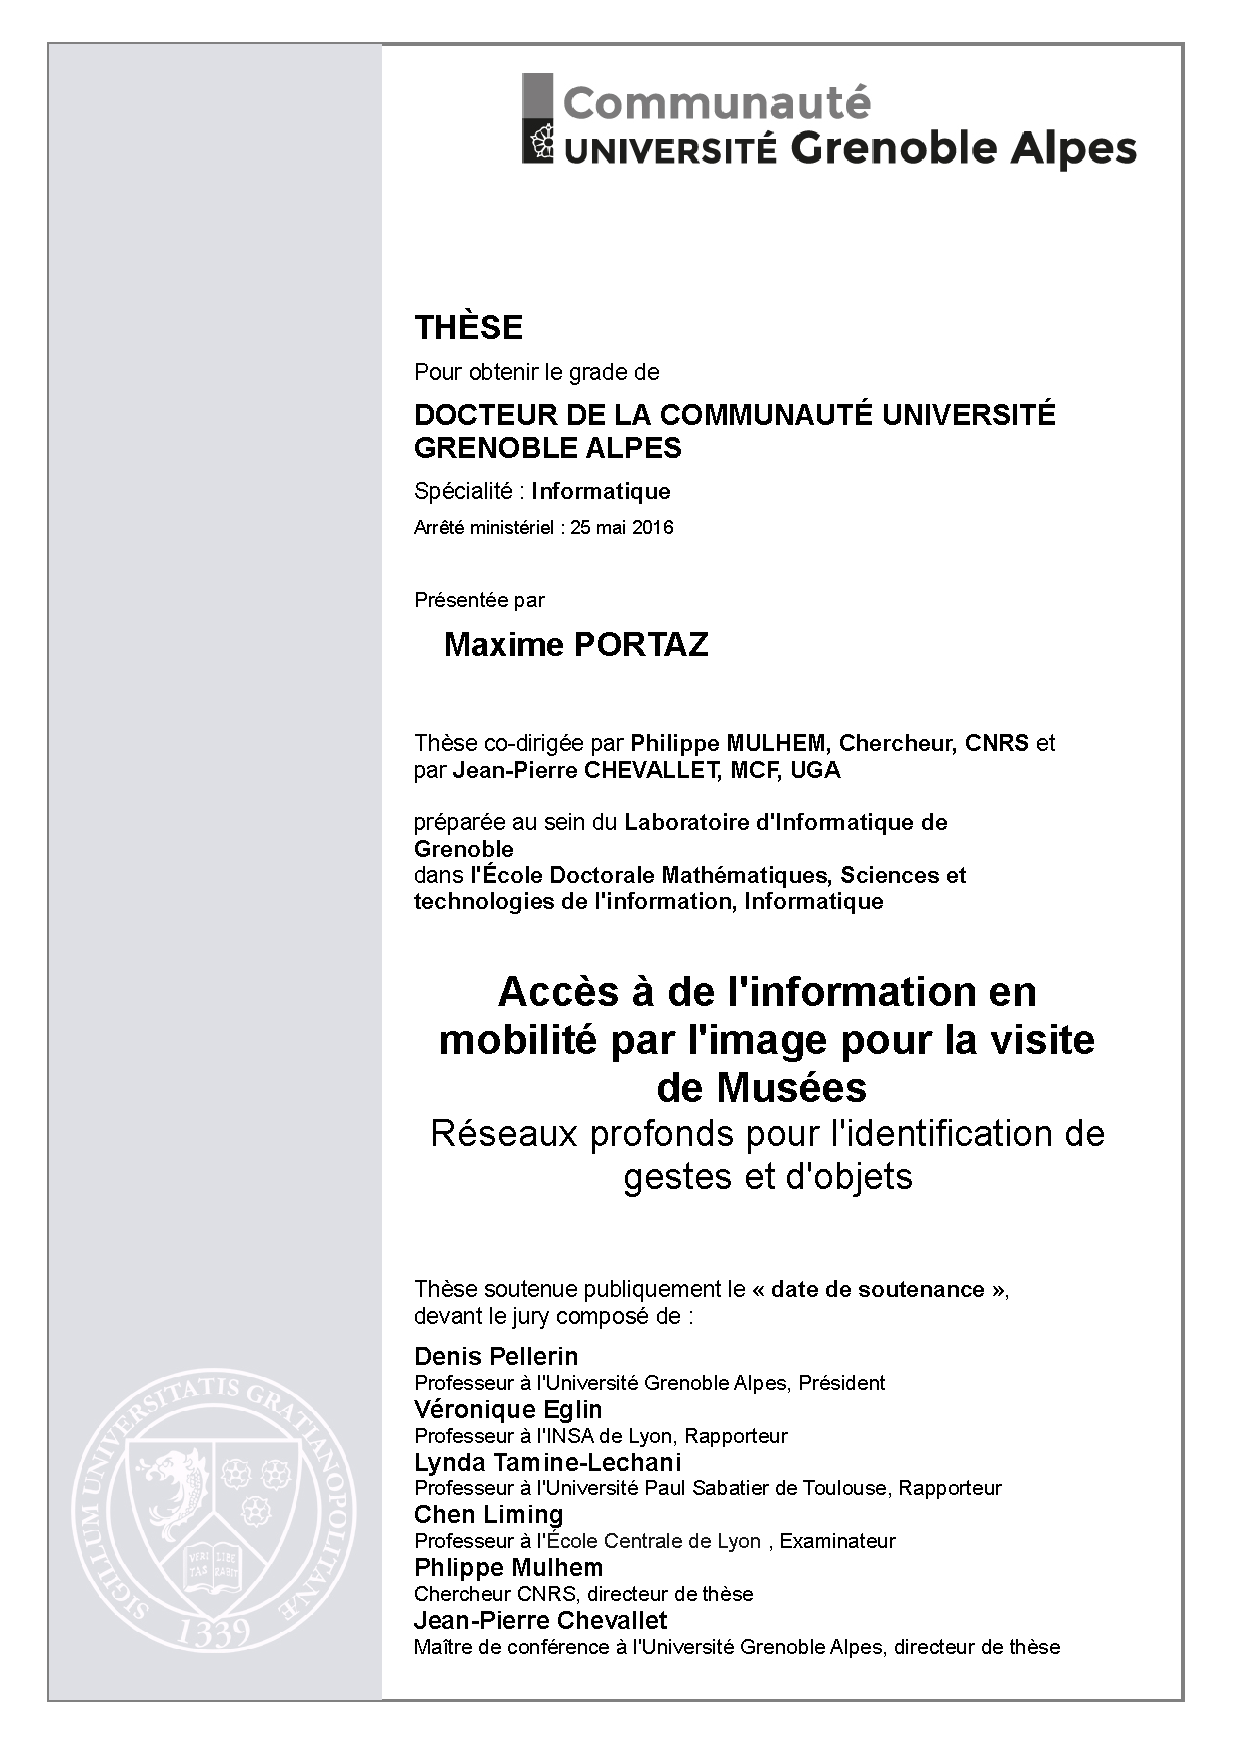
\includepdf[pages={1}]{couverture_thesePerso.pdf}
\newpage
~
\newpage
% the front matter
% some details about the thesis
\title{Titre}
\englishtitle{Title}
\author{Maxime Portaz}
\advisor{Philippe Mulhem, Jean-Pierre Chevallet}

% about the degree
\degree{Docteur de la communauté université Grenoble Alpes}
\field{Informatique}
\degreeyear{2018}
\degreemonth{Septembre}

% about the university
\department{Laboratoire d'Informatique de Grenoble}
\university{Université Grenoble Alpes}
\universitycity{Grenoble}
\universitystate{France}
\maketitle
\copyrightpage

\pageresume

\abstractpage

\dedicationpage

\acknowledgments

\tableofcontents
%\authorlist

\listoffigures

\justify
% include each chapter...

\pagenumbering{arabic}

\chapter{Introduction}

%
% Vérifier intro problématique corpus
%
%
%%%%%%%%%%%%%%%%%%%%%%%%%%%%%%%%%%%%%%%%%%%%%%%%%%%%%%%%%%%%%%%%%%%%%%%%%%%%%%%%%%%%%%%%%%%%%%%%%%%%%%%%%%%%%%
% Présentation Contexte
% Présenter le projet, le contexte. GUIMUTEIC, caméra, visite, action utilisateur.
% Aide à l'utilisateur : réagir à l'intention de l'utilisateur, approt d'information sur ce qui est regardé
\section{Le Contexte de cette thèse}
%(Ajouter : on utilise indifféremment utilisateur ou visiteur).

Les sites touristiques, et notamment les musées, ont su assimiler les évolutions technologiques et proposer de nouvelles méthodes d'interaction pour enrichir les visites et les rendre davantage personnalisées.
La visite d'un site touristique peut être accompagnée d'un guide, qu'il s'agisse d'un humain (un guide culturel), ou d'une aide électronique.
Ces nouveaux outils, pouvant être mobiles ou fixes comme des bornes multimédia, ne remplacent pas un guide humain, mais permettent de fournir des informations visuelles (visio-guide) ou des informations audio (audio-guide), tout en réduisant la fatigue liée à la visite de musée sans aide~\cite{bitgood2009museum}.
Grâce aux avancées techniques, telles que la réduction de la taille des capteurs ou la puissance des processeurs mobiles, les possibilités des outils mobiles s'enrichissent. Et permettent même l'arrivée de solutions à base de réseaux de neurones profonds~\cite{howard2017mobilenets}.

Les guides électroniques permettent d'influencer les visites de musées, le visiteur restant plus longtemps et analysant plus en détail les œuvres~\cite{lanir2013influence}.
Malgré le fait qu'ils puissent, dans certains cas, gêner l'interaction sociale des visiteurs en groupes~\cite{lanir2013influence, grinter2002revisiting}, il est au contraire possible, grâce à un bon design, de promouvoir les échanges~\cite{gammon2008designing}.
En examinant les impacts des nouveaux usages des visiteurs~\cite{andreacola2014musee}, nous pouvons imaginer de nouvelles pratiques, avec notamment des visites plus personnalisées.
Que ce soit à travers la réalité augmentée ou l'identification automatique du contexte dans lequel se trouve l'utilisateur, ces systèmes reposent sur des procédés capables de reconnaître l'environnement qui entoure l'utilisateur.
Nous utiliserons dans la suite indifféremment utilisateur ou visiteur, car nous nous situons dans l'environnement de la visite de musées.

Cette thèse s'inscrit, avec un financement européen, dans le cadre d'un projet du Fonds Unique Interministériel (FUI) : Guide Multimédia de Tête, Informatif et Connecté (GUIMUTEIC).
Ce projet a pour but de proposer une nouvelle génération de guides pour les visites de musée.
Le dispositif GUIMUTEIC est équipé de différents capteurs, notamment une caméra.
Il est prévu pour être porté par chaque utilisateur et est destiné à enrichir la visite, en la personnalisant et en facilitant l'interaction.
Pour cela, le système GUIMUTEIC doit être capable d'identifier les points d'intérêts regardés par l'utilisateur, de le renseigner lorsque celui-ci le désire, et de réagir en fonction de ses actions.
Ce travail de thèse explore donc les besoins d'identification d'œuvres, d'actions et de l'environnement de l'utilisateur.



%\begin{figure}%
%\centering
%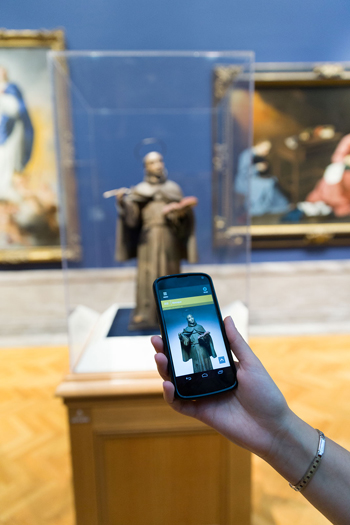
\includegraphics[width=\textwidth/3]{figures/ArtLens.jpg}%
%\caption{Exemple de visite avec une guide sur smartphone}%
%\label{fig:exemplevisite}%
%\end{figure}

\begin{figure}%
\centering
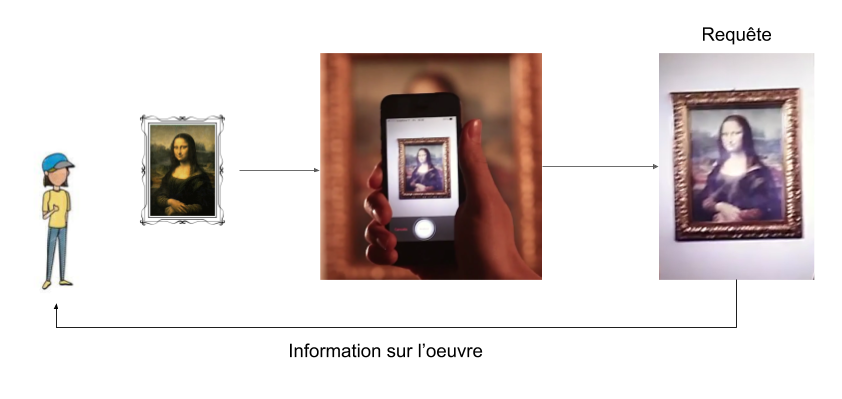
\includegraphics[width=\textwidth]{figures/Requete.png}%
\caption{Exemple d'une aide à la visite avec un smartphone. L'utilisateur peut prendre en photo une œuvre pour avoir des informations sur celle-ci.}
\label{fig:exemplevisitesmartphone}%
\end{figure}

%%%%%%%%%%%%%%%%%%%%%%%%%%%%%%%%%%%%%%%%%%%%%%%%%%%%%%%%%%%%%%%%%%%%%%%%%%%%%%%%%%%%%%%%%%%%%%%%%%%%%%%%%%%%%%
% PROBLEMATIQUE
% Reco d'oeuvre
% Reco d'action
% Reco de contexte
% Travail sur image et vidéo
\section{Problématiques de la recherche d'information muséale}
\label{sec:introcontraintes}
Les problématiques soulevées portent sur l'aide pouvant être apportée à l'utilisateur et les moyens d'interactions avec le dispositif mobile.
Équipé du dispositif GUIMUTEIC, intégrant une caméra embarquée, le but est de fournir à l'utilisateur une information sur son environnement, notamment les œuvres se trouvant face à lui.
Pour cela, il est nécessaire d'utiliser des méthodes d'identification d'instances précises.
Nous référons ici par ``{\it Instance}'', l'instance d'un objet, par exemple la Joconde, par opposition à une classe d'objet, dans ce cas un tableau.
Nous avons également besoin de déterminer si, et à quel moment, l'utilisateur désire avoir accès à de l'information à propos d’une œuvre.
En prenant comme exemple le musée de Bibracte\footnote{\url{http://www.bibracte.fr/}}, où certaines actions se déclenchent quand le visiteur entre dans une pièce, on comprend l'intérêt de réagir en fonction des actions de l'utilisateur.
La localisation de l’utilisateur seule n’est pas toujours suffisante lorsque l’on s’intéresse à identifier son environnement, en ne prenant pas en compte l’orientation ou ce à quoi l’utilisateur s’intéresse~\cite{schmidt1999there}.
C’est pourquoi nous allons nous intéresser à détecter des points d’intérêts que le visiteur regarde, en plus d’identifier ses actions grâce à de la détection de geste par le dispositif GUIMUTEIC.


%%%%%%%%%%%%%%%%%%%%%%%%%%%%%%%%%%%%%%%%%%%%%%%%%%%%%%%%%%%%%%%%%%%%%%%%%%%%%%%%%%%%%%%%%%%%%%%%%%%%%%%%%%%%%
% CONTRAINTES du projet
% Puissance limité
% Limitation sur les corpus
%\section{Contraintes du projet GUIMUTEIC}
%\label{sec:introcontraintes}
En dehors des problématiques scientifiques énoncées ci-dessus, ce travail s'inscrit dans le cadre d'un projet ``industriel''.
Ceci définit un certain nombre de contraintes qui vont influencer les choix effectués par la suite.
Tout d'abord, le système GUIMUTEIC est à destination de sites touristiques pouvant être de natures différentes, que ce soit en plein air ou en intérieur.
De même, le type des œuvres présentes dans un musée est très variable, de pierres taillées dans un musée d'archéologie, à des peintures ou des œuvres abstraites dans un musée d'art moderne, en passant par des voitures ou des pièces de monnaie.
L'objectif est de fournir une solution générale, pouvant s'adapter à chacun.

Une autre contrainte, directement liée au caractère industriel du projet, est l'effort de mise en place dans chacun des musées, qui doit être minimisé.
L'acquisition des données, la quantité de données recueillies ou l'annotation de ces données, sont des opérations coûteuses qui doivent être limitées.
L'objectif étant de proposer une solution applicable aisément à chaque musée, le travail demandé pour la mise en place doit être aussi réduit que possible.
L'étude de ces contraintes et de leurs impacts sur les choix pouvant être fait sera présentée dans le chapitre~\ref{chap:etude} intitulé~``\nameref{chap:etude}''.




%%%%%%%%%%%%%%%%%%%%%%%%%%%%%%%%%%%%%%%%%%%%%%%%%%%%%%%%%%%%%%%%%%%%%%%%%%%%%%%%%%%%%%%%%%%%%%%%%%%%%%%%%%%%%
% OBJECTIFS et CONTRIBUTION
\section{Contributions}

Les objectifs de cette thèse sont multiples : nous nous intéresserons à la reconnaissance d'instances et à l'exploration de différentes méthodes d'interaction avec l'utilisateur, tout en respectant les contraintes imposées par le projet GUIMUTEIC.


Ce travail de thèse apporte les contributions suivantes :
\begin{description}
	\item[Étude de l'accès à l'information pendant une visite touristique] La première contribution de ce travail de thèse concerne l'étude des visites de musées et les besoins en terme d'accès à l'information au cours des visites touristiques. Nous proposons un système mobile d'interaction entre l'utilisateur et le dispositif, qui permet de répondre aux attentes des musées et du projet GUIMUTEIC.
	\item[Reconnaissance d'instances] Nous proposons également une approche pour l'identification d'instances, dans le but de reconnaître les scènes vues par l'utilisateur. Pour cela, nous présentons un nouveau système de recherche d'image à base de réseaux de neurones siamois, pour l'apprentissage de similarité entre les images,.
	\item[Apprentissage des régions d'intérêt] Dans le but d'améliorer la reconnaissance d'instances, nous exposons une nouvelle méthode d'apprentissage automatique des régions d'intérêt dans les images. Cette méthode se base sur un apprentissage non supervisé des zones de l'image, et ne nécessite pas d'annotation de régions sur les images. Nous étudions l'apport de cette détection sur l'apprentissage de similarité, et comment apprendre les deux conjointement.
	\item[Détection de geste] Pour proposer une interaction avec l'utilisateur, nous cherchons à détecter ses gestes et actions grâce au dispositif GUIMUTEIC, c'est-à-dire avec une vue égocentrique (à la première personne). Nous développons pour cela un nouveau système de reconnaissance de gestes dans les vidéos à base de réseaux de neurones à convolutions, sans récursion.
	\item[Création de corpus d'évaluations] Pour vérifier la faisabilité du système développé dans des conditions réelles, nous avons recueilli plusieurs corpus dans les musées partenaires du projet. Tous les algorithmes développés dans cette thèse sont évalués sur ces corpus. La collecte et l'organisation de ces corpus sont présentées en annexe~\ref{chap:corpus} intitulée ``\nameref{chap:corpus}’’.
\end{description}


\subsection{Publications}

Le travail développé dans cette thèse à fait l'objet des publications suivantes :

\begin{itemize}
	\item \bibentry{portaz2018object}
	\item \bibentry{portaz2017fully}
	\item \bibentry{portaz2017construction}
	\item \bibentry{portaz2016etude}
	\item \bibentry{portaz2016mrim}
\end{itemize}

Le code développé ainsi que les collections créées dans cette thèse sont librement disponibles.
Pour le code utilisé pour les expérimentations, et également les schémas et les tableaux présentés, sont disponibles sur GitHub à l'adresse \url{https://github.com/maxgreat}.
Les collections d'images et de vidéos sont disponibles en accès libre dans le cadre de la recherche à l'adresse~\url{http://lig-mrim.imag.fr}.



%%%%%%%%%%%%%%%%%%%%%%%%%%%%%%%%%%%%%%%%%%%%%%%%%%%%%%%%%%%%%%%%%%%%%%%%%%%%%%%%%%%%%%%%%%%%%%%%%%%%%%%%%%%%%
% ORGANISATION de la thèse
\section{Plan du manuscrit}

Afin de décrire le travail mené dans le cadre de cette thèse nous suivons le plan suivant :


\begin{description}
	\item[Chapitre~\ref{chap:etude}:~\nameref{chap:etude}] Nous réalisons tout d'abord une étude approfondie du problème d'accès à l'information dans le cadre de visites touristiques.
Nous analysons plus en détail les contraintes spécifiques des musées.
Nous nous intéressons particulièrement aux différents moyens d'accès à l'information possibles dans ce contexte, et notamment aux types d'interactions avec l'utilisateur envisageables et désirables pour les visiteurs.

	\item[Chapitre~\ref{chap:stateoftheart}:~\nameref{chap:stateoftheart}] Nous introduisons différentes méthodes de recherche d'informations multimédia et d'analyse d'images existantes dans la littérature.
Nous présenterons l'état de l'art de la recherche d'images, particulièrement les techniques de réseaux de neurones profonds (Deep Learning).
Un état de l'art de la détection d'évènements dans les vidéos est aussi présenté.

	\item[\textbf{Chapitre~\ref{chap:similarite}:~\nameref{chap:similarite}}] Dans ce chapitre, nous présentons l'analyse et la modélisation du problème d'identification d'œuvres dans les images et vidéos.
Nous explorons différentes méthodes basées sur ce qui a été présenté dans le chapitre~\ref{chap:stateoftheart}, et nous les adaptons à nos problématiques. Nous évaluons ces méthodes sur les corpus d'images construits. 

\item[\textbf{Chapitre~\ref{chap:regions}:~\nameref{chap:regions}}] Nous fournissons une nouvelle méthode pour la détection de régions d'intérêt dans les images. Grâce à un apprentissage de la localisation des objets dans les images, sans annotation des régions sur le corpus d'apprentissage, nous obtenons des résultats supérieur à l'état de l'art sur nos collections. 

	\item[\textbf{Chapitre~\ref{chap:gestes}:~\nameref{chap:gestes}}] Ce chapitre est consacré à l'étude de la détection des actions de l'utilisateur dans les vidéos.
Suite à l'étude réalisée dans le chapitre~\ref{chap:etude}, nous nous intéressons aux gestes nécessaires à l'interaction et aux méthodes de détection possibles. Nous étudions la détection des gestes avec une vue à la première personne. Nous utilisons des réseaux de neurones non récursifs, avec pour objectif d'avoir un réseau de neurones compact et rapide, utilisable sur mobile. Nous évaluons notre approches grâce à un corpus de vidéos créé spécialement.

	\item[\textbf{Chapitre~\ref{chap:conclusion}:~\nameref{chap:conclusion}}] Finalement, le dernier chapitre présente la démarche générale. Nous concluons sur les contributions de ce travail de thèse, notamment sur les méthodes d'identifications d'instance et de détection de gestes à l'aide de réseaux de neurones profonds et sur la création du système GUIMUTEIC, ainsi que sur la suite des recherches possibles sur les problématiques présentées.

\end{description}





%\chapter{Etude des besoins et contraintes dans les visites touristiques}
\chapter{Les enjeux de l'interaction dans les visites touristiques}
\label{chap:etude}

L'objectif de ce travail de thèse est de répondre aux problématiques d'accès à l'information durant les visites touristiques. 
Ce chapitre va étudier en détail les besoins et les attentes des musées et des visiteurs dans le cadre des nouveaux types d'interaction existants à l'heure actuelle.
En s'intéressant notamment à une interaction à base de gestes, développée grâce à une étude utilisateur réalisée avec des séances participatives.

Les raisons de créer de nouveaux moyens d'interaction dans les musées sont multiples (section~\ref{sec:nouveauxmoyendinteraction}), ce qui implique de réfléchir à de nouvelles méthodes d'accès à l'information. 
Le projet GUIMUTEIC (section~\ref{sec:GUIMUTEIC}) doit répondre à ces besoins, tout en respectant ses contraintes de déploiement. 


\section{Les nouveaux moyens d'interaction et d'accès à l'information muséale}
\label{sec:nouveauxmoyendinteraction}

Les professionels des musées, ainsi que les visiteurs, ont vu leur compréhension de ce qu'est un musée changer, avec l'introduction de nouvelles technologies au sein des musées~\cite{knell2010shape}.
Le problème des nouvelles interactions n'est pas que technologique, il nécessite une étude interdisciplinaire des intéractions sociales et technologiques dans les musées, comme le souligne le ``museum informatics'' défini par Marty~\cite{marty2008museum}.


L'essor des sciences de l'information et des technologies a créé de nouveaux moyens d'accès et de traitement de l'information dans les musées, et une nouvelle manière de penser les musées est apparue~\cite{marty2011my}. 
Les musées ont traditionnellement servi de recueil d'objets, dans le but de les préserver, de les étudier ou d'éduquer. 
Cependant, ils ne sont pas là uniquement pour stocker des objets.
Même si la partie fondamentale d'un musée reste sa collection d'œuvres et d'objets, la grande quantité d'information disponible à propos de chacun de ces objets est tout aussi importante~\cite{greenhill1992museums}.
Les visiteurs s'attendent aujourd'hui à avoir un accès instantané à toutes les connaissances du musée à propos de chaque œuvre. Pour rendre cela possible, il a été établi depuis longtemps que les musées se devaient de proposer de nouveaux moyens de gérer l'information~\cite{keene1996becoming}.
Chaque visiteur est unique, avec des attentes différentes, et ce qu’il retiendra d'une visite va dépendre des objets vus, du personnel du musée, du contexte socioculturel et de certains aspects propres à la personne~\cite{falk2016identity}.
Il est important d'avoir une personnalisation de la visite pour que chacun puisse avoir la meilleure expérience, adaptée à ces besoin.
Par exemple, le projet PIL~\cite{kuflik2011visitor} propose une réflexion sur comment adapter le musée au visiteur, grâce aux outils technologiques, tout en faisant en sorte que celui-ci soit concentré sur les expositions et non pas sur les appareils de visites.
Il faut notamment faire attention à ce que les outils technologiques ne bloquent pas la communication avec les autres visiteurs. Ils ne doivent pas être invasifs pendant la visite, pour que l'utilisateur puisse se concentrer sur les œuvres.
 
Il est commun aujourd'hui d'avoir un audio-guide (ou un visio-guide) dans les musées afin d'avoir une audio(visio)-description d'une œuvre d'art, son impact sur la visite n'est donc pas à négliger.
Les guides permettent de garder les utilisateurs plus longtemps à l'intérieur du musée, en passant plus de temps à étudier les oeuvres, tout en s'intéressant à davantage d'oeuvres~\cite{lanir2013influence}. 
Ils permettent également d'améliorer l'interaction avec l'utilisateur~\cite{evans1999portable} ainsi que de renforcer le côté éducatif de la visite~\cite{woodruff2002eavesdropping}.
Cependant, les guides électroniques ont tendance à fermer les personnes à l'interaction sociale~\cite{angliss2006talking}. Dans le cas de visites en groupes, les appareils mobiles forcent l'utilisateur à regarder l'écran et à ne pas faire attention aux personnes avec lesquelles il est venu~\cite{grinter2002revisiting, petrelli2005user}.
Il devient également fréquent d'avoir accès à l'information directement sur son smartphone.
Ceux-ci ont le problème de couper le visiteur de ce qui l'entoure, car il va regarder son téléphone plutôt que ce qui l'entoure. Comme il est devenu clair qu'il était difficile de détourner une personne de son smartphone, celui-ci peut être utilisé par le musée pour guider le visiteur ou fournir un plus à la visite~\cite{gammon2008designing, pierroux2011bridging, weilenmann2013instagram}.
Pour ne pas détourner l'attention des utilisateurs envers les œuvres, ni couper le visiteur de son groupe, le projet GUIMUTEIC n'utilise pas d'écran, mais uniquement un casque audio ouvert.

Plusieurs approches modernes proposent de nouvelles interfaces technologiques, pour l'interaction avec les œuvres culturelles.
Par exemple, le ``SmartMuseum''~\cite{kuusik2009smartmuseum} propose à l'aide de capteurs RFID (Radio Frequency Identification) de donner des informations au visiteur. 
Ce dernier peut construire sa propre visite sur le site web en amont de sa venue, et reconnaître sur site les œuvres sélectionnées.
L'utilisation d'étiquettes RFID limite, ou complexifie, la modification de l'organisation du musée. Le maintien et l'organisation de la base d'étiquette devient une contrainte et demande un certain engagement de la part du musée. 
Ce système requiert l'utilisation d'un appareil mobile et de plus requiert un certain degré d'apprentissage dans son utilisation.

Une solution pour aider le visiteur est d'utiliser un appareil mobile qui sert de guide audio-visuel, comme le propose le ``Museum Wearable''~\cite{sparacino2002museum}. L'appareil utilise la connaissance de l'environnement de l'utilisateur pour lui fournir l'information sur ce qui l'intéresse à un instant donné. Ce prototype utilise uniquement la position géographique de l'utilisateur pour déterminer son environnement, or la position seule n'est pas nécessairement suffisante pour déterminer le contexte autour de l'utilisateur~\cite{schmidt1999there}.
Une caméra par exemple permet d'obtenir plus d'information, et si celle-ci est positionnée de manière à voir ce que l'utilisateur perçoit, avec une vue à la première personne. On est alors capable d'avoir une information précise sur l'environnement direct.

Pour déterminer ce qui intéresse le visiteur, des méthodes d'interaction à base de gestes ont été développées. 
L'approche à base de systèmes portatifs avec vision à la première personne~\cite{baraldi2015gesture} permet de voir ce que l'utilisateur perçoit, de réagir à ces gestes et d'avoir des informations précises sur son environnement. 
Comme montré sur la figure~\ref{fig:exempleGestea}, un utilisateur, équipé de lunettes avec caméra embarquée, peut interagir avec celles-ci grâce à une série de gestes prédéfinis (figure~\ref{fig:exempleGesteb}). 
Ici les gestes sélectionnés sont Approuver (``OK''), Désapprouver (``Dislike''), Défiler (``Slide''), Valider (``Like''), Pointer et Prendre une photo (``Take a picture'').
Ces gestes n'ont cependant pas été développés avec une étude utilisateur.
Ce type d'approches permet de dépasser les limitations des appareil mobiles qui requièrent une manipulation et qui détourne l'attention de l'utilisateur des œuvres. 
Ceci permet également de proposer de nouvelles expériences d'interaction, et d'encourager le visiteur à interagir avec les œuvres, comme ils le feraient devant un guide humain. 
Si de tels gestes sont utilisés, il faut cependant étudier l'utilité des gestes reconnus, et lesquels sont les plus à même de correspondre aux attentes des utilisateurs. 
Il faut ensuite déterminer à quelle moment de la visite réaliser la reconnaissance d'environnement de l'utilisateur, et notamment reconnaître les œuvres en face de lui, pour lui fournir une réponse à son interaction.


\begin{figure}[htbp]
\begin{subfigure}{0.49\textwidth}
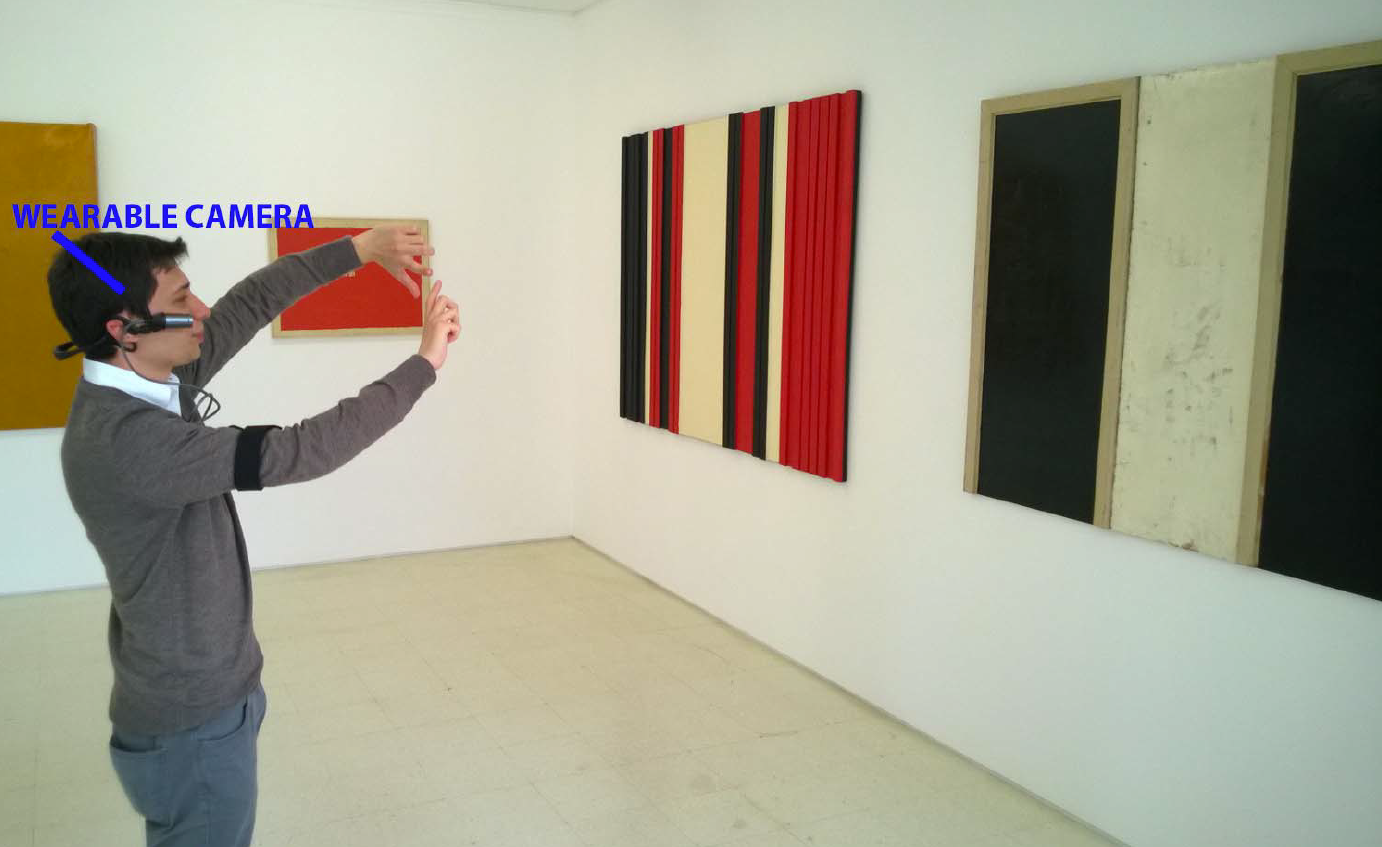
\includegraphics[width=\linewidth]{figures/wearable.PNG}
\caption{Geste en face d'une oeuvre} \label{fig:exempleGestea}
\end{subfigure}
\hspace*{\fill} % separation between the subfigures
\begin{subfigure}{0.49\textwidth}
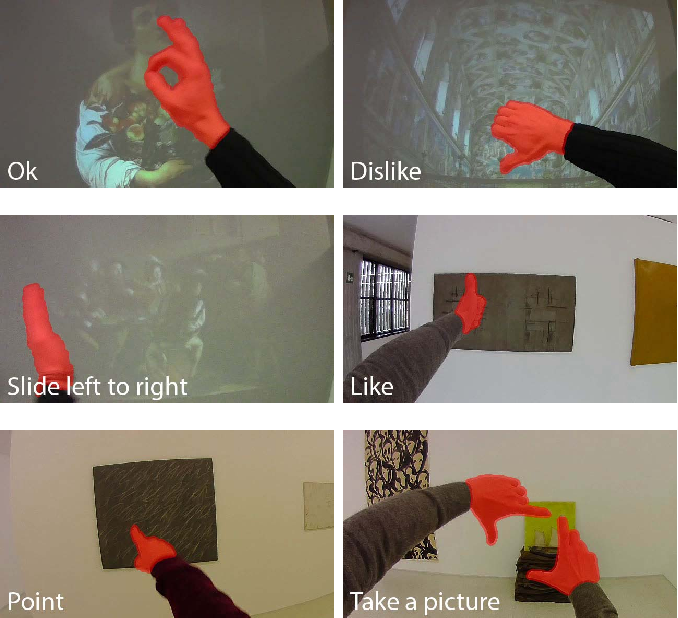
\includegraphics[width=\linewidth]{figures/gesteBaradli.png}
\caption{Gestes selectionnés} \label{fig:exempleGesteb}
\end{subfigure}
\caption{Exemple d'un système basé sur l'interaction à base de geste dans un musée~\cite{baraldi2015gesture}} \label{fig:exempleGeste}
\end{figure}




%%%%%%%%%%%%%%%%%%%%%%%%%%%%%%%%%%%%%%%%%%%%%%%%%%%%%%%%%%%
%
%   Le système GUIMUTEIC
%
%%%%%%%%%%%%%%%%%%%%%%%%%%%%%%%%%%%%%%%%%%%%%%%%%%%%%%%%%%%
\section{Le système GUIMUTEIC}
\label{sec:GUIMUTEIC}

Le système GUIMUTEIC est un système mobile, doté d'une caméra, aidant et améliorant la visite de musées. 
Pour cela, il doit être capable d'identifier les actions de l'utilisateur, et de réagir à ses besoins. 
Il doit également pouvoir reconnaître l'environnement de ce dernier, pour le guider et lui apporter les informations correspondantes à ce qu'il regarde. 

Avec une série d'études participatives, nous avons identifié les types d'interaction adaptées au projet (paragraphe~\ref{sec:gestesGUIMUTEIC}). Ainsi, tout en respectant les contraintes liées au projet (paragraphe~\ref{sec:contraintesGUIMUTEIC}), nous avons pu mettre au point un système d'aide au visiteur qui répond à ses besoins (paragraphe~\ref{sec:systemeGUIMUTEIC}). 



%%%%%%%%%%%%%%%%%%%%%%%%%%%%%%%%%%%%%%%%%%%%%%%%%%%%%%%%%%%
%
%   Les Gestes GUIMUTEIC
%
%%%%%%%%%%%%%%%%%%%%%%%%%%%%%%%%%%%%%%%%%%%%%%%%%%%%%%%%%%%
\subsection{Une interaction à base de gestes}
\label{sec:gestesGUIMUTEIC}

Des séances participatives de conception d'un appareil d'aide à la visite de musée ont été organisées. 
Regroupant des participants de différents âges et antécédents, elles ont permis, grâce à des exercices ludiques, de définir les usages futurs du dispositif, et de mettre en avant ce que les utilisateurs finaux attendent du produit. 
Ces séances ont fait ressortir plusieurs méthodes d'interaction susceptibles d'être intéressantes pour les visiteurs.
Les détails de cette étude sont reportés dans l'annexe~\ref{sec:etudeGestes}~``\nameref{sec:etudeGestes}’’.

\`A l'issue de ces séances, l'interaction privilégiée est celle à base de gestes. Cinq gestes ont été identifiés comme utiles à l'interaction, et sont présentés dans la figure~\ref{fig:photoGestes}. Il s'agit de \textbf{pointer}, signaler \textbf{``OK''}, \textbf{valider (ou ``liker'')}, \textbf{arrêter} et \textbf{stop} (ou pause).  

\begin{figure}[!htb]
	\begin{minipage}[c]{.32\linewidth}
		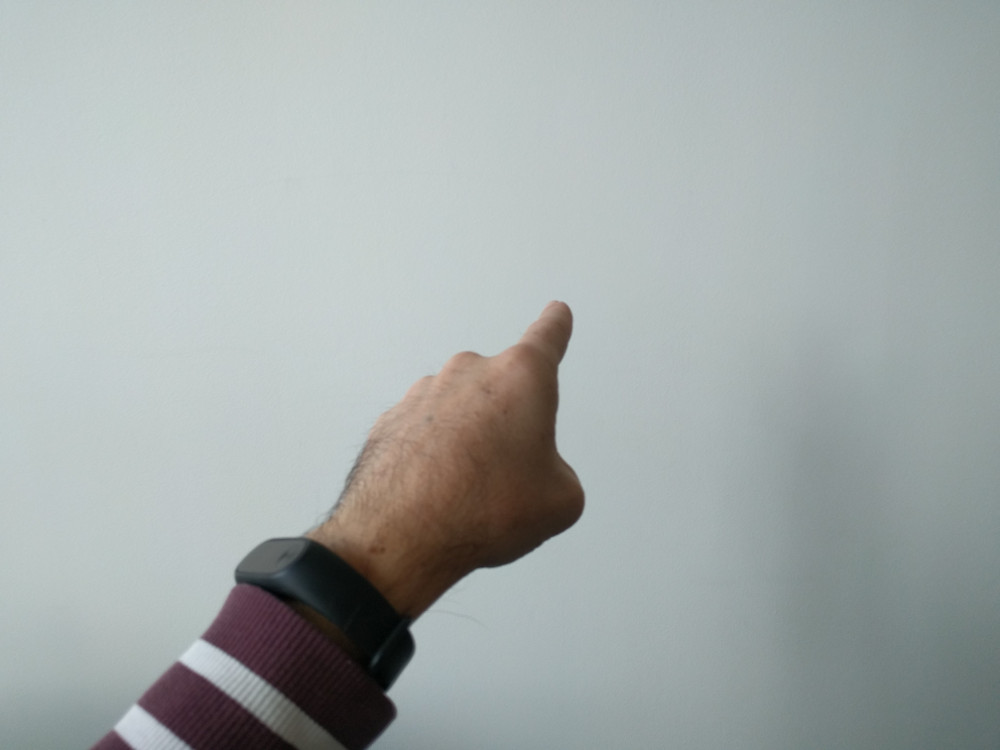
\includegraphics[width=\columnwidth]{figures/1.jpg}%
		\caption*{Pointer}%
	\end{minipage} \hfill
	\begin{minipage}[c]{.32\linewidth}
		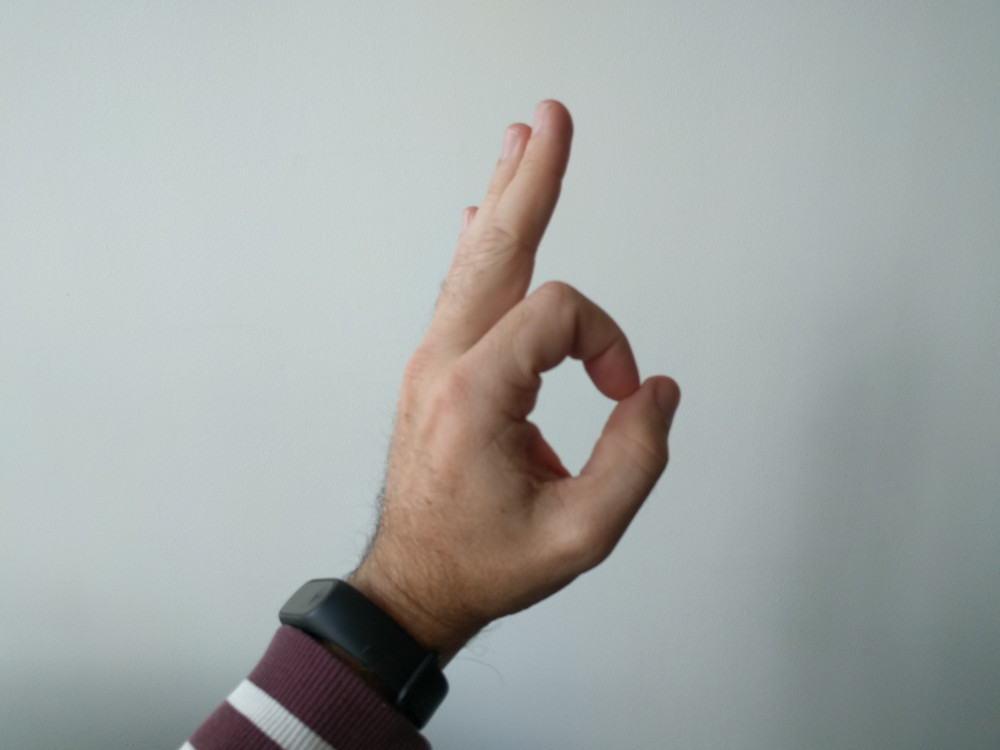
\includegraphics[width=\columnwidth]{figures/2.jpg}%
		\caption*{OK}%
	\end{minipage} \hfill
	\begin{minipage}[c]{.32\linewidth}
		
\includegraphics[width=\columnwidth]{figures/3.jpg}%
		\caption*{Valider}%
	\end{minipage}
	\centering
	\begin{minipage}[c]{.32\linewidth}
		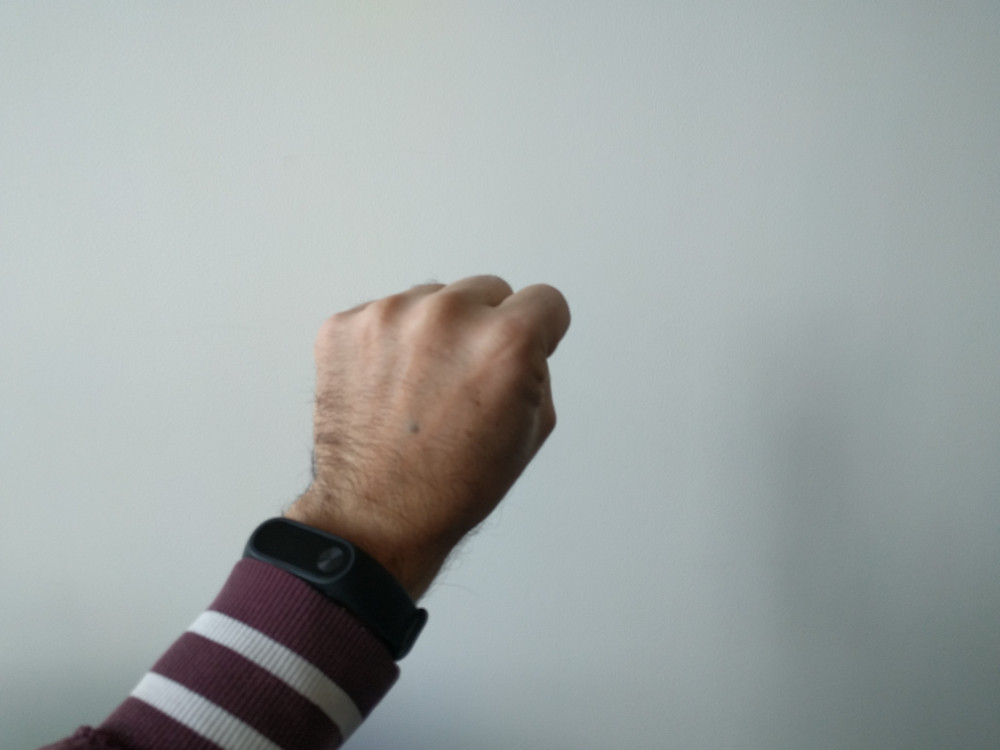
\includegraphics[width=\columnwidth]{figures/4.jpg}%
		\caption*{Arrêter}%
	\end{minipage}
	\begin{minipage}[c]{.32\linewidth}
		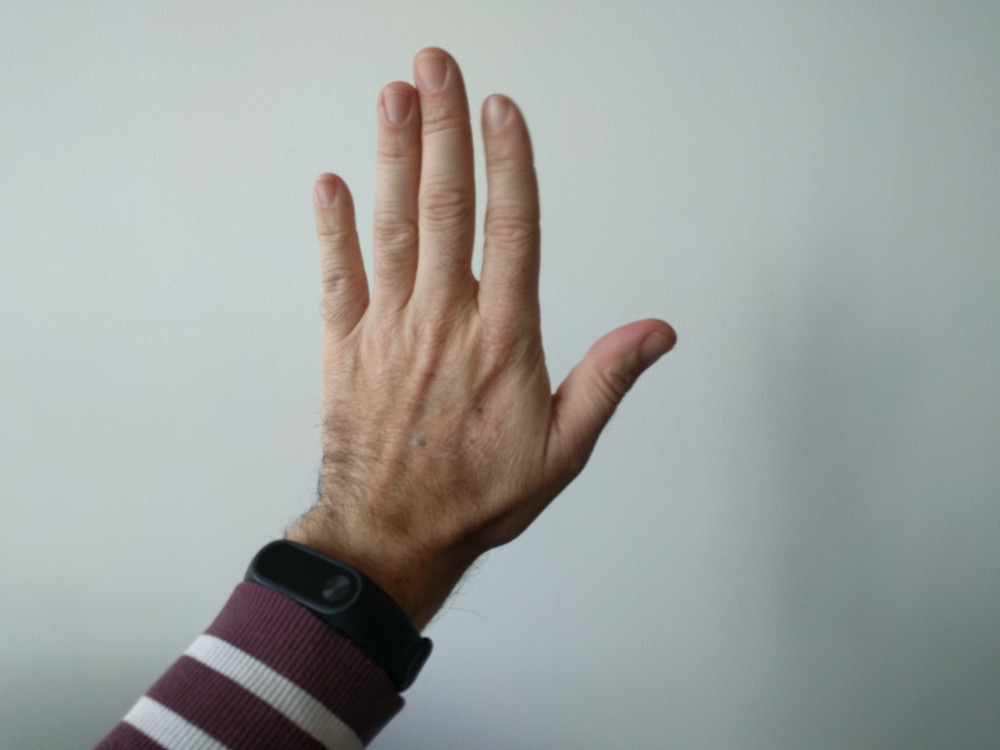
\includegraphics[width=\columnwidth]{figures/5.jpg}%
		\caption*{Stop}%
	\end{minipage}
	\caption{Les 5 gestes mis en avant par les séances de conceptions participative.}
	\label{fig:photoGestes}
\end{figure}

Pour créer un système de reconnaissance de ces gestes, un ensemble de vidéos de gestes correspondant aux attentes du projet ont été réalisés. 
Ce corpus est composé de vidéos en vue à la première personne, prise dans différentes conditions, avec des environnements différents et notamment sur fond vert. 
La description complète du corpus est fournie en annexe~\ref{sec:etudeGestes}. 
Les méthodes proposées dans le chapitre~\ref{chap:gestes} seront testées sur ce corpus.





%%%%%%%%%%%%%%%%%%%%%%%%%%%%%%%%%%%%%%%%%%%%%%%%%%%%%%%%%%%
%
%   Les Contraintes GUIMUTEIC
%
%%%%%%%%%%%%%%%%%%%%%%%%%%%%%%%%%%%%%%%%%%%%%%%%%%%%%%%%%%%
\subsection{Les contraintes des musées et du projet GUIMUTEIC}
\label{sec:contraintesGUIMUTEIC}

Le projet GUIMUTEIC est le fruit d'une collaboration industrielle, et doit donc répondre à un certain nombre de contraintes qui en découlent.
Le premier type de contraintes est lié à la distributivité du produit. Le système doit être capable d'être applicable à n'importe quel type de musée. 
Dans le cadre du projet, deux types de musées sont étudiés: un musée d'archéologie, le musée Gallo-Romain de Lyon Fourvière, et le musée d'art de Grenoble. 
Les types d'objets présents dans ces musées étant variés, leur étude nous permet de produire un système généralisable. 

Un autre facteur important de la faisabilité de ce type de projet, est le coût, en infrastructure et en heures, de l'installation du système dans un musée. 
Compte tenu de l'aspect portatif de dispositif GUIMUTEIC, il est important qu'aucune connexion permanente à un serveur ne soit nécessaire. 
En effet, la connection à un serveur distant sous-entend, en plus de la présence et de la maintenance de serveurs, une connectivité dans l'ensemble du musée. 

Pour être utilisable par le plus de personnes possible, un guide doit pouvoir être utilisé sans apprentissage de la part de la personne qui l'utilise, pour ne pas décourager celle-ci, et permettre à n'importe qui de l'utiliser de manière simple, sans formation. 
De plus, le système doit fonctionner sans apprentissage de la part du système pour chaque utilisateur. 
Il doit être capable de s'adapter à toutes les morphologies, de taille notamment, et de couleur de peau.

De la même manière, pour la mise en place de la reconnaissance d'environnements et d'œuvre autour de l'utilisateur, une base de données des lieux, œuvres et autres points d'intérêt du musée, doit d'être constituée. 
Ceci pouvant être un frein considérable à l'installation d'un nouveau système, du fait du coût en heures de prise de vues et en maintenance, nous avons de forte contraintes sur la création de cette base. 
Nous nous limitons à quelques photos par œuvre et point d'intérêt du musée. 
La capture de vidéos de visite est un processus très coûteux: en plus de l'enregistrement, qui doit faire intervenir un certain nombre de personnes pour avoir une diversité suffisante, il faut prendre en compte le coût de l'annotation de chacune de ces vidéos.
Identifier quel objet est visible à chaque instant, si possible même annoter la position de l'objet dans l'image, est long et nécessite un certain investissement, qui ne correspond pas au projet dans lequel nous nous situons.
Les propositions dans la suite de cette thèse doivent donc répondre à ces contraintes :

\begin{itemize}
	\item Quelques images par œuvre : la reconnaissance d'instance dans les images doit pouvoir se faire avec seulement quelques exemples de ladite instance comme référence.
	\item Portabilité de l'appareil : la quantité de calcul et l’utilisation de la mémoire pour le reconnaissance d'actions et d'instances doivent être aussi limités que possible, en ayant comme objectif de tout réaliser sur un processeur mobile.
	\item Pas de vidéos de visite : la réalisation de vidéos de visite complètes, annotées, demande trop d'investissement. Nous partons donc du principe que nous ne disposons pas de ce type de vidéos.
\end{itemize}





\subsection{Le système d'interaction GUIMUTEIC}
\label{sec:systemeGUIMUTEIC}

Notre approche pour la création d'une aide à la visite muséale est présentée dans le schéma~\ref{fig:actioncontexte}.
L'utilisateur, libéré de tout appareil dans ses mains, peut interagir avec le système GUIMUTEIC à travers des gestes prédéfinis.
On voit sur la figure le visiteur sur la gauche interagir avec le système GUIMUTEIC au moyen de la caméra.
A l’aide de la reconnaissance de gestes et de reconnaissance d’instance, le système peut fournir un retour d’information adapté.
Nous développons donc une approche de reconnaissance de gestes avec une caméra en vue à la première personne (chapitre~\ref{chap:gestes}, ~\nameref{chap:gestes}).
Dans le but de donner des informations au visiteur, le système doit être capable de détecter son environnement. 
Nous nous basons pour cela sur la reconnaissance de point d'intérêts dans le musée (chapitre~\ref{chap:similarite}~\nameref{chap:similarite}). 
Ces points d'intérêts sont généralement des œuvres.
Le retour d'information à l'utilisateur se fait grâce à un casque audio.
Dans le chapitre suivant, nous présentons l'état de l'art de la reconnaissance d'instances dans les images, ainsi que celui de la reconnaissance de gestes et d'actions dans les vidéos.



\begin{figure}[!htb]
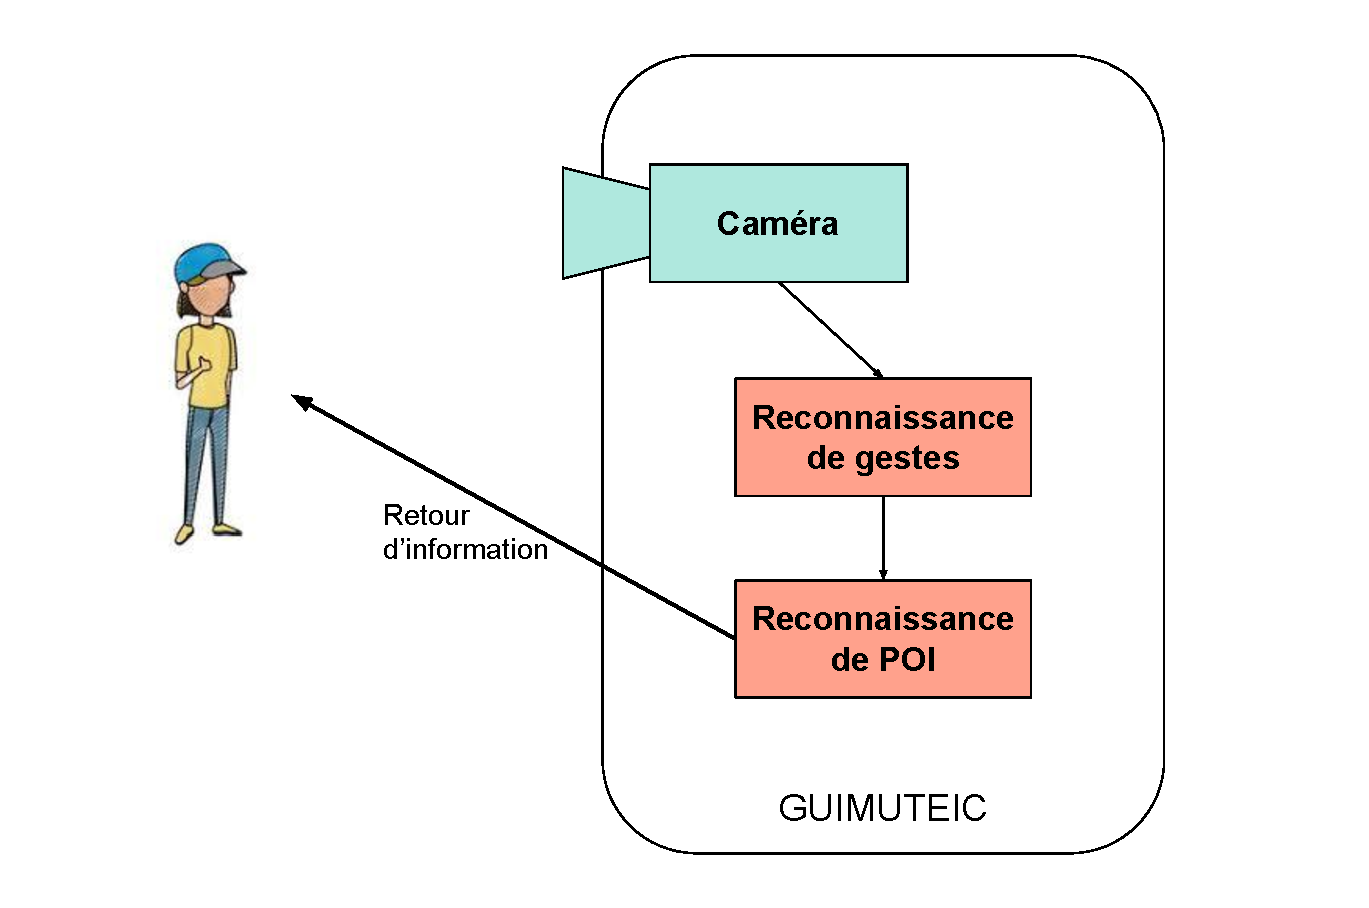
\includegraphics[width=\columnwidth]{figures/Boucledinteraction.pdf}%
\caption{Schéma d'organisation du système d'information GUIMUTEIC.}%
\label{fig:actioncontexte}%
\end{figure}



\begin{savequote}[75mm] 
Objets inanimés, avez-vous donc une âme?
\qauthor{Larmartine} 
\end{savequote}

\chapter{État de l'art}
\label{chap:stateoftheart}

\section{Caractéristiques ingéniérées}
\label{sec:stateoftheartingenierees}


\section{Apprentissage automatique à base de réseau de neurones convolutionels}
\label{sec:stateoftheartNN}


\section{Apprentissage automatique à base de réseau de neurones convolutionels}
\label{sec:stateoftheartNN}

\section{Réseau siamois}
\label{sec:stateoftheartsiamois}





\begin{figure}
	\centering
    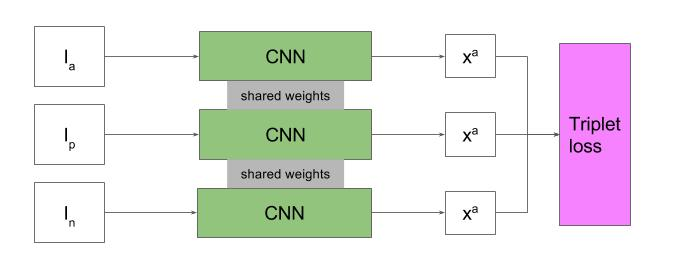
\includegraphics[width=\linewidth]{figures/3way_siamese__1_.jpg}
    \caption{Siamese Architecture use to train a network (NN) with a triplet of images, with an anchor image (a), a negative image (n) and a positive image (p)
    \label{fig:tripletloss}}
\end{figure}




%
%\section{Les visites augmentées}
%
%Système existant.
%Manière de tracker.
%
%
%\section{Instance, classe et identification}
%
%Difference entre recherche d'instance et classification
%Rechercher les travaux theorique sur la représentation d'instance.
%
%
%\section{Corpus d'images muséales}
%
%Il existe des collections sur des données muséales, comme le challenge du musée Rijk~\cite{mensink2014rijksmuseum}, qui propose plus de 110 000 œuvres artistiques du XIX$^{\text{\`e}me}$ siècle, ou le BNF Benchmark~\cite{picard2015challenges}. Cependant, ces corpus ne proposent qu'une seule image par œuvre et pas de requêtes adaptées à la recherche d'instances. Dans notre cas, plusieurs images par œuvre sont présentes et nous avons défini des requêtes associées. De plus, ces images ont des proportions variables d'arrière-plan, et sont prises de différentes perspectives.
%
%Les corpus d'images pour la recherche de catégorie d'objets (comme VOC 2007~\cite{Everingham2010} par exemple), ne sont pas adaptés à la recherche d'instance qui nous intéresse ici. La collection de la tâche {\it instance search} de TRECVid 2013\footnote{http://www-nlpir.nist.gov/projects/tv2013/tv2013.html\#ins} s'intéresse à des recherches d'instances, mais son corpus est uniquement composé de vidéos, ce qui sort du cadre de notre étude. Les caractéristiques des corpus qui se rapprochent des nôtres pour la recherche d'images au niveau instances sont à, notre connaissance, les suivants:
%\begin{itemize}
%\item Oxford Buildings\footnote{http://www.robots.ox.ac.uk/~vgg/data/oxbuildings/}: 5062 images, 55 requêtes, composée d'images représentant des bâtiments d'Oxford. Il y a 17 bâtiments différents, ce qui limite l'attrait pour la recherche d'instance. Ce corpus indique explicitement les images qui  portent partiellement sur un objet, ce qui peut permettre de mesurer la robustesse d'une approche. Des résultats publiés en 2015~\cite{Chatfield2015}  obtiennent des scores de MAP de 0.89, en concaténant cette collection avec un ensemble de 100 000 autres images tirées de Flickr, ce qui nous fait dire que cette collection n'est pas très difficile avec des approches de l'état de l'art;
%\item Holidays: 1491 images, 500 requêtes (scènes), composés d'images de vacances. Ce corpus contient quelques images par scène, et ne contient que des images en extérieur;
%\item Paris6k\footnote{http://www.robots.ox.ac.uk/~vgg/data/parisbuildings/}: 6412 images, avec des images de bâtiments parisiens. Ces images sont tirées de Flickr, donc peu contrôlées. Les autres caractéristiques sont similaires à Oxford5k;
%\item Sculpture6k\footnote{http://www.robots.ox.ac.uk/~vgg/data/sculptures6k/}: 6340 images (3170 de train et 3170 de test pour vérifier les modèles appris), 70 requêtes. Ce corpus est composé d'images de sculptures de Rodin et Moore. Les résultats reportés en 2011~\cite{Chatfield2015} par les auteurs de la collection donnent une MAP de 0,50, ce qui n'est pas très élevé. On peut donc considérer que cette collection est difficile, en particulier à cause de la nature 3D des œuvres considérées.
%\end{itemize}
%
%Le tableau~\ref{tab:exist_corpus} présente une description des collections ci-dessus dans le cadre de notre analyse de paramètres des collections.
%
%\begin{table}[htb]
%    \centering
%    \begin{tabular}{| c || c | c | c | c |}
%    \hline 
%    & Oxford5k & Holidays & Paris5k & Sculpture6k \\
%    \hline \hline
%    objet & bâtiments (3D) & scènes (3D) & bâtiments (3D) & œuvres (3D) \\
%    \hline 
%    support & Image & Image & Image & Image \\
%    \hline
%    acquisition & Flickr &  Flickr & Flickr & Flickr \\
%    \hline
%    taille (C/Q) &  5052 / 55 & 1491 / 500 & 6412 / 12& 6340 / 70\\
%    \hline
%    \end{tabular}
%    \caption{Caractéristiques des collections existantes}
%    \label{tab:exist_corpus}
%\end{table}
%
%Nous en concluons qu'il n'existe pas à notre connaissance de corpus d'objets de musées capables de représenter une certaine variabilité des objets (2D et 3D) et des supports (images ou vidéos), tout en garantissant un grand nombre d'images par objet recherché.
%
%
%\section{Descripteurs visuels locaux}
%
%Présenter les évolutions des descripteurs visuels.
%Ouvrir sur les réseaux de neurones
%
%
%\section{Réseaux de neurones à convolutions}
%
%Introduction au réseau de neurones.
%Comment on entraine une réseaux.
%Le besoin de données
%Les réseaux qui marchent le mieux.
%
%
%\section{Recherche d'instance à base de descripteurs visuels}
%Before the ground-breaking results of deep learning methods for object dection, and image retrieval, shallow descriptors like SIFT~\cite{lowe2004distinctive} have been used. Inspired by text retrieval methods like bag of words~\cite{barroso2003web}, methods used bag-of-features image representation~\cite{sivic2003video}. Each image is represented by a bag-of-features (BoF), with SIFT features clustered as vocabulary. For image retrieval, a inverted file structure~\cite{witten1999managing} is used to allow fast retrieval. An image is retrieved by computing its vector of visual words, and finding the closest one (by cosine distance).
%Aggregated descriptors like VLAD~\cite{jegou2010aggregating} are an evolution of BoF, with smaller vocabulary, more adapted to large dataset.
%The advantage of these methods is that they are compatible with query expansion. Query extension improve performance of retrieval system~\cite{arandjelovic2012three}, ranking image for a given region by tf-idf, and averaging BoF corresponding to the region visual words with the query BoF.
%
%\section{Methodes à base de réseaux de neurones}
%
%Plus grosse partie normalement.
%Aller de l'extraction de features à Gordo.
%
%After the success of CNN for classification, they have been used for several tasks, including image retrieval, with solid performances. 
%The first and trivial approach is to use CNN as features generator. A state-of-the-art large CNN is trained on an unrelated image classification dataset (e.g. ImageNet~\cite{deng2009imagenet}).
%This CNN is then to generated image representation~\cite{sharif2014cnn, babenko2014neural}. For image retrieval, the distance between the query image and collection images is performed to evaluate similarity.
%These methods outperformed standard descriptor approaches, but stay below the state of the art. 
%\begin{savequote}[75mm] 
%Nulla facilisi. In vel sem. Morbi id urna in diam dignissim feugiat. Proin molestie tortor eu velit. Aliquam erat volutpat. Nullam ultrices, diam tempus vulputate egestas, eros pede varius leo.
%\qauthor{Quoteauthor Lastname} 
%\end{savequote}

\chapter{Identification d'œuvres}
\label{chap:similarite}
%%%%%%%%%%%%%%%%%%%%%%%%%%%%%%%%%%%%%%%%%%%%%%%%%%%%%%%%%
%														%
%		INTRODUCTION									%
%														%
%%%%%%%%%%%%%%%%%%%%%%%%%%%%%%%%%%%%%%%%%%%%%%%%%%%%%%%%%

Comme énoncé précédemment, le système GUIMUTEIC doit être capable de reconnaître l'environnement de l'utilisateur afin de lui donner les informations qu'il désire sur ce qui l'entoure.
Pour identifier cet environnement, nous nous basons sur la reconnaissance d'œuvres, ou instances, et de points d'intérêts. 
Cette reconnaissance d'instances, présentée dans la chapitre~\ref{chap:stateoftheart}, peut être faite par recherche d'images. 
Ce chapitre étudie le problème de reconnaissance d'instances dans les images. 
Notre approche, basée sur l'apprentissage de similarité entre les images, repose sur les réseaux de neurones profonds de type siamois à trois branches.




%%%%%%%%%%%%%%%%%%%%%%%%%%%%%%%%%%%%%%%%%%%%%%%%%%%%%%%%%
%														%
%		SIMILARITE										%
%														%
%%%%%%%%%%%%%%%%%%%%%%%%%%%%%%%%%%%%%%%%%%%%%%%%%%%%%%%%%
\section{Similarité entre les images}
\label{sec:similarite}
Le reconnaissance d'instances consiste à identifier, sur une image donnée, le ou les objets présents. 
Elle se distingue de la classification d'images, dans le sens où on ne s'intéresse pas à une catégorie d'objet, mais à un objet bien identifié. 
Longtemps basé sur les comparaisons d'images à l'aide d'extraction de caractéristiques visuels sur celles-ci, l'utilisation d'apprentissage automatique donne aujourd'hui les meilleurs résultats, comme montré dans le chapitre~\ref{chap:stateoftheart}.

La reconnaissance d'instances peut se faire à l'aide de recherche d'images, où l'on cherche dans une base de données les images les plus ``ressemblantes'', pour déterminer quel objet est visible sur l'image. 
Cette tâche revient donc à déterminer ce qu'est la ressemblance entre deux images. 
Dans notre cas, similarité signifie avoir la même instance. 
Dans le cas idéal, nous souhaiterions avoir la fonction similarité $S$ définie par:

\begin{equation}
S(I_1, I_2) = 
  \begin{cases}
   1       & \quad \text{si } I_1 \text{ et } I_2 \text{ contiennent le même objet}\\
   0  & \quad \text{ sinon }
  \end{cases}
\label{eq:similarite}
\end{equation}

Dans la suite de ce chapitre, le but sera d'approximer cette fonction S.
Une fonction approximée de S tend vers 1 si les images sont similaires.
Pour déterminer l'objet présent dans les images, nous retrouvons les images similaires dans la base de données. 
Comme montré sur le schéma~\ref{fig:rechercheimage}, la recherche d'image permet de classer les images, et ainsi définir la fonction de similarité en fonction de score de ressemblance entre les images.


\begin{figure}%
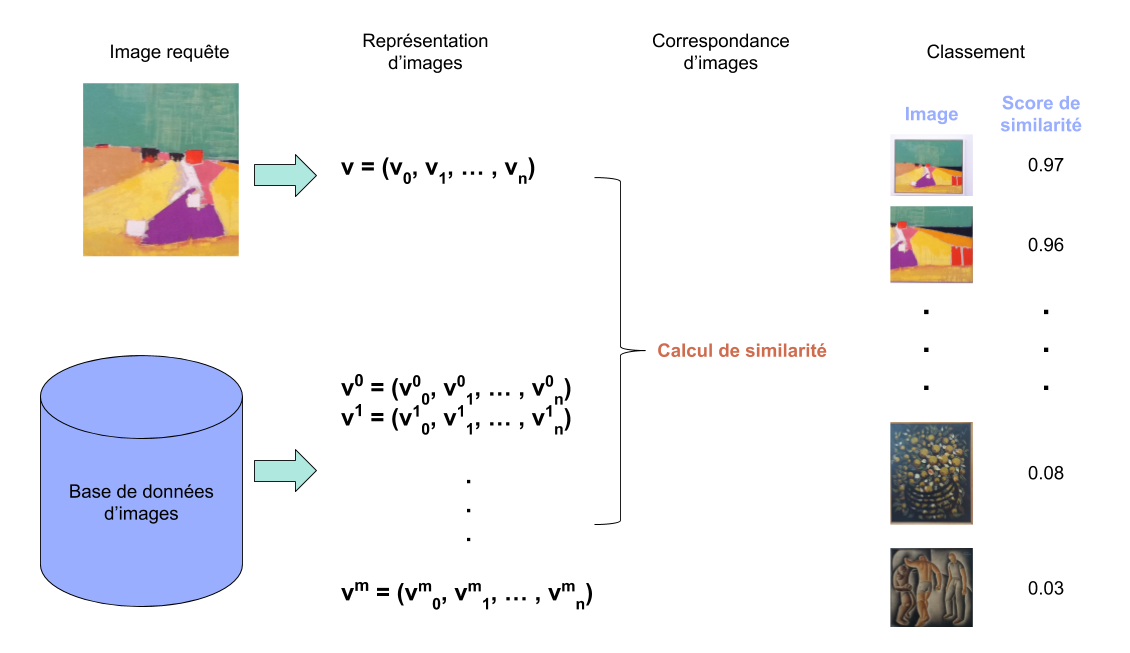
\includegraphics[width=\columnwidth]{figures/rechercheimage.png}%
\caption{Exemple fictif de recherche d'image par le contenu. Le classement représente la similarité entre les images.}%
\label{fig:rechercheimage}%
\end{figure}
 
Nous voyons sur le schéma~\ref{fig:rechercheimage} que pour calculer la similarité des images, nous avons besoin de créer une représentation commune des images $V$. Nous avons exploré dans le chapitre~\ref{chap:stateoftheart} différents moyens de créer ses représentations, à l'aide de descripteurs visuels, ou par apprentissage automatique. En ce basant sur cet état de l'art, il apparait que les méthodes à base de réseaux de neurones profonds, notamment grâce aux réseaux siamois, permettent les meilleurs résulats. 

 
\section{Représentation d'image et similarité}

Pour comparer les images, celles-ci doivent avoir une représentation commune qui permet un calcul de similarité.
Pour créer une représentation commune des images, nous créons un espace de projection de dimension $N$, où chaque images est représentée par un vecteur $V$, son plongement.
La caractéristique principale de cet espace est que les distances entre les vecteurs doivent être inversement proportionnelles à la similarité entre les images. 
La distance entre entre $V_1$ et $V_2$ doit être minimale si l'image $1$ et l'image $2$ représentent le même objet.
Comme montré sur le schéma~\ref{fig:imagespace}, le plongement dans cet espace doit regrouper les images similaires ensemble, et les éloignées des autres. 
Ainsi, en projetant l'image requête dans cette espace, nous pouvons déterminer l'objet présent dans celle-ci, à l’aide de la recherche du plus proche voisin.

\begin{figure}
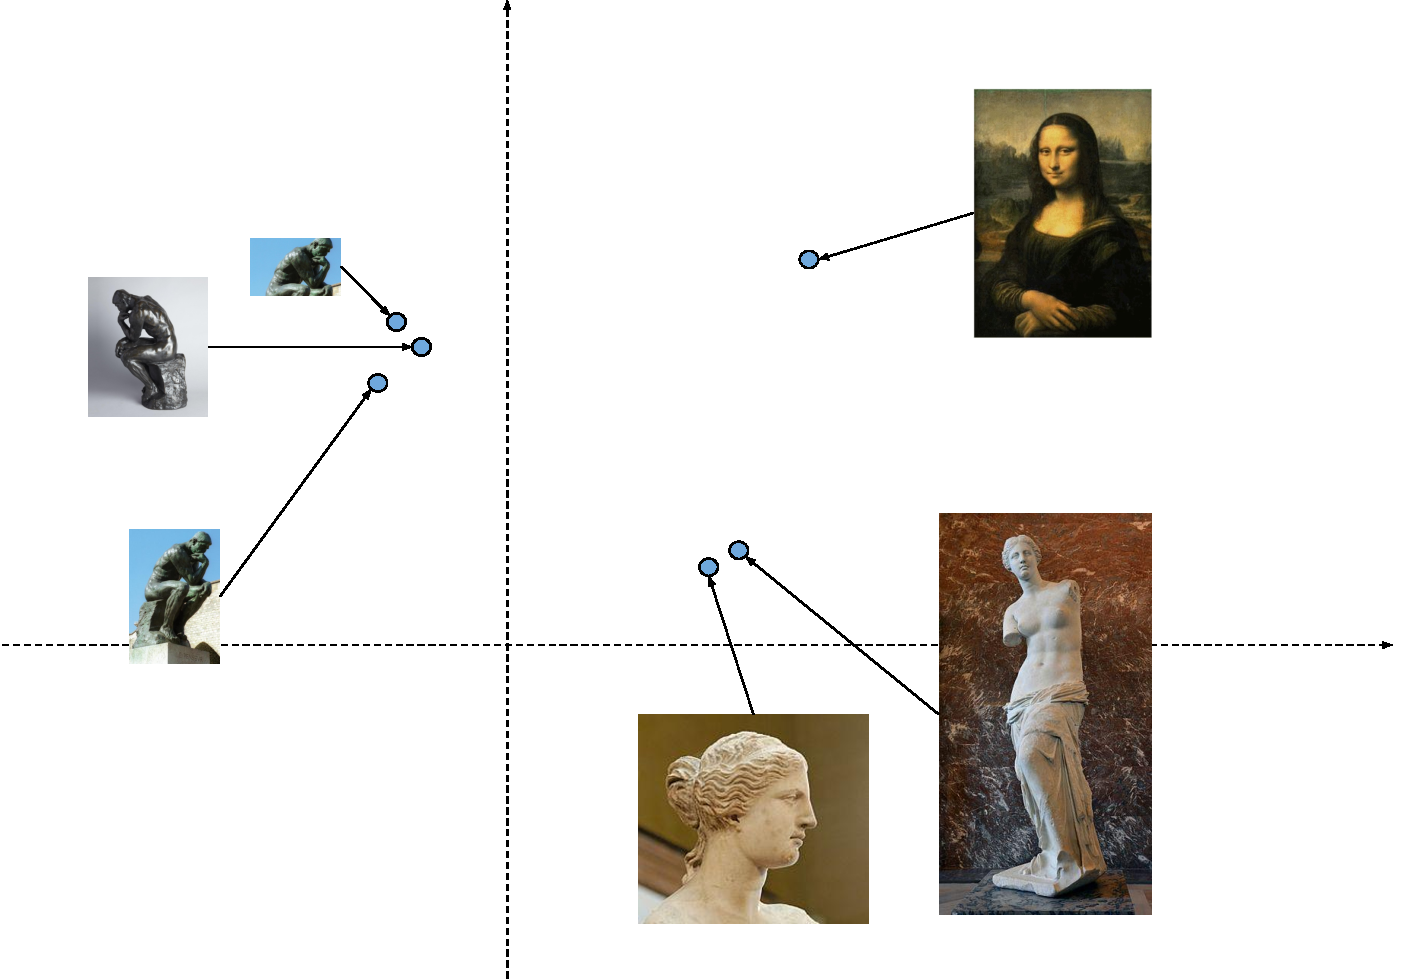
\includegraphics[width=\columnwidth]{figures/imagespace.pdf}
\caption{Projection d’images dans un plan 2D}
\label{fig:imagespace}
\end{figure}


La dimension $N$ de l'espace de projection a une forte importance dans notre contexte. Cette dimension va déterminer une partie du temps de recherche des images. Plus cette dimension est grande, plus les temps de calcul seront important. De la même manière, le type de métriques utilisé pour le calcul de similarité va impacter le coût de calcul. 
L'avantage d'utiliser une méthode d'apprentissage automatique, est que nous pouvons établir la fonction objectif de l'apprentissage en fonction de la métrique qui nous intéresse. 


\section{Plongement des images}

Nous souhaitons apprendre une projection des images, un plongement, qui capture la similarité entre les images. 
Pour le construire, nous utilisons un réseau de neurones, dont la sortie est la projection de dimension $N$. 
Nous avons montré dans le schéma~\ref{fig:extractfeatures} de la section~\ref{sec:extractfeatures} qu'il est possible d'extraire les caractéristiques depuis n'importe quelle couche cachée d'un réseau de neurones pour créer un représentant de l'image. 
Dans notre cas, nous voulons créer un plongement $V \in \mathbb{E}$ qui projette l'image dans un espace euclidien $\mathbb{E}$ de dimension $N$.

Nous créons un réseaux de neurones qui produit le plongement $P$ des images.
Pour l'apprentissage de ce réseau, nous nous basons sur la seule information dont nous disposons, c'est-à-dire un ensemble d'images avec leur étiquette pour savoir si elles représentent le même objet. 
Etant donnée une image $I$ parmi l'ensemble des images disponibles $\tau$, nous définissons l'ensemble des images $\tau_p(I)$ contenant le même objet que l'image $I$ (équation~\ref{eq:pi}), et inversement $\tau_n(I)$ l'ensemble des images ne contenant pas le même objet que $I$ (équation~\ref{eq:ni}).

\begin{equation}
\tau_p(I) = \left\{ x \in \tau | S(I, x) = 1 \right\}
\label{eq:pi}
\end{equation}

\begin{equation}
\tau_n(I) = \left\{ x \in \tau | S(I, x) = 0 \right\}
\label{eq:ni}
\end{equation}



\section{Réseau siamois}

Dans le chapitre~\ref{chap:stateoftheart}, nous avons détaillé l'apprentissage à base de réseaux siamois. 
Ces derniers permettent d'apprendre une similarité entre les images~\cite{schroff2015facenet}. 
Nous nous basons sur les réseaux siamois à trois branches, présentés sur le schéma~\ref{fig:tripletloss}.
Ceux-ci obtiennent les meilleures performances pour la recherche d'instance~\cite{gordo2016deep}, et sont plus adaptés pour les collections de taille réduite.


Là où Schroff et al.~\cite{schroff2015facenet} peuvent se baser sur une grande collection d'image de visage pour apprendre les différences, nous ne disposons pas de corpus aussi important pour la recherche muséale. 
Pour être capable d'utiliser des réseaux profonds de grandes tailles, qui fournissent généralement les meilleures résultats, nous devons utiliser du transfert de connaissances (présenté en section~\ref{sec:transfertlearning}). 
Comme nous allons réaliser une première partie de l'apprentissage sur ImageNet~\cite{deng2009imagenet}, nous basons donc notre architecture sur des réseaux convolutionnels qui sont capables d'obtenir de bonnes performances sur cette collection.
Une fois l'apprentissage réalisé sur ce corpus, nous pouvons spécialiser notre réseaux pour créer le plongements $P$ qui nous intéressent.
Cette phase d'apprentissage se fait à l'aide de triplets d'images.
Ces triplets représentent (équation~\ref{eq:triplets}) une image de \textbf{référence}  $I_r$, une image \textbf{positive}  $I_p$ représentant le même objet que l'image référence, et une image \textbf{négative}  $I_n$ qui contient un objet différent.

\begin{equation}
\Eta = \left\{ (x,y,z) \in \tau^3 | y \in \tau_p(x) \text{ et } z \in \tau_n(x) \right\}
\label{eq:triplets}
\end{equation}

\begin{figure}%
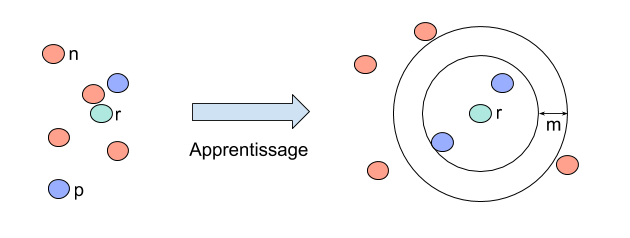
\includegraphics[width=\columnwidth]{figures/Entrainementtriplet.png}%
\caption{Schéma de l'apprentissage du plongement des images, pour une image de références r, avec les images positives p représentant le même objet, et les images n qui contiennent des objets différents.}%
\label{fig:apprentissagetriplet}%
\end{figure}

Le réseau de neurones produit une fonction $P$ de plongement des images dans $\mathbb{E}$. Pour entraîner ce réseau, nous devons définir une \textbf{fonction objectif} associée. 
Cette fonction doit capturer la similarité entre les images.
Nous voulons que $P(I_r)$ soit plus proche du plongement $P(I_p)$ que de $P(I_n)$, comme montré par l'équation~\ref{eq:objectif}, avec $m$ qui représente la marge minimale désirée entre les plongements positifs et négatifs :

\begin{equation}
\forall (x,y,z) \in \Eta, ||x - y|| + m < ||x - z|| 
\label{eq:objectif}
\end{equation}

Cette marge $m$ nous permet de définir un seuil, qui nous permet de déterminer la similarité $S$:

\begin{equation}
S(I_1, I_2) = 
  \begin{cases}
   1       & \quad \text{si } || P(I_1) - P(I_2) || < m\\
   0  & \quad \text{ sinon }
  \end{cases} 
\label{eq:simmargin}
\end{equation}



Nous nous intéressons uniquement à la projection sur l'hypersphère unité des plongements (equation~\ref{eq:hypersphere}). 
Ce qui permet d'utiliser le produit scalaire uniquement pour calculer la similarité cosinus entre les embeddings et mène à un calcul de gradient moins coûteux.
\begin{equation}
\forall I \in \tau, P(I) = \frac{P(I)}{||P(I)||},\text{ donc }||P(I)|| = 1
\label{eq:hypersphere}
\end{equation}
 

Pour l'apprentissage, nous souhaitons donc à minimiser l'équation \textbf{objectif triple}:

\begin{equation}
\mathcal{L}(x,y,z) =  \max(0, P(x) \cdot P(z) - P(x) \cdot P(y) + m)
\label{eq:losstriple}
\end{equation}

pour l'ensemble des triplets $(x,y,z) \in \Eta$. 
Cette fonction de coût est grande si $z$ est similaire à $x$, autrement dit elle est proportionnelle au produit scalaire $P(x)\cdot P(z)$.
Et elle diminue si $y$ est similaire à $x$, c'est-à-dire qu'elle est inversement proportionnelle à $P(x)\cdot P(y)$.
Ce qui correspond sur le schéma~\ref{fig:apprentissagetriplet}, à éloigner les exemples négatifs et rapprocher les exemples positifs pendant l'entrainement.
La fonction $P$ produite par le réseau de neurones doit donc faire tendre la fonction objectif triple vers 0.




\section{Choix des triplets}

Lorsque l'on utilise une fonction objectif triple il faut être particulièrement attentif à la sélection des triplets~\cite{schroff2015facenet}. 
La qualité de l'apprentissage et la vitesse de convergence vont dépendre des triplets présentés au réseau pendant l'apprentissage.
Plus précisément, il existe des exemples plus ou moins ``faciles''.
Il nous faut choisir les triplets pour l'apprentissage pour deux principales raisons : un triplet facile ne fait rien apprendre au réseau et des triplets trop difficiles dès le départ conduisent rapidement à un minimum local ou font s'effondrer le réseau ($P(x) = 0, \forall x$).

Un exemple facile, à gauche sur le schéma~\ref{fig:exemplefacile} correspond à un triplets où les projections sont correctes. Au centre, un exemple difficile correspond au cas où le plongement de l'image négative est plus proche de l'image de référence que celui de l'image positive, et comprend également tous les cas où l’ordre entre positif et négatif n’est pas respecté. Enfin, nous référons à un exemple semi-difficile, à droite, dans le cas où les distances entre les embeddings est correcte, mais l'exemple négatif est dans la marge $m$.


\begin{figure}[htbp]

\begin{subfigure}{0.32\textwidth}
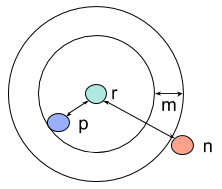
\includegraphics[width=\linewidth]{figures/exemplefaciles.png}
\caption{triplet facile} \label{fig:exemplefacile}
\end{subfigure}
\hspace*{\fill} % separation between the subfigures
\begin{subfigure}{0.32\textwidth}
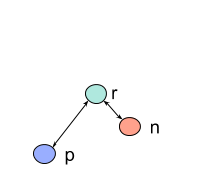
\includegraphics[width=\linewidth]{figures/exempledifficile.png}
\caption{triplet difficile} \label{fig:exempledifficile}
\end{subfigure}
\hspace*{\fill} % separation between the subfigures
\begin{subfigure}{0.32\textwidth}
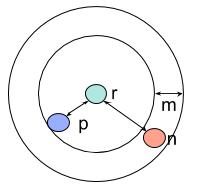
\includegraphics[width=\columnwidth]{figures/exemplesemidifficile.png}
\caption{triplet semi-difficile} \label{fig:exemplesemidifficileb}
\end{subfigure}

\caption{Exemple des différentes configuration des projections possibles. La projection de l'image de référence $r$ est plus ou moins proche des projection de l'image positive $p$ ou de l'image négative $n$.} 
\label{fig:triplets}
\end{figure}




En nous basant sur l'équation~\ref{eq:objectif}, nous pouvons définir un exemple positif facile ou difficile en fonction de la valeur de $||P(x) - P(y)||$ pour un couple d'image $(x,y)$ représentant le même objet. 
Les exemples positifs difficiles $p_d$ sont ceux dont la projection est plus éloignée qu'au moins un des exemples négatifs :

\begin{equation}
p_d(x) = \left\{ y \in \tau_p(x) \middle| \exists z \in \tau_n(x),  \|P(x) - P(y)\| > \|P(x) - P(z)\| \right\}
%p_d = \argmax_{y \in \tau_p(x)} ||P(x) - P(y)||
\label{eq:maxhard}
\end{equation}

Nous définissons de la même manière les exemples négatifs difficiles $n_d$ en fonction de la valeur de $||P(x) - P(z)||$, où les images $x$ et $z$ représentent des objets différents: 

\begin{equation}
n_d(x) = \left\{ z \in \tau_n(x) \middle| \exists y \in \tau_p(x),  \|P(x) - P(y)\| > \|P(x) - P(z)\| \right\}
%n_d = \argmin_{z \in \tau_n(x)} ||P(x) - P(z)||
\label{eq:minhard}
\end{equation}

L'ensemble les \textbf{triplets difficiles} $\Eta_d$ (équation~\ref{eq:hardtriplet}) correspond aux triplets pour lesquels les exemples positifs et négatifs sont diffiles.

\begin{equation}
\Eta_d = \left\{ (x,y,z) \in \Eta \middle| y \in p_d(x) \text{ et } z \in n_d(x) \right\}
\label{eq:hardtriplet}
\end{equation}

Une première stratégie pour la selection des triplets, proposée par Schroff et al.~\cite{schroff2015facenet}, consiste à prendre les triplets semi-difficles, en choisissant les positifs les plus difficiles, et de prendre les exemple négatifs qui sont dans la marges $m$.
Une autre méthode par Gordo et al.~\cite{gordo2016deep}, propose de choisir les $i$ exemples positifs les plus faciles et les $j$ négatifs les plus difficiles, de choisir parmis toutes les combinaisons possibles de triplets celui qui maximise la fonction objectif triple. 
Ce choix semble très pertinent, car il permet de déterminer les exemples qui feront converger le plus rapidement, tout en élimant les images positifs difficiles, c'est-à-dire celles qui représentent la même instance, mais avec trop de différences visuelles. 
Cette méthode demande cependant de parcourir l'ensemble des données d'apprentissage pour calculer la fonction de coût.
Comme le réseau est mis à jour à chaque rétro-propagation, il faut recalculer la fonction de coût assez fréquemment.

Avec nos contraintes spécifiques, à savoir surtout que nous ne disposons que d'un ensemble limité d'exemples positifs, nous choisissons une méthode de selection des triplets hybride entre les deux présentée précédemment. 
Nous choississons l'ensemble des triplets $\Eta_{sd}$, où pour l'ensemble des couples positifs possibles, nous choississons les exemples négatifs semi-difficiles :
\begin{equation}
\Eta_{sd} = \left\{ (x,y,z) \in \Eta \middle| \|P(x) - P(y)\| < \|P(x) - P(z)\| < \|P(x) - P(y)\| + m \right\}
\label{eq:semihardtriplets}
\end{equation}

La figure~\ref{fig:pipelinesimilarite} montre les étapes de l'apprentissage du réseau.
Dans un premier temps, le réseau est appris sur une base de données de grande taille, par exemple ImageNet.
La deuxième étape correspond en un fine-tuning sur la collection du musée.
Ceci permet de spécifier le réseau aux images de musée, étant donné la différence entre les deux collection, ce qui rend la convergence à l'étape suivante plus rapide.
Finalement, nous apprenons le réseau à l'aide des triplets d'image du musée.


Dans un second temps, une fois qu'il n'y a plus de convergence, nous choisissons tous les triplets de $\Eta_d$.

\begin{figure}[htbp]
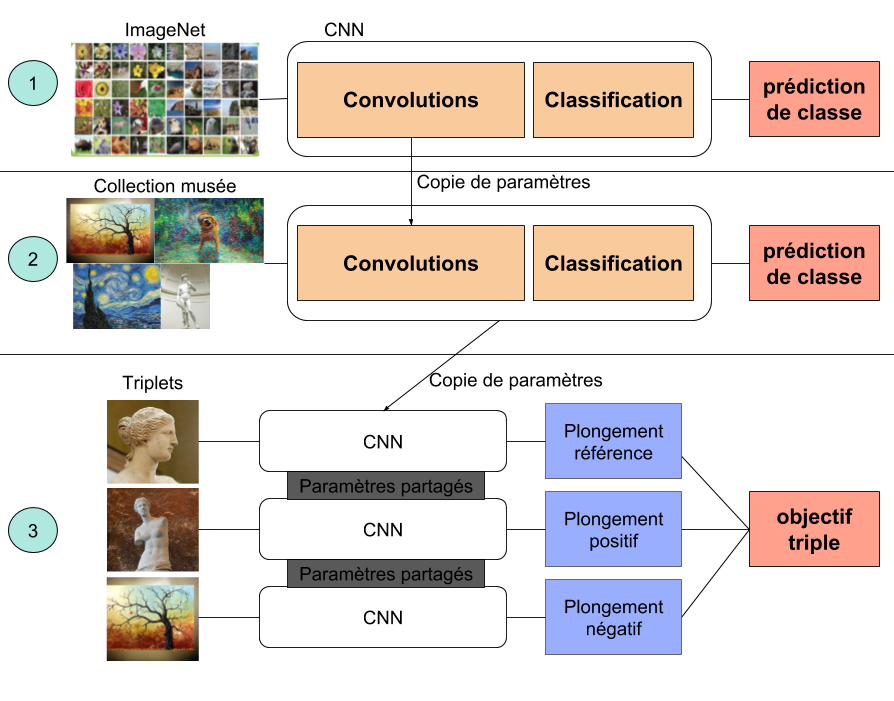
\includegraphics[width=\columnwidth]{figures/pipeline1.png}%
\caption{Pipeline d'apprentissage. L'étape 1 correspond à l'apprentissage du réseau sur une grande collection d'image, ici ImageNet. L'étape 2 est le fine-tuning sur la collection du musée. La troisième étape consiste à apprendre à l'aide du réseau siamois triple.}%
\label{fig:pipelinesimilarite}%
\end{figure}



\section{Évaluation}

Pour évaluer notre première proposition, nous utilisons la collection CLICIDE (détaillée dans la section~\ref{sec:garofou}). 
Ce corpus représente un ensemble de photos d'un musée d'art, et donc surtout des tableaux et peintures, avec différents points de vue sur les oeuvres, et correspond aux contraintes lié à notre projet. La collection GaRoFou (section~\ref{sec:garofou}) vient du musée d'archéologie de Lyon Fourvière, et présente des objets de différentes natures, comme des sculptures, des artéfacts ou des stèles.

Nous comparons notre approche à celles de l'état de l'art, et à diverses méthodes de deep learning. 
Les méthodes à base de descripteurs visuels sur ce dataset ont été explorées précédemment~\cite{portaz2017construction}, avec l’utilisation de SIFT et de sacs de mots visuels. 
Pour identifier l'image similaire dans la base d'image qui va nous permettre de déterminer l'objet présent dans l'image, on recherche l'image la plus proche, ce qui correspond au TOP@1 de la recherche d'image :
 
\begin{equation}
TOP@1(I) = \argmin_{x \in \tau} ||P(I) - P(x)||
\label{eq:simrank}
\end{equation}


\subsection{Autres approches comparées}
Toutes les méthodes comparées utilisent le même type d'architectures, à savoir AlexNet et Resnet, présentés plus en détail dans le chapitre~\ref{chap:stateoftheart}. 
Nous nous comparons principalement aux réseaux siamois à trois branches proposés par Gordo et al.~\cite{gordo2016deep}, avec multi-resolution(Gordo multi-res) et sans (Gordo). 
Pour avoir une idée des autres techniques utilisables, nous montrons les résultats obtenus avec:

\begin{itemize}
  \item Extraction de caractéristiques: Alexnet E et Resnet E (pour Extraction). Un réseau de neurones de type Alexnet ou Resnet est appris sur une grande collection, ici Imagenet. 
	Les images du musée sont ensuite représentées par la sortie d'une des couches du réseau. 
	Nous selectionnons ici la couche caché qui donne les meilleurs résultat dans notre cas, à savoir la couche \textit{fc6} pour Alexnet et \textit{pool5} pour Resnet. 
	\item Fine-tuning et classification des oeuvres: Alexnet Classif et Resnet Classif. Un réseau est appris de manière conventionnelle sur ImageNet, et ensuite un apprentissage fin est réalisé où chaque oeuvre est une classe. Les résultats sont ceux de la classification de chaque oeuvres du corpus de test.
	\item Réseau siamois à double branche: Alexnet SS et Resnet SS (pour Siamois Simple). Un réseau siamois à deux branches est utilisé pour l'apprentissage. La selection des couples se fait de la manière suivante : tous les couples positifs possibles, et le même nombre de couple négatifs, qui correspondent aux exemples les plus difficiles. 
\end{itemize}



\subsection{Paramètres d'apprentissages}

Le fine-tuning sur les deux réseaux utilisés se fait en commençant par la dernière couche entièrement connectée.
Nous apprenons tout d'abord la dernière couche seule, et après stabilisation de la fonction de coût, nous ajoutons à l'entraînement la couche précédente.
Nous continuons ainsi jusqu'à avoir entraîné toutes les couches.
Il est important de ne pas entraîner tous les réseaux d'un seul coup, car lorsque l'on fait un \textit{fine-tuning}, on supprime la dernière couche de classification pour la remplacer par une qui a le bon nombre de sorties.
Cette nouvelle couche étant initialisé aléatoirement, l'erreur de classification sera grande, et propager cette erreur risque de détruire l'ensemble du réseau.
Il est donc nécessaire de procéder couche par couche, car les premières couches sont moins susceptible de devoir être changée, étant donné qu'elles capturent des caractéristiques de plus bas niveau, plus proche de l'image.
De plus, entraîner tout le réseau sur une petite collection entraine un sur-apprentissage, les premières couches ne devraient donc pas être modifiée.

Ces considérations mènent à l'apprentissage suivant:

\begin{itemize}
	\item Pour AlexNet : apprentissage depuis la dernière couche jusqu'à la dernière couche convolutionnelle. Les premières couches convolutifs ne sont pas modifiées.
	\item Pour ResNet : apprentissage de deux dernier bloc de convolution. Contrairement à AlexNet, ResNet repose sur moins de couches entièrement connectées, nous devons donc entraîner davantage de couches convolutionnelles. Comme cette architecture est basé sur des blocs de convolution, nous nous référons à un bloc en entier.
\end{itemize}


\subsection{Etude de l'importance de l'augmentation de données d'apprentissage}
\label{subsec:dataaug}

Toutes les approches présentées se basent sur un fine-tuning.
L'apprentissage sur le corpus de départ, ainsi que sur notre collection, est fait avec une partie d'augmentation de données.
Cette augmentation consiste en différentes perturbations faites sur les images pour éviter un sur-apprentissage du réseau.
Autrement dit, si notre réseau sur-apprend, il aura une capacité limitée à s'adapter à des données différentes de celle d'apprentissage.
Comme nous nous basons sur du transfert de connaissance pour être capable de travailler sur nos collections de petites tailles, cette généralisation est un élément important de notre pipeline.

L'augmentation de données a deux objectifs.
Le premier est d'augmenter le nombre de données présentées au réseau de neurones.
La performance des réseaux de neurones est très fortement liée à la quantité de données sur laquelle on travaille.
Particulièrement dans notre cas, cette augmentation nous permet d'éviter un sur-apprentissage très prononcés sur les petites collections.
Le deuxième objectif est de pallier au manque de variation dans les images de la base d'entrainement. 
En simulant des déplacement de caméra, d'effet de zone, de rotation, on aide le réseau à être invariant à ces transformations.
Trois différentes transformations d'images sont aléatoirement appliquées pendant l'entrainement:


\begin{itemize}
	\item Rotation des images avec une probabilité équivalente pour tous les angles $\{-180, -90, 0, 90, 180\}$.
	\item Changement d'échelle des images avec un facteur aléatoire pour chaque dimension dans l'interval [0.75, 1.25].
	\item Renversement d'image horizontal avec probabilité de $0.5$
\end{itemize}

Le tableau~\ref{tab:dataaugmentation} présente l'influence de chacune des ces perturbations, avec le réseau ResNet-152.
\begin{table*}
\centering
\begin{tabular}{||c|c|c||c|c||}
\hline 
 \emph{Rotation} & \emph{Scaling} & \emph{Flipping} &
 \multicolumn{2}{c||}{\emph{Mean Precision@1 (in \%)}}\\
\hline 
 \multicolumn{3}{||c||}{} & \emph{CLICIDE} & \emph{GaRoFou}\\
\hline  & & & 72.12 & 92.93\\
\hline  \checkmark  & & & 74.55 & 94.02\\
\hline  & \checkmark & & 76.36 & 93.48\\
\hline  & & \checkmark & 72.12 & 94.57\\
\hline  \checkmark & \checkmark & & 76.97 & 94.57\\
\hline  \checkmark & & \checkmark & 75.75 & 94.57\\
\hline  & \checkmark & \checkmark & 78.18 & 93.48\\
\hline  \checkmark & \checkmark & \checkmark & \textbf{79.39} & \textbf{94.57}\\
\hline
\end{tabular}
\caption{Influence de la rotation, de la mise à l'échelle et du renversement sur les résultats avec l'architecture ResNet-152.
\label{tab:dataaugmentation}}
\end{table*}

Le renversement d'image est particulièrement intéressant dans notre cas. 
Il est souvent utilisé dans l'apprentissage de classe, où l'invariance à l'orientation semble important, dans le cas de reconnaissance d'instance cela semble contre-intuitif.
Notamment dans le cadre de collection de tableaux ou de peintures, nous ne voulons pas confondre deux objets qui pourraient être l'image inversée l'un de l'autre. 
Par exemple, l'oeuvre ``4900 Farben'' (``4900 Colors'')\footnote{https://www.gerhard-richter.com/en/art/microsites/4900-colours} de Gerhard Richter est constituée d'un ensemble de panneaux de carrés de couleurs.
Dans ce cas, le renversement d'une image n'est pas équivalente à l'image d'origine, et ne devrait pas être considéré dans l'apprentissage.

Le tableau~\ref{tab:dataaugmentation} montre que la rotation seule ou la mise à l'échelle seule améliorent les résultats. 
Cependant, comme attendu, le renversement seul n'améliore pas l'apprentissage.
Mais n'importe quelle combinaison de perturbation donne de meilleurs résultat que toute les transformations seules, et ce même en considérant le renversement.
De ces résultats nous pouvons conclure que n'importe quelle augmentation de données à travers des perturbations est toujours utile, même pour la reconnaissance de peinture dans le cadre de la collection CLICIDE.
Pour la collection GaRoFou, n'importe quelle perturbation aide l'apprentissage, mais la combinaison de différente transformations ne change pas les résultats.
Cela peut être dû à la plus grande diversité des objets présents dans la collection, ainsi qu'à leur caractère tri-dimensionnel.


\subsection{Résultats}
\label{sec:resultatsimilarite}

\begin{table*}
\centering
\begin{tabular}{|l|c|}
\hline & {\emph{TOP@1 (in \%)}}\\
\hline & \emph{CLICIDE}\\
\hline \emph{Descripteurs Visuels~\cite{portaz2017construction}} & 70.08\\
\hline \emph{Gordo~\cite{gordo2016deep}} & 90.3 \\
\hline \emph{Gordo multi-res~\cite{gordo2016deep}} & \textbf{92.73} \\
\hline \emph{AlexNet E} & 72.73 \\
\hline \emph{AlexNet Classif} & 78.18 \\
\hline \emph{AlexNet SS} & 75.76 \\
\hline \emph{ResNet E} & 72.12 \\
\hline \emph{ResNet Classif} & 79.39 \\
\hline \emph{ResNet SS} & 85.45 \\
\hline \emph{Architecture AlexNet} & 79.39\\
\hline \emph{Architecture ResNet} & \textbf{92.73}\\
\hline
\end{tabular}
\caption{Évaluation des différentes méthodes d’apprentissage pour la projection des images sur le collection CLICIDE.
\label{tab:resultatssansregion}}
\end{table*}

Tout d'abord, nous pouvons voir sur le tableau~\ref{tab:resultatssansregion} que les méthodes à base de descripteurs visuels ingéniérés sont dépassés par toutes les méthodes à base de réseaux de neurones, même si nous travaillons sur une collection d'image de taille réduite. Pour toutes les méthodes proposés, exception faite de l'extraction de caractéristique, une architecture de type Resnet obtient de meilleurs résultats. Pour l'extraction de caractéristiques depuis un réseau pré-entraîné, il en va de la nature de ces réseaux qui explique que Alexnet ait de meilleures performances. Là où Alexnet est une suite de convolution et de maxpooling, Resnet est une série de bloc avec des skip-connection. Que l'extraction sur une couche donnée donne de moins bons résultats signifie juste que dans ce cas les réseaux de retiennent pas l'information de la même manière. Il est intéressant de noter que malgré la petite taille de la collection et d'un grand manque de diversité dans les images (toutes avec le même fond, dans le même musée, etc), le fine-tuning reste intéressant pour améliorer les résultats.

Nous remarquons surtout que les meilleurs résultats sont obtenu avec notre approche, mais également avec l'approche de Gordo. Bien que ces résultats soient surprenamment haut pour cette approche, car les embeddings ne sont pas appris pour cette collection en particulier, plusieurs arguments peuvent expliquer les de si bon résultats. 
Tout d'abord, le réseau proposer par Gordo est appris sur la collection ..., qui dispose d'un grand nombre d'exemples et d'une grande variabilité, qui se prête donc bien à la généralisation sur un autre corpus. 
Dans cette collection, une forte disparité entre les objets existe, ainsi que de très grand écart de point de vue et de distance de zoom. 
Il n'est donc pas étonnant que les plongements créés soient capables d'exprimer de manière convaincante la similarité entre les images. 
De plus, ce réseau dispose d'une partie de proposition de région d'intérêts. 
Dans le cadre de la recherche d'instance dans les images, la détection de la position de l'objet dans l'image est un élément clef, que nous n'avons pas pour le moment pris en compte dans notre approche. 
Lors de la création de l'embedding de l'image, nous voulons que celui ci représente l'objet présent dans l'image au mieux, en faisant fi du fond, d'autres objets moins visibles, ou du bruit. 

Nous avons proposé une nouvelle fonction objectif, basé sur le produit scalaire, ainsi qu'une nouvelle sélection de triplets, le tout dans un nouveau pipeline d'apprentissage adapté à notre problème, et à nos collections.
Notre proposition obtient des résultats proches de ceux de l'état de l'art, avec un réseau plus simple, sans proposition de région, dû aux limitations d’annotation des collections.
Avoir un réseau capable de détecter les régions d'intérêt, et de créer une représentation uniquement de la région où se situe l'objet semble être un éléments clé pour produire un plongement efficace. 
Dans le chapitre suivant, nous nous intéressons à comment mettre en place un système de détection de régions d'intérêt en plus de ce que nous avons proposé dans ce chapitre.

\chapter{Detection de régions d'intérêts }
\label{chap:regions}

Dans une collection d'images représentant un certains nombre d'objets, les prises de vue peuvent être multiples, de différents angles et à une distance pouvant variée. 
Il devient donc utile de s'intéresser à la position de l'objet dans l'image, que nous appelons région d'intérêt.
Faire un plongement uniquement sur la partie de l'image contenant l'objet permet d'éliminer les autres objets pouvant être présents sur l'image, par exemple des objets à peine visible ou hors mise au point.
Le plongement ainsi réalisé est plus à même de représenter correctement l'objet que le plongement de l'image entière.
Dans le cadre de notre projet, nous ne disposons pas d'annotation des régions d'intérêt dans les images (voir section~\ref{sec:contraintesGUIMUTEIC}). 
Ce chapitre propose une solution pour l'apprentissage de régions d'intérêts dans les images, de manière non supervisé et ne nécessitant pas d'annotation des régions au préalable et donc moins coûteux.

\section{Carte d'activation}

Des solutions à base de réseaux à proposition de régions (RPN pour Region Pooling Network) permettent une proposition automatique des régions par le réseaux. 
Les méthodes de l'état de l'art utilisant ce genre d'approche (section~\ref{sec:rpn}) obtienne une segmentation précise de l'image et une amélioration de la précision des plongements~\cite{gordo2016deep}.
Ces genre de méthodes nécessite toutefois un ensemble d'images annotées avec leurs régions pour fonctionner. 
Nous ne disposons pas d'une base de donnée annotées au niveau des régions. 
Ceci nous amène à développer des solutions ne nécessitant pas la présence de boîtes englobantes dans le corpus d'apprentissage.
Nous avons vu dans la section précédente qu'un apprentissage fin est nécessaire (étape 1 et 2 de la figure~\ref{fig:pipelinesimilarite}).
Ceci ne donne pas en soit des résultat suffisant pour l'identification d'instance, mais permet d'apprendre au réseau une certaine représentation des objets.

Le réseau est entraîné à reconnaître certain objets, et la sortie du réseau est dépendante de la présence ou non de ces objets dans les images.
Il a été montré~\cite{zhou2014object} que lorsqu’un réseau est appris sur une collection, il est capable d’identifier la présence de certains objets, même s’il ne les classifie pas explicitement.
Ce qui signifie que si l’on applique notre réseau sur chaque sous partie de l’image, on obtient des maximum d’activation du réseau, si un des objets qu’il a appris à reconnaître est présent.
On prenant les zones où les réseau a des activations plus importante, on peut créer une carte des activations du réseau.
Ces cartes d’activations sont présentés sur la figure~\ref{fig:heatmaps}.
Un réseau de type ResNet, après un apprentissage fin sur la collection, est appliqué sur un certain nombre de sous partie de l’image.
Les zones en rouge sur les cartes d’activations représentent les endroits où les maximum d’activation était les plus important.
On remarque que ces zones correspondent aux emplacements des objets, avec quelques erreurs sur le troisième tableau.
On voit dans la troisième colonne la classification de chacune de ces sous-partie.
Cette classification n’est pas correcte, avec des labels erronés, et très variés. 
Ces résultats sont en relation avec les résultats relativement faibles obtenu dans le chapitre précédent avec la classification, 79\% contre 92\% pour l’extraction de caractéristiques. 
En revanche, cette méthode permet d'identifier les régions d'intérêt de l'image.

\begin{figure}[!htb]
  \centering
  \begin{minipage}[c]{.33\linewidth}
    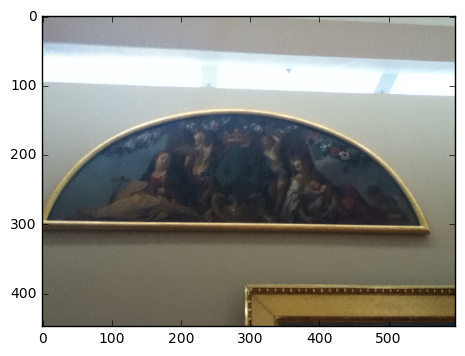
\includegraphics[width=\textwidth]{figures/sample1_10A-0519.png}
    %\caption{Image with label 10A\label{fig:sample1_id}}
  \end{minipage} \hfill
  \begin{minipage}[c]{.33\linewidth}
    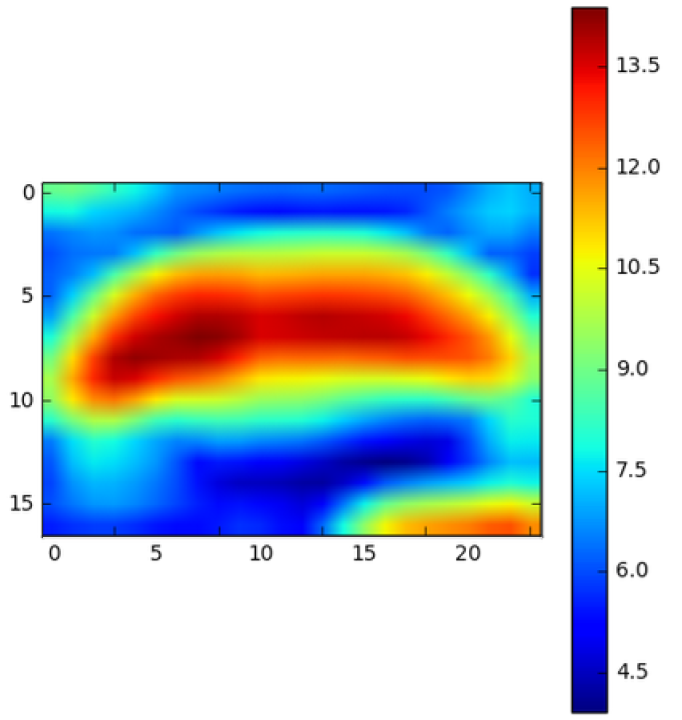
\includegraphics[width=\textwidth]{figures/sample1heatmap.png}
    %\caption{Heat-map for 10A\label{fig:sample1_hm}}
  \end{minipage} \hfill
  \begin{minipage}[c]{.32\linewidth}
    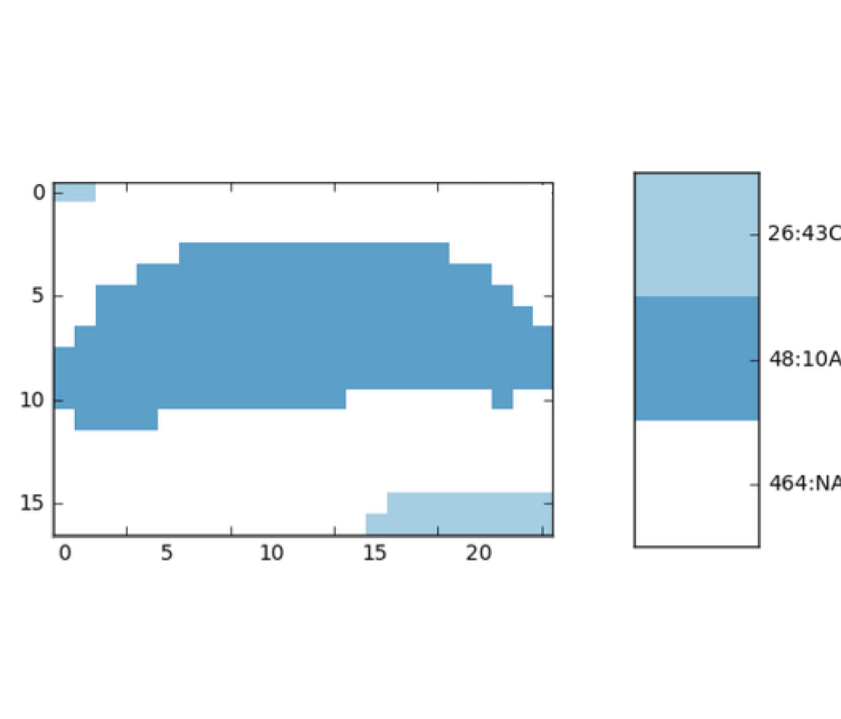
\includegraphics[width=\textwidth]{figures/sample1labels.png}
    %\caption{Label-map for 10A\label{fig:sample1_lab}}
  \end{minipage}

  \begin{minipage}[c]{.33\linewidth}
    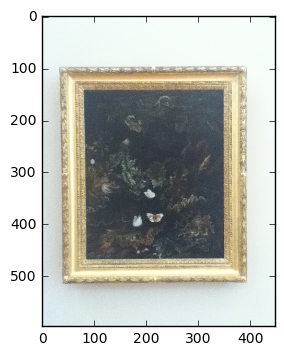
\includegraphics[width=\linewidth]{figures/sample2_5P-0508.png}
    %\caption{Image with label 5P\label{fig:sample2_id}}
  \end{minipage} \hfill
  \begin{minipage}[c]{.33\linewidth}
    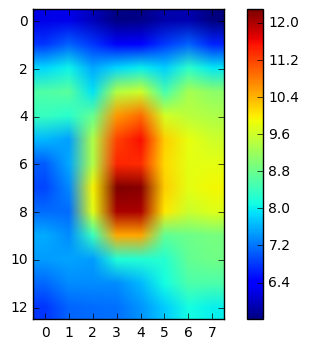
\includegraphics[width=\linewidth]{figures/sample2_heatmap.png}
    %\caption{Heat-map for 5P\label{fig:sample2_hm}}
  \end{minipage} \hfill
  \begin{minipage}[c]{.32\linewidth}
    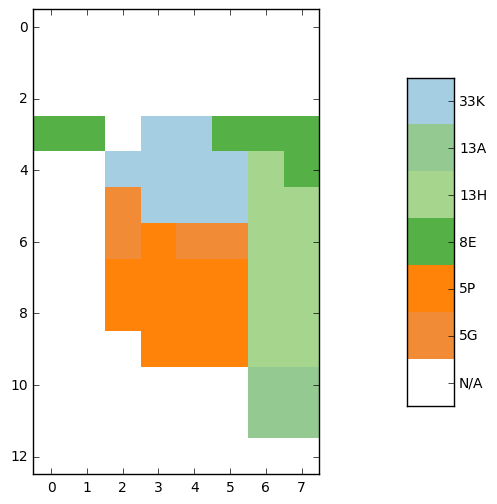
\includegraphics[width=\linewidth]{figures/sample2_labels.png}
    %\caption{Label-map for 5P\label{fig:sample2_lab}}
  \end{minipage}
  
  \begin{minipage}[c]{.33\linewidth}
    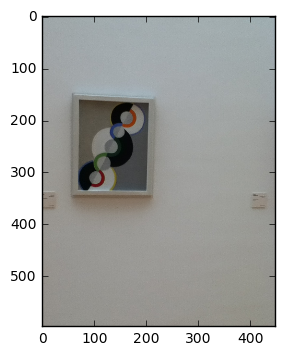
\includegraphics[width=\linewidth]{figures/sample3_30P-0976.png}
    %\caption{Image with label 30P\label{fig:sample3_id}}
  \end{minipage} \hfill
  \begin{minipage}[c]{.33\linewidth}
    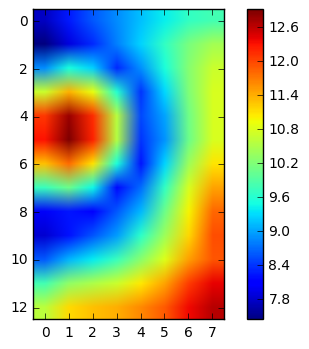
\includegraphics[width=\linewidth]{figures/sample3_heatmap.png}
    %\caption{Heat-map for 30P\label{fig:sample3_hm}}
  \end{minipage} \hfill
  \begin{minipage}[c]{.32\linewidth}
    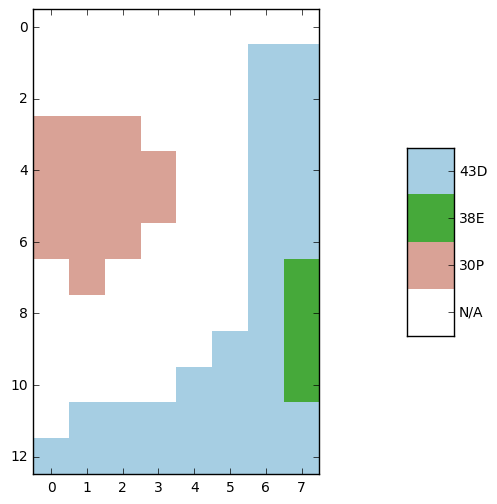
\includegraphics[width=\linewidth]{figures/sample3_labels.png}
    %\caption{Label-map for 30P\label{fig:sample3_lab}}
  \end{minipage}


	\caption{Exemple d'images avec les heat-map des activations maximales, obtenues à partir d'un ResNet-152 après un apprentissage fin. Le réseau est appliqué sur toute l'image de manière strié. Les labels obtenus sur les zones d'activation maximales sont également indiqués.
	\label{fig:heatmaps}}
	
\end{figure}



Le problème avec l'application d'un réseau d’une telle manière est le coût de calcul.
Par exemple, temps de passage d'une image $224*224$ à travers AlexNet est de 1.2 ms. 
Si on applique ce même réseau sur une image $448*448$ avec un pas de 56 pour créer une carte d’activation de $8*8$, il faut 76.8 ms.

Cette méthode n’est donc pas envisageable, surtout s’il on souhaite utiliser des images plus grande pour obtenir une carte d'activation plus précise.
La solution est d’utiliser des réseaux entièrement convolutifs.
Dans la section~\ref{sec:rpn}, nous avons vu que les réseaux entièrement convolutifs pouvaient être utilisés pour la segmentation d'image.
Dans le cas où nous n'avons pas de base données d'apprentissage de la segmentation, nous entraînons le réseau comme expliqué précédemment, et nous remplaçons les couches entièrement connectées par une couche de convolution.
Il y a une équivalence entre une couche entièrement connectée et une couche de convolution $1*1$, comme montré sur le schéma~\ref{fig:equivalencecouche}, avec le même nombre de paramètres.
L'avantage de la couche de convolution est que l'on peut l'appliquer sur n'importe quelle taille d'image (figure~\ref{fig:convBig}), la taille de sortie dépendant de la taille d’entrée.
Le temps d'exécution d’un réseau type AlexNet entièrement convolutionnel sur une image de $448*448$ est de 18 ms, soit 5 fois plus rapide que l’approche naïve.



\begin{figure}[htbp]
\begin{subfigure}{0.32\textwidth}
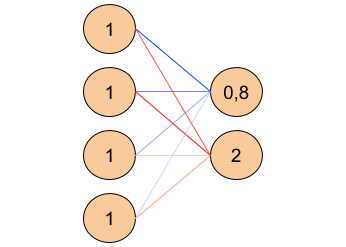
\includegraphics[width=\linewidth]{figures/LinearLayer(1).png}
\caption{Couche Entièrement connectée} \label{fig:linear}
\end{subfigure}
\hspace*{\fill} % separation between the subfigures
\begin{subfigure}{0.32\textwidth}
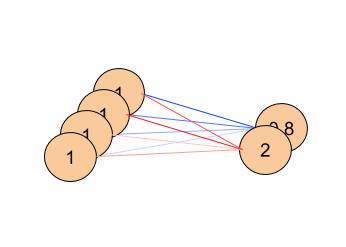
\includegraphics[width=\linewidth]{figures/FConvolutional(1).png}
\caption{Couche de convolution} \label{fig:conv}
\end{subfigure}
\hspace*{\fill} % separation between the subfigures
\begin{subfigure}{0.32\textwidth}
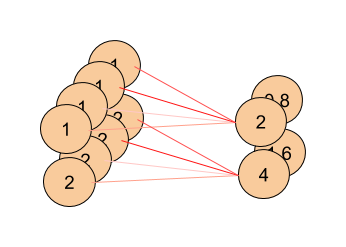
\includegraphics[width=\columnwidth]{figures/FConvolutional2(1).png}
\caption{Même couche de convolution avec entrée plus grande} \label{fig:convBig}
\end{subfigure}
\caption{Exemple d'équivalence entre une couche entièrement connectée et une couche de convolution. Le nombre de paramètres est le même, ici $4*2$, ils peuvent donc être copié pour obtenir les mêmes résultats. On peut appliquer la convolution avec une entrée plus grande, en une seule passe.} 
\label{fig:equivalencecouche}
\end{figure}



\section{Apprentissage sur différentes régions}

L'approche présentée précédemment permet de mettre en avant qu'il est possible de détecter les régions sans apprentissage direct de celles-ci.
Nous pouvons toutefois améliorer les résultats de la détection de régions d'intérêt en faisant un apprentissage fin sur des régions spécifique de l'image, plutôt que sur l'image entière.
En utilisant différentes échelles et différentes régions, toujours pour apprendre la même classe, nous pouvons forcer le réseau à détecter les régions dans l'image.
La fonction de coût associé à cette apprentissage est la moyenne de l'entropie croisée entre les régions et entre les échelles. 
Dans le cas de la classification, l’étiquette d'une image, qui représente sa classe, est un vecteur $\hat{x}$ de dimension $C$, où $C$ est le nombre de classes, où chaque éléments $\hat{x}_i$ est à zéro si la classe $i$ n'est pas présente, $1$ sinon.
La sortie du réseau de neurones $x$ est une distribution de probabilité pour chaque classe.
L'entropie croisée $E$ est définie par :

\begin{equation}
  E(x,\hat{x}) = -\sum_{i=1}^C \hat{x}_i log(x_i)
	\label{eq:entropie2}
\end{equation}

Pour une image à une échelle $s$ donnée, définissons $H_s$ et $W_s$ comme respectivement la hauteur et la largeur de la carte de caractéristiques.
Chaque pixel de la carte d'activation correspond à un sortie du réseau de neurones pour une région de l'image donnée.
Le nombre de région est donc $H_s*W_s$. 
Nous notons $x_{h,w}$ la distribution de probabilité (la sortie du réseau) sur la région $(h,w)$.
Nous définissons la fonction objectif suivante:

\begin{equation}
 \mathcal{L}(x,\hat{x}) = \frac{1}{S} \sum_{s=1}^S \frac{1}{H_s*W_s} \sum_{h=1}^{H_s} \sum_{w=1}^{W_s} E(x_{h,w}, \hat{x}_{h,w})
\label{eq:regionloss}
\end{equation}

qui représente la moyenne de l'entropie croisée de l'ensemble des régions, moyennée sur l'ensemble des échelles de l'image.
La figure~\ref{fig:regionfinetuning} représente l'apprentissage avec cette fonction objectif. 
L'idée étant de forcer le réseau de neurones à se concentrer sur certaines régions, pour classifier l'image.


\begin{figure}[!htb]
\centering
    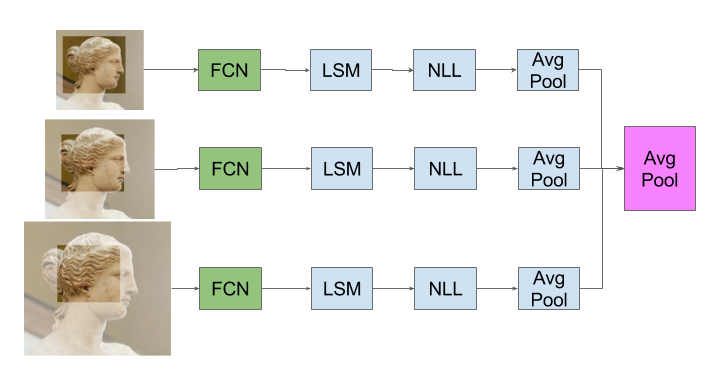
\includegraphics[width=\linewidth]{figures/Average_Loss.png}
    \caption{Calcul de la fonction de coût lorsque l'on entraîne le réseau sur différentes régions à différentes échelles. L'entropie croisée $E$ est calculé pour chaque segment d'image avant d'être moyenné (equation.~\ref{eq:regionloss}).
    \label{fig:regionfinetuning}}
\end{figure}


\section{Apprentissage de régions et de similarité}

Une fois l'apprentissage sur les régions réalisé, nous disposons d'un réseau capable de se focaliser sur une certaine région de l'image.
Nous utilisons ceci pour changer la fonction objectif triple.
Celle définie précédemment (équation~\ref{eq:objectif}) ne prend pas en compte les régions.
Si l'on prend en compte comme région d'intérêt les $k$ éléments avec la plus forte activation du réseau, on peut extraire les caractéristiques depuis uniquement cette zone, qui représente la région la plus probable de présence de l'objet.
Pour la fonction objectif de l'apprentissage, en plus du plongement correct des images positives et négatives, nous ajoutons la classification de cette région avec l'entropie croisée.
Ce qui donne l'équation suivante :

\begin{equation}
\mathcal{L}(x,y,z,\hat{x}) =  \alpha \max(0, x \cdot z - x \cdot y + m) +
(1-\alpha) \frac{1}{k} \sum_{l=1}^k E(x_{h,w}, \hat{x}_{h,w})
\label{eq:proposedloss}
\end{equation}

On retrouve le plongement des images $x,y$ et $z$, qui doivent vérifier l'objectif triple (équation~\ref{eq:objectif}.
Ainsi que la classification des $k$ région de plus forte activation, avec $\alpha$ la régularisation entre les deux objectifs de la fonction de coût.

Dans le but de réaliser cette onction, nous définissons un réseau de neurones entièrement convolutif, capable de produire une sortie de classification de la région de plus grande activation, ainsi qu'un plongement de cette région.
Pour ce faire, une couche de ``pooling'' des $k$ régions de plus forte activation est ajouté à la sortie du réseau. 
En s'inspirant de l'architecture R-MAC~\cite{gordo2016deep}, une normalization $L2$, un décalage et une couche entièrement connectée sont ajoutés à cette sortie.
Ce pipeline permet de réaliser une PCA (Principal Component Analysis) pour réduire la taille de la représentation~\cite{jegou2012negative}.
Les paramètres du décalage sont appris par rétro-propagation et la couche entièrement connecté permet de réduire la taille du descripteur à la taille désirée pour l'espace de projection $\mathbb{E}$.
Une normalisation $L2$ est de nouveau opérée pour normaliser le plongement des images.

\begin{figure}[!htb]
\centering
    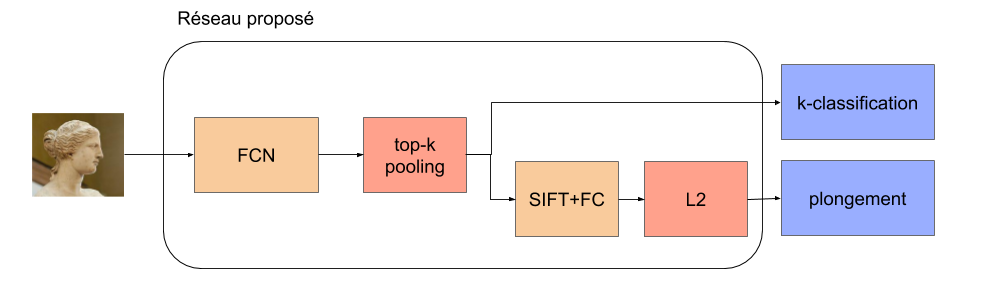
\includegraphics[width=\linewidth]{figures/ProposedNetwork.png}
    \caption{Architecture du réseau proposé basé sur un réseau entièrement connecté pré-entrainé pour détecter les régions d'intérêt.
    \label{fig:proposednetwork}}
\end{figure}

Pour l'entraînement de ce réseau, nous utilisons une architecture à trois branches comme précédemment, à laquelle nous ajoutons la classification des $k$ régions de plus fortes activation, comme montré sur le schéma~\ref{fig:finalpipeline}.
La même stratégie de sélection des triplets que celle utilisée précédemment est appliquée.

%\begin{figure}[!htb]
    %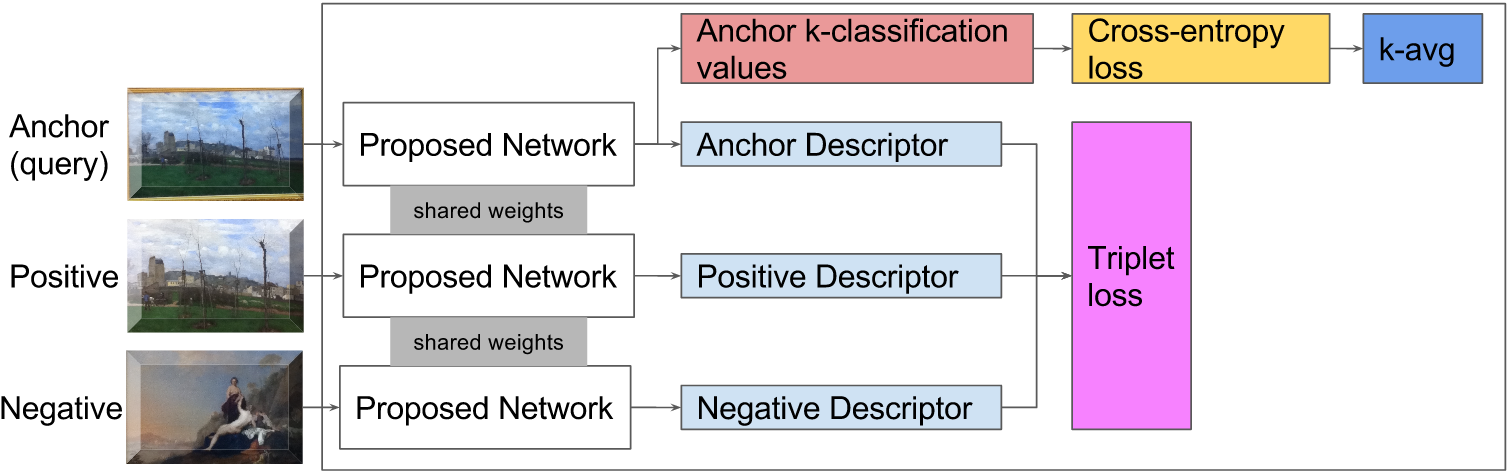
\includegraphics[width=\linewidth]{figures/contrib_train.png}
    %\caption{CORRECT MAIS A REFAIRE CAR NOTATION INCORRECT Proposed architecture for instance search based on an FCN ~\cite{long_fully_2015} for region proposals, at training time
    %\label{fig:contribtrain}}
%\end{figure}

La figure~\ref{fig:finalpipeline} reprend l'ensemble des étapes de l'apprentissage, en incorporant l'apprentissage des régions. 
Les étapes 1 et 2 sont identiques à celles présenté au chapitre précédent.
L'étape 3 correspond à l'apprentissage des régions d'intérêt.
Enfin, l'étape 4 est l'apprentissage grâce à la fonction de coût~\ref{eq:proposedloss}.	
\begin{figure}%
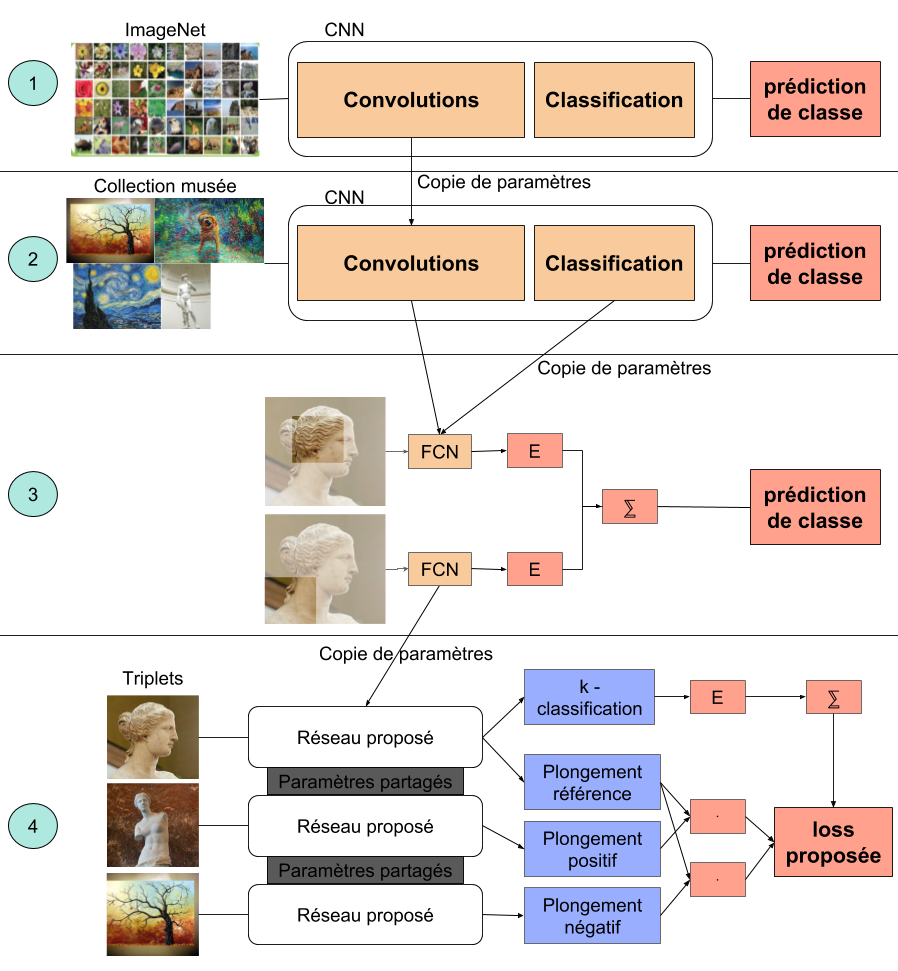
\includegraphics[width=\columnwidth]{figures/pipelinefinal.png}%
\caption{Pipeline final d'apprentissage, avec l'ajout de la détection des régions d'intérêts.}%
\label{fig:finalpipeline}%
\end{figure}


\section{Expérimentation}

Nous testons notre approche sur deux collections du projet GUIMUTEIC, CLICIDE et GaRoFou, et nous évaluons grâce au métriques suivantes :
\begin{itemize}
	\item La précision à 1 (TOP@1) : l'image la plus proche contient le même objet.
	\item La précision moyenne (MAP pour Mean Average Precision) : la moyenne des valeurs de précision des images pertinentes (contenant le même objet) dans la liste ordonnée en fonction des distances.
\end{itemize}






\subsection{Paramètres d'apprentissage}

Pour les premières étapes de l'apprentissage, les mêmes paramètres que dans le chapitre précédent sont utilisés, commes les étapes 1 et 2 sont identiques.
La sélection des triplets se fait également de la même manière que précédemment, à savoir : dans un premier temps tous les triplets négatifs semi-difficiles, puis tous les triplets négatifs difficiles.

Comme nous utilisons un réseau entièrement convolutif, la taille des images pour l'apprentissage est libre, contrairement à un réseau contenant des couches entièrement connectées.
Pour nos expérimentation, nous utilisons une taille fixe pour la plus petit côté des images en entrée, avec deux échelles différentes.
Pour ResNet, nous utilisons deux échelles : $448$ et $224$.
Pour AlexNet, nous avons trouvé que la convergence n'était pas correcte avec les mêmes paramètres, nous utilisons donc les échelles : $384$ et $224$.
Lorsque l'on utilise des images avec des ratio entre hauteur et largeur très grand, l'utilisation de mémoire pendant l'apprentissage peut être très importante. 
Pour limiter cela, nous limitons le ratio au maximum à $2.0$.

Les paramètres de la fonction de coût~\ref{eq:proposedloss} sont $\alpha = 0,5$ et $k=6$.

%The stride of a full network depends on the architecture and is 32
%pixels for the architectures used here: AlexNet and ResNet.
%
%For the processing of the Fully Convolutional networks (step 2 of our proposal, described in part~\ref{sec:contrib}), all images are scaled to have the same number of pixels in the smaller side in order to normalize the sizes of the features present in the images. 
%Note that for large aspect ratios and large scales of the smaller side, the memory consumption of training can be high for single images having a very large aspect ratio.  To limit this spike in memory consumption, the aspect ratios are limited by introducing uniform random noise on the smaller side of images with high aspect ratios. In our experiments, we use a maximal aspect ratio of $2.0$ and images
%at two scales of $448$ and $224$ pixels for the smaller side. We found
%that the AlexNet architecture did not have good convergence behavior,
%thus we used scales of $384$ and $224$ instead.



\subsection{Résultats}
\label{sec:resultatregion}

\begin{table*}
\centering
\begin{tabular}{|l||c|c||c|c|}
\hline & \multicolumn{2}{c||}{\emph{top@1 (en \%)}} &
\multicolumn{2}{c|}{\emph{MAP (en \%)}}\\
\hline & \emph{CLICIDE} & \emph{GaRoFou} & \emph{CLICIDE} & \emph{GaRoFou}\\
\hline \emph{Gordo multi-res~\cite{gordo2016deep}}
& 92.73 & 95.65 & 65.49 & 89.32\\ \hhline{|=||=|=||=|=|}
\hline \emph{AlexNet E} & 72.73 & 85.87 & 32.71 & 66.11\\
\hline \emph{AlexNet Classif} & 78.18 & 90.76 & 38.51 & 72.92\\
\hline \emph{AlexNet SS} & 75.76 & 90.20 & 36.20 & 77.73\\
\hline \emph{AlexNet + Régions} & 81.21 & 83.15 & 45.53 & 71.71\\ 
\hhline{|=||=|=||=|=|}
\hline \emph{ResNet E} & 72.12 & 85.33 & 40.99 & 70.15\\
\hline \emph{ResNet Classif} & 79.39 & 94.57 & 75.11 & \textbf{93.44}\\
\hline \emph{ResNet SS} & 85.45 & 95.11 & \textbf{83.00} & 91.90\\
\hline \emph{ResNet + Régions} & \textbf{94.55} & \textbf{96.20}
& 82.94 & 91.83\\
\hline
\end{tabular}
\caption{TOP@1 et MAP des différentes approches sur les collections CLICIDE et GaRoFou.
\label{tab:results}}
\end{table*}



Le tableau~\ref{tab:results} présente les résultats obtenu sur CLICIDE et GaRoFou par l'approche proposée, comparé aux approches précédentes.
Nous remarquons que notre méthode obtient le meilleur TOP@1, avec un score de 94.55\% comparé aux 92.73\% de l’état de l’art sur CLICIDE.
Sur GaRoFou, les méthodes de l’état de l’art obtiennent un score de 95.65\%, le gain est moins important, avec 0.55\%.
Comme montré précédemment, ResNet présente toujours de meilleurs résultats que AlexNet.
L'apport de la propositions de régions par le réseau, même sans base d'apprentissage annotées, permet donc d'améliorer les résultats.
Toutefois, si l'on s'intéresse à la MAP, on voit qu'aucune des méthodes proposées ne permet d'obtenir de meilleurs résultats qu'un réseau Siamois Simple (SS), où qu'un fine-tuning dans le cas de GaRoFou (Classif).
Cela nous amène à penser que même si le TOP@1 est bon, l'espace de projection créé ne capture pas complètement la similarité entre les images.



\section{Indexation et augmentation de données côté base de données}

Pour l'identification d’instance, nous utilisons la recherche du plus proche voisin dans la base de données d’image.
Un parcours simple de cette base de donnée est suffisant, étant donné la taille de nos collection.
On peut même augmenter le nombre d’éléments dans la base de données, ce qui est nommé ``Database-side feature augmentation''~\cite{turcot_better_2009,arandjelovic_three_2012}.
Cela permet d’améliorer la recherche, en couvrant plus l’espace de recherche.

Pour modifier les éléments dans l’espace de projection, il y a deux stratégies : soit ajouter des points dans l'espace, soit de changer le plongement de chaque élément de la base de données.
On peut par exemple remplacer chaque éléments de l'espace par une combinaison de ces $k$ plus proches voisins, ce qui permet de lisser les projections, et de corriger le bruit~\cite{gordo2016deep}. 
Dans notre cas, nous disposons généralement de peu d'image références pour chaque objet, nous n'envisageons donc pas de modifier les plongement en fonction de leur voisin, mais plutôt de créer de nouvelles projections, pour rendre l'espace plus dense.

Pour l’ensemble des exemples d’une instance, nous prenons chacun des plongements, et calculons leur moyenne.
Ce nouveau vecteur peut être considéré comme un nouvel exemple pour l'instance donnée.
Nous pouvons donc l'ajouter à l'espace de projection.
Ce nouveau point peut également servir de référence pour l’instance qu’il représente, ce qui permet de supprimer tous les autres éléments de l’espace.
Ainsi, le nombre d'éléments à parcourir pour la recherche du plus proche voisin n’est plus l’ensemble des exemple, mais uniquement un pour chaque instance.


 %proposes to combine descriptors of the reference images in order to form better database-side descriptors.
%Every reference descriptor is simply replaced by a combination of itself and the $k$ nearest neighbors. 
%This combination is computed as a weighted sum, weighted by the rank of the neighbors with respect to $k$ (the closest neighbor has the highest weight and the $k$-th neighbor the lowest).
%
%In our work, we use a technique called Instance Feature Augmentation.
%We use the fact that we know the corresponding label for each image in our dataset.
%For each label, we compute the representation of an instance by averaging the features of every images corresponding to this label. 
%This representation is added to the dataset as a new instance.
%We show that this approach does not improve mean precision@1, but gives a better Mean Average Precision. 
%This suggests that the internal representation of the instance is improved. 

Le tableau~\ref{tab:resultsAugmentation} montre les résultats obtenu avec l'augmentation de données de la base de donnée par rapport au résultats précédents.
L'ajout de l'augmentation de donnée n'améliore pas le top@1, voir même la détériore, avec en moyenne une perte de 0.5\%.
Par contre, on remarque une nette amélioration de la MAP, ce qui signifie que les nouveaux exemples créé dans la base de donnée capture bien certaines instances.

\begin{table*}
\centering
\begin{tabular}{|l||c|c||c|c|}
\hline & \multicolumn{2}{c||}{\emph{TOP@1 (en \%)}} &
\multicolumn{2}{c|}{\emph{MAP (en \%)}}\\
\hline & \emph{CLICIDE} & \emph{GaRoFou} & \emph{CLICIDE} & \emph{GaRoFou}\\
\hline \emph{AlexNet proposé} & 81.21 & 83.15 & 45.53 & 71.71\\
\hline \emph{AlexNet proposé + Augmentation} & 80.61 & 82.61 & 71.02 & 81.66\\ 
\hhline{|=||=|=||=|=|}
\hline \emph{ResNet proposé} & \textbf{94.55} & \textbf{96.20}
& 82.94 & 91.83\\
\hline \emph{ResNet proposé + Augmentation} & 93.94 & 95.11
& \textbf{94.23} & \textbf{93.86}\\
\hline
\end{tabular}
\caption{TOP@1 et MAP sur les corpus CLICIDE et GaRoFou, avec et sans l'augmentation de données coté base de données.}
\label{tab:resultsAugmentation}
\end{table*}


\begin{figure}
  \centering
  \begin{minipage}[c]{.33\linewidth}
    \centering
    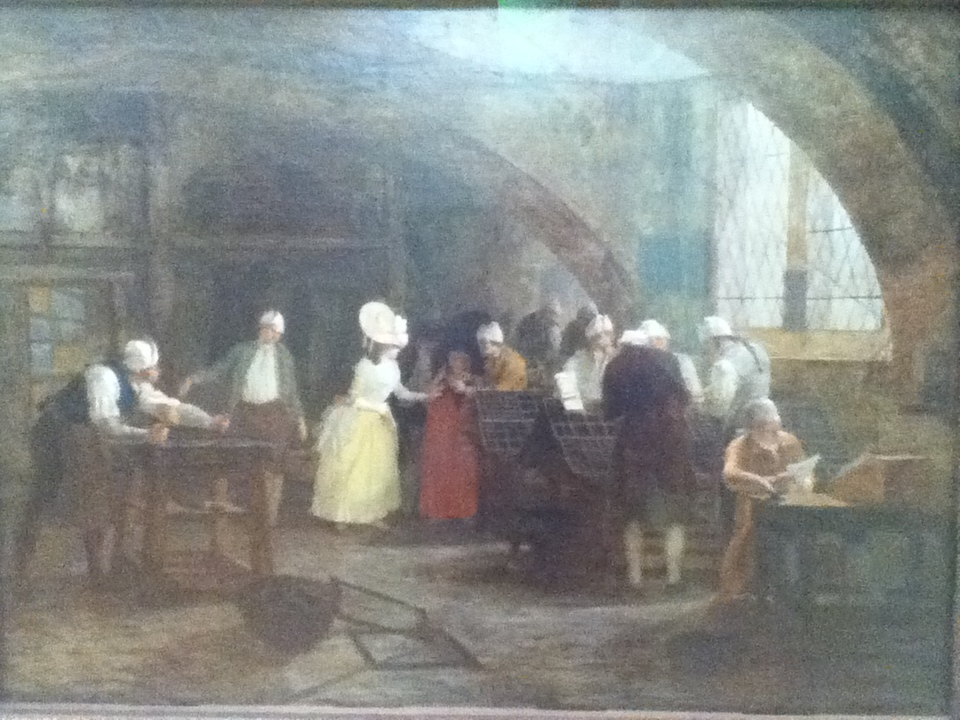
\includegraphics[width=\textwidth]{figures/11J-0521.JPG}
  \end{minipage} \hfill
  \begin{minipage}[c]{.33\linewidth}
    \centering
    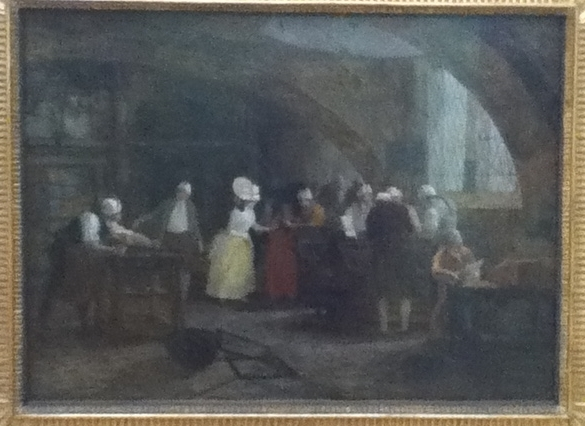
\includegraphics[width=\textwidth]{figures/11J-1.JPG}
  \end{minipage}
  \begin{minipage}[c]{.32\linewidth}
    \centering
    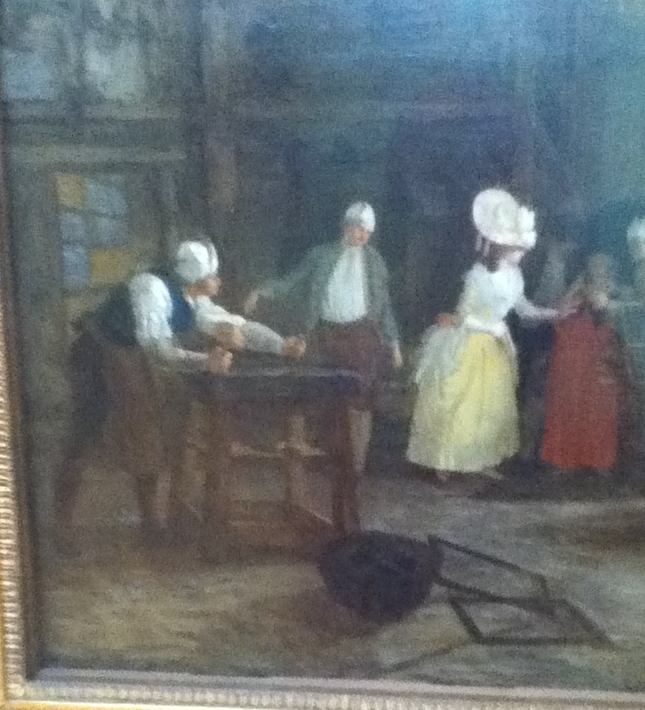
\includegraphics[width=\textwidth]{figures/11J-4.JPG}
    %\caption{Heat-map for 10A\label{fig:sample1_hm}}
  \end{minipage}

  \begin{minipage}[c]{.33\linewidth}
    \centering
    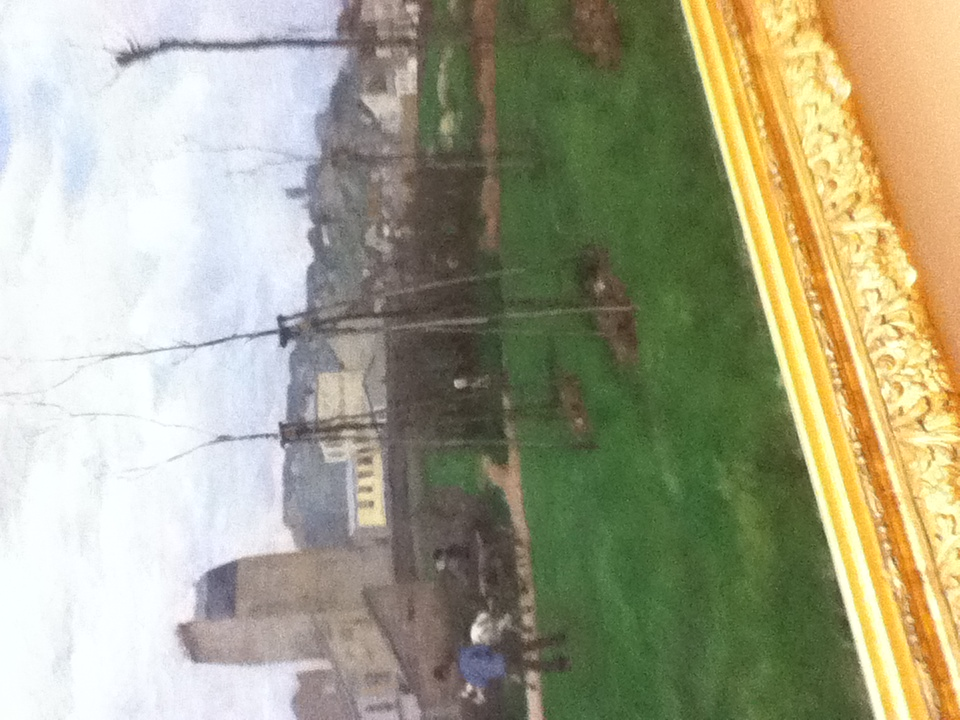
\includegraphics[width=\textwidth, angle=270]{figures/23D-0740.JPG}
  \end{minipage} \hfill
  \begin{minipage}[c]{.33\linewidth}
    \centering
    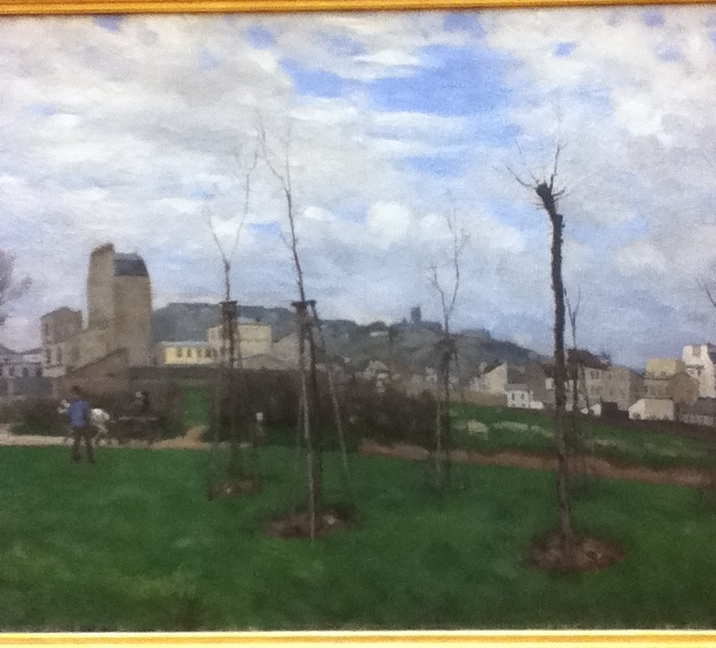
\includegraphics[width=\textwidth]{figures/23D-2.JPG}
  \end{minipage}
  \begin{minipage}[c]{.32\linewidth}
  	\centering
    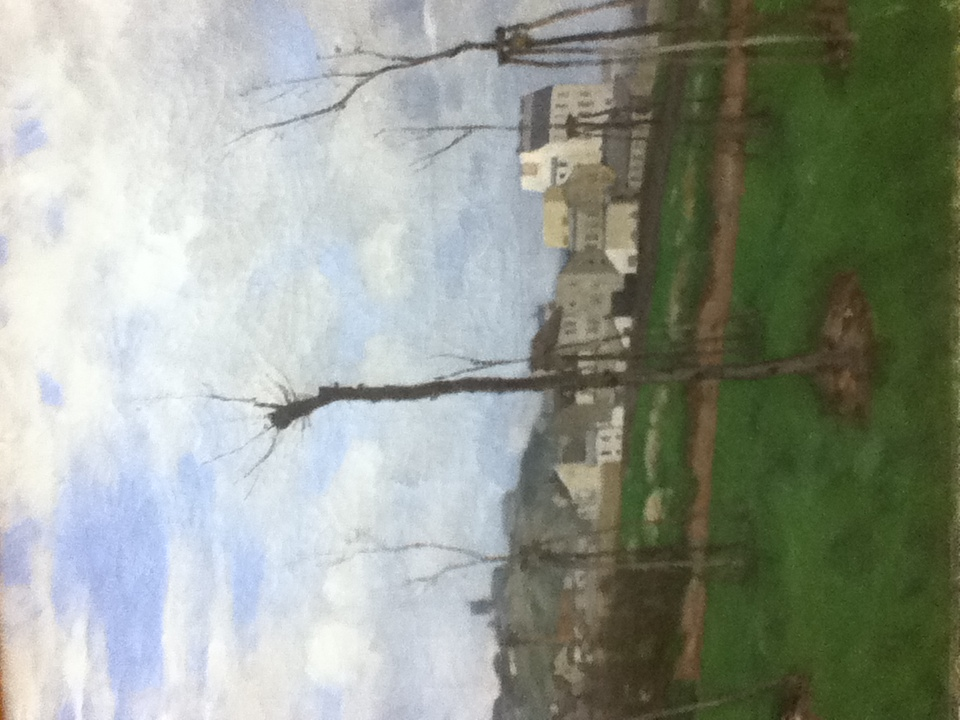
\includegraphics[width=\textwidth, angle=270]{figures/23D-1.JPG}
    %\caption{Heat-map for 10A\label{fig:sample1_hm}}
  \end{minipage}
  
  \begin{minipage}[c]{.33\linewidth}
    \centering
    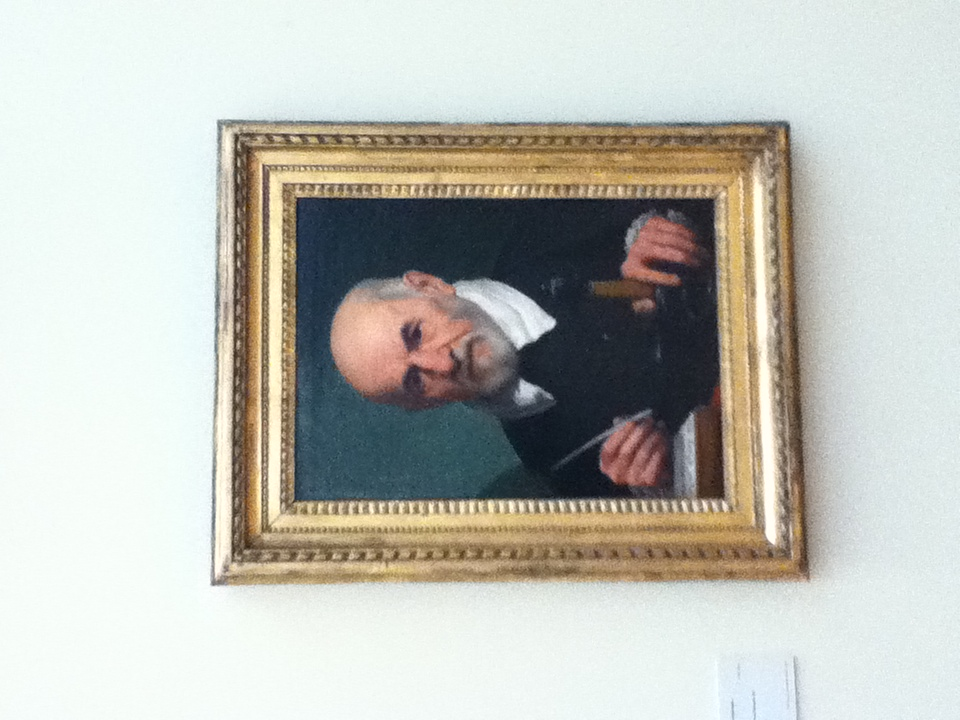
\includegraphics[width=\textwidth, angle=270]{figures/1C-0454.JPG}
  \end{minipage} \hfill
  \begin{minipage}[c]{.33\linewidth}
    \centering
    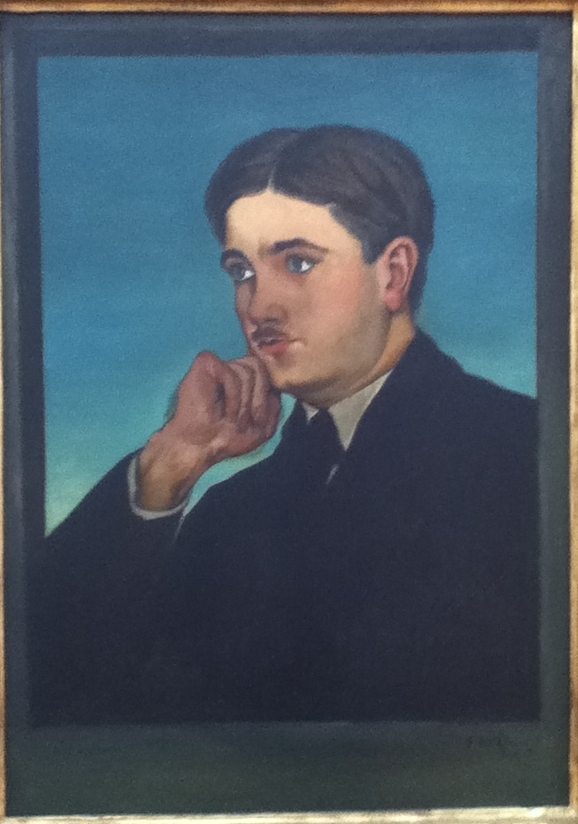
\includegraphics[width=\textwidth]{figures/1.png}
  \end{minipage}
  \begin{minipage}[c]{.32\linewidth}
    \centering
    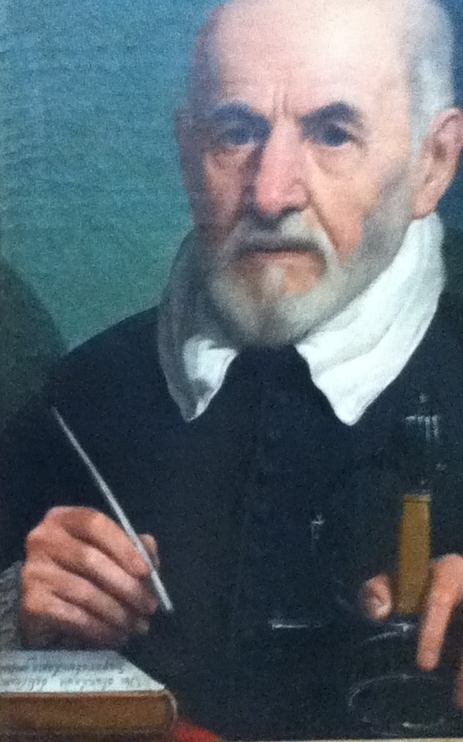
\includegraphics[width=\textwidth]{figures/1C-0.JPG}
    %\caption{Heat-map for 10A\label{fig:sample1_hm}}
  \end{minipage}
  
  
  \begin{minipage}[c]{.33\linewidth}
    \centering
    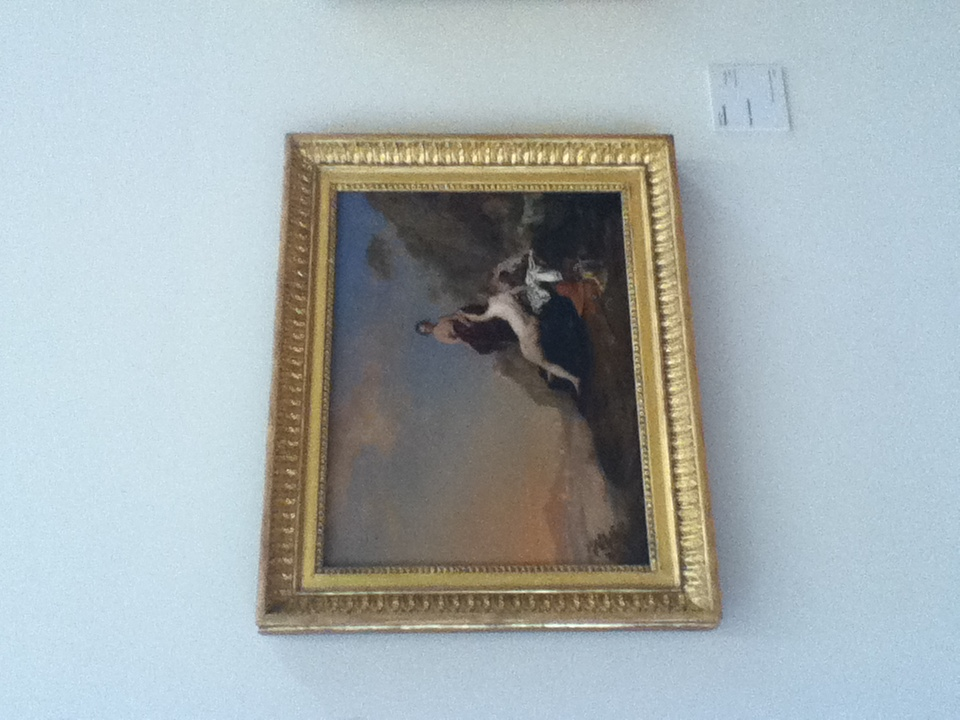
\includegraphics[width=\textwidth, angle=270]{figures/5B-0506.JPG}
  \end{minipage} \hfill
  \begin{minipage}[c]{.33\linewidth}
    \centering
    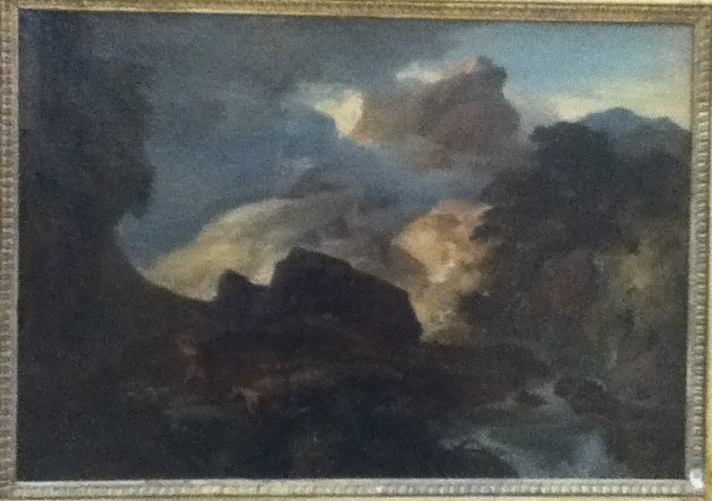
\includegraphics[width=\textwidth]{figures/2.png}
  \end{minipage}
  \begin{minipage}[c]{.32\linewidth}
    \centering
    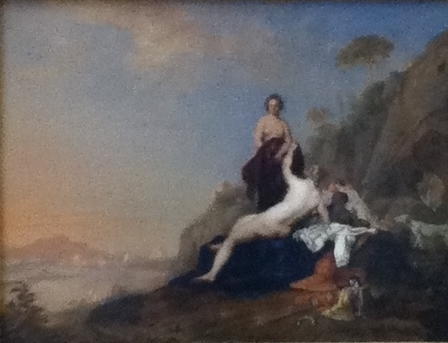
\includegraphics[width=\textwidth]{figures/5B-0.JPG}
    %\caption{Heat-map for 10A\label{fig:sample1_hm}}
  \end{minipage}
  
\caption{Exemples de succès et d'échecs de notre approche. La première colonne représente les requêtes, les deuxième colonne contient les images les plus proches et la troisième colonne la deuxième image la plus proche dans la collection CLICIDE.}
\label{fig:failing}
\end{figure}

La figure~\ref{fig:failing} montre quelques exemples de succès et d'échecs de notre approche.
Pour chaque requêtes (colonne de gauche), on affiche les deux images les plus proches.
On remarque que dans les échecs, la deuxième image retournée est la bonne (la TOP@2 est de 100\%).
L'augmentation de données dans l'espace de projection permet donc de créer un espace plus dense, qui capture mieux la similarité entre les images.
Même si cela n'améliore pas la TOP@1 dans notre cas, cela permet d'envisager d'autre approches pour la détection d'instance, notamment si l'on s'intéresse aux vidéos, avec par exemple un vote majoritaire ou une moyenne des instances retournées.

Notre approche permet donc d'obtenir de meilleurs résultats que les méthodes de l'état de l'art, dans le cas des corpus de petites tailles.
Notre solution d'apprentissage de régions non supervisé permet d'avoir une proposition de régions d'intérêts par le réseau.
La proposition de régions pour la création du plongement semble être un point clef pour la recherche d'instance dans les images.
Enfin, une densification de l'espace de projection par augmentation de données permet de mieux capturer la similarité entre les images dans l'espace de projection, avec cependant une perte en précision.





\chapter{Détection de gestes}
\label{chap:gestes}

Nous avons proposé, dans le chapitre précédent, une nouvelle approche pour l'identification d'instance sur les images.
Nous nous intéressons dans ce chapitre à l'interaction avec l'utilisateur, à travers ses gestes.
L'étude participatives détaillée dans le chapitre~\ref{chap:etude} intitulé ``\nameref{chap:etude}’’, en annexe~\ref{sec:etudeGestes}, a mis en évidence 5 gestes utiles pour l'interaction entre l'utilisateur et le système GUIMUTEIC.
L'objectif de ce chapitre est de présenter une solution pour la détection de gestes dans le cadre du projet, basé sur la caméra embarquée.

Nous avons pour contrainte de faire fonctionner cette détection de geste sur appareil mobile, en continu, pour être capable de réagir aux actions de l'utilisateur.
L'objectif est double : avoir une bonne reconnaissance des gestes, avec un minimum de calculs pour être capable de fonctionner sur processeur mobile.
Nous nous intéressons dans un premier temps aux réseaux de petites tailles et aux temps de calculs faible, pour proposer un réseau de neurones profond performant et compact (section~\ref{sec:reseausimple}).
Nous étendons ensuite cette nouvelle architecture pour qu'elle soit capable de regarder plusieurs trames de la vidéos.
En ajoutant une fusion de l'information venant de plusieurs trames, nous obtenons une solution efficace, ayant les mêmes performances que les architectures de l'état de l'art, avec considérablement moins de paramètres (section~\ref{sec:multiframe}).
Nous évaluons nos propositions sur un corpus de vidéos de gestes conçu dans le cadre du projet GUIMUTEIC, présenté en détail en annexe~\ref{sec:corpusGestes}.


%%%%%%%%%%%%%%%%%%%%%%%%%%%%%%%%%%%%%%%%%%%%%%%%%%%%%%%%%%%%%%%%%%%%%%%%%%%%%%%%%%%%%%%%%%%%%%%%%%%%
%
%			Single Frame
%
%
%%%%%%%%%%%%%%%%%%%%%%%%%%%%%%%%%%%%%%%%%%%%%%%%%%%%%%%%%%%%%%%%%%%%%%%%%%%%%%%%%%%%%%%%%%%%%%%%%%%%
\section{Utilisation des convolutions groupées pour réduire la complexité}
\label{sec:reseausimple}

Notre objectif est de proposer une architecture de réseau qui soit à la fois assez compacte et rapide pour être utilisable sur processeur mobile, et suffisamment performante pour être au niveau de l'état de l'art. 
Nous avons présenté dans la section~\ref{sec:petitsreseaux}, un état de l'art des réseaux de petites tailles, et nous nous basons sur ceux-ci pour créer notre architecture.
Les réseaux de petites tailles tels que MobileNet~\cite{howard2017mobilenets}, SqueezeNet~\cite{iandola2016squeezenet} ou ShuffleNet~\cite{zhang2017shufflenet} utilisent les principes présentés par Simonyan et Zisserman~\cite{simonyan2014very}.
Le premier étant de n'utiliser que des convolutions $3*3$, ou équivalents.
Ce type de convolutions étant coûteux en paramètres et en temps de calcul, nous proposons de les remplacer par deux convolutions avec moins de paramètres (section~\ref{sec:remplacer}).
Le deuxième principe à respecter est d'utiliser deux types de convolutions en alternance : un premier ne modifions pas le taille des entrées et un deuxième qui diminue la taille des entrées, mais augmente le nombre de canaux.
En enchaînant ces deux types de blocs, on peut construire des réseaux très profonds, tout en conservant le plus d'informations le long du réseau.
Nous proposons deux nouveaux blocs S1 (section~\ref{sec:S1}) et S2 (section~\ref{sec:S2}) qui correspondent à ces critères avec un nombre de paramètres réduits.



\subsection{Remplacer les convolutions $3*3$}
\label{sec:remplacer}

Les convolutions $3*3$ sont, depuis VGG~\cite{simonyan2014very}, quasiment les seules convolutions utilisées dans les réseaux de neurones.
En en combinant plusieurs, il est possible de réaliser des convolutions de n'importe quelle taille, avec l'avantage de pouvoir mettre entre chaque convolution une opération non linéaire (neurones ReLU) ou des opérations de régularisation (\textit{Batch-Norm}), qui améliorent la convergence de réseau et sa généralisation.
Cependant, dans le cas des réseaux compacts, les convolutions représentent jusqu'à 89\% du total des calculs fait par le réseau~\cite{ma2018shufflenet}.

Pour remplacer les convolutions $3*3$, nous utilisons une combinaison d'une convolution $3*3$ \textit{DeepWise}, présentée dans la section~\ref{sec:groupedConv}, et une convolution $1*1$.
La convolution $3*3$ \textit{DeepWise} (DW-Conv3x3) est une convolution où chaque canal de sortie n'est connecté qu'à un seul canal d'entrée.
La convolution $1*1$ ne s'intéresse qu'à un pixel, sur chacun des canaux.
On obtient ainsi une information au niveau du voisinage du pixel avec la première convolution, et une fusion des informations des différents canaux grâce à la deuxième.
En combinant les deux comme sur la figure~\ref{fig:conv31}, nous obtenons une opération proche d'une convolution $3*3$ au niveau des performances~\cite{howard2017mobilenets}, avec moins de paramètres.


\begin{figure}%
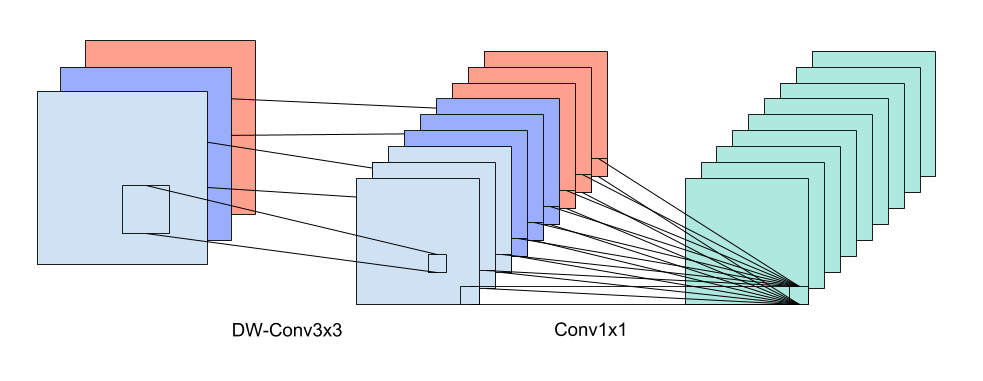
\includegraphics[width=\columnwidth]{figures/groupConvolutionPlusFusion.png}%
\caption{Convolution $3*3$ DeepWise suivie d'une convolution $1*1$ qui fait office de fusion.}%
\label{fig:conv31}%
\end{figure}

Au niveau de la complexité, une convolution $3*3$ sur 32 canaux d'entrée, avec 32 canaux de sortie, contient $ (3*3)*32*32 + 32 = 9248$ paramètres.
Une convolution $3*3$ DeepWise contient pour sa part uniquement $ (3*3)*32 + 32 = 320$ paramètres, comme on supprime toutes les connexions entre les canaux, soit 32 fois moins de connexion.
La convolution $1*1$ toujours avec 32 canaux contient $(1*1)*32*32 + 32 = 1056$ paramètres.
On obtient donc au final en combinant les deux $ 320 + 1056 = 1376$ paramètres, ce qui représente une diminution de 85\% par rapport au 9248 de la convolution $3*3$.


Nous comparons dans le tableau~\ref{tab:convG} les temps de calcul des différentes couches sur un processeur Quad Core cadencé à 2.60GHz, sous Linux 64 bits\footnote{Tous les calculs présentés dans la suite sont réalisés sur la même machine}, en utilisant le framework Pytorch\footnote{\url{https://pytorch.org}}. 
On observe une diminution passant de 23.9 millisecondes pour la convolution $3*3$ à 13.1 millisecondes pour la combinaison de la convolution $3*3$ DeepWise et de la convolution $1*1$, soit une diminution de 45\%. 
Nous utilisons les temps sur CPU, et non pas sur GPU, car nous nous intéressons au déploiement de notre réseau, et non pas à son entrainement, qui lui est réalisé sur GPU.
Pour obtenir des écarts stables et significatifs entre les différents runs, nous utilisons des batchs de 64 images, chacune d'une taille de $32*32$.

\begin{table}[!htb]
\centering
\begin{tabular}{|l|c|c|}
\hline
couche & \# paramètres & temps de calcul (ms) \\
\hline
\hline
Conv3x3 & 9248 & 23.9 \\
\hline
Conv3x3G & 320 & 9.94\\
\hline
Conv1x1 & 1056 & 4.06\\
\hline
Conv3x3G + Conv1x1 & 1376 & 13.1~\footnote{A noter que le temps de calcul de la convolution $3*3$ groupée suivie de la convolution $1*1$ n'est pas égal à la somme arithmétique des temps de calcul de chacune de ces opérations prises séparément. Cela vient de l'optimisation faite par le Framework utilisé (Ici Pytorch) dans l'enchaînement des opérations.} \\
\hline
\end{tabular}
\caption{Tableau de comparaison du nombres de paramètres et du temps de calculs des convolutions groupées et non groupées}
\label{tab:convG}
\end{table}

Nous avons donc un moyen de remplacer les convolutions $3*3$ pour minimiser le nombre de paramètres, et donc l'occupation mémoire, et les temps de calculs.
Cependant, nous souhaitons également tirer avantages des \textit{skip-connection} et de la régularisation.
Nous présentons dans la suite deux nouveaux types de blocs, remplaçant les convolutions $3*3$ par ce que nous avons présenté, et ajoutant des connexions et de la régularisation.


\subsection{Bloc S1}
\label{sec:S1}


Nous avons énoncé précédemment (section~\ref{sec:cnn}) l'utilité d'avoir deux types de blocs de convolutions, avec l’un qui conserve la taille des entrées que nous nommons S1, et l’autre qui divise par deux la taille des entrées, en multipliant le nombre de canaux, nommé S2.
Le bloc S1 que nous proposons est composé de la combinaison des convolutions présentées précédemment.
Tout d'abord une convolution $3*3$ DeepWise, avec un pas de 1 et un remplissage (padding) de 1, pour conserver la taille des entrées.
Ensuite, une convolution $1*1$ avec pas de 1 et pas de remplissage, chargée de faire la fusion des informations des différents canaux.
Pour améliorer la généralisation de notre réseau, nous ajoutons après chacune de ces couches, une \textit{batch-normalisation}.
Nous utilisons également le fait d'avoir remplacé la convolution $3*3$ par deux convolutions pour mettre une couche de neurones ReLU entre les deux, ce qui augmente la non-linéarité du bloc. 
Nous proposons également une \textit{skip-connection} entre l'entrée et la sortie du bloc, pour permettre une meilleur propagation du gradient~\cite{he2015delving}.
La figure~\ref{fig:S1} montre une représentation graphique du bloc S1, et le code qui réalise cette fonction est indiqué en annexe~\ref{sec:implementationS1}.


\begin{table}[!htb]
\centering
\begin{tabular}{|c|c|}
\hline
\#couche & type de couche \\
\hline
\hline
1 & convolution $3*3$ DeepWise, pas de 1, remplissage de 1 \\
\hline
2 & \textit{batch-normalisation}\\
\hline
3 & neurones ReLU\\
\hline
4 & convolution $1*1$, pas de 1, pas de remplissage\\
\hline
5 & \textit{batch-normalisation}\\
\hline
6 & neurones ReLU \\
\hline
7 & fusion des informations entre l'entrée et la sortie par addition\\
\hline

\end{tabular}
\caption{Composition du bloc S1.}
\label{tab:S1}
\end{table}



\begin{figure}%
\centering
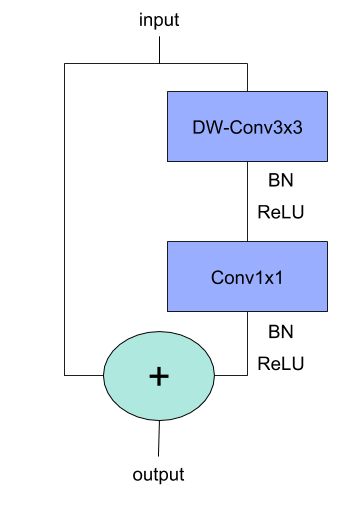
\includegraphics[width=.45\columnwidth]{figures/stride1.png}%
\caption{Schéma du module S1.}%
\label{fig:S1}%
\end{figure}

Les temps de calculs, rapportés dans le tableau~\ref{tab:blocS1}, montrent une large augmentation du temps de calcul, due à l'ajout de la \textit{batch-normalisation} et des couches ReLU.
Si on compare au tableau précédent, on passe de 13.1ms à 23.9ms.
Cependant, au niveau des paramètres, on ajoute ici uniquement ceux de la \textit{batch-normalisation}, ce qui donne un total 1504. 
Nous comparons notre bloc aux blocs ``Fires'' de SqueezeNet~\cite{iandola2016squeezenet} et ``Shuffle'' proposé par ShuffleNet~\cite{zhang2017shufflenet} dans le tableau~\ref{tab:blocS1}.
Ces deux blocs se basent sur la diminution du nombre de canaux entre les deux couches de convolutions, pour réduire le nombre de canaux d'entrée pour la convolution $3*3$, ce qui permet de réduire le nombre de paramètres.
Les deux réseaux doivent utiliser une coûteuse convolution $3*3$ en première couche pour extraires les premières informations de l'image.
Comme le bloc S1 a pour but de pouvoir remplacer toutes les convolutions, nous pouvons nous passer de cette couche, ce qui réduit le nombre de paramètres du réseau final.
On voit dans la tableau que le bloc S1 est plus lent, 23.9ms, que les bloc Fire (22.3ms) et Shuffle (21.8ms).
 

\begin{table}[h]
\centering
\begin{tabular}{|l|c|c|}
\hline
Bloc & \# paramètres & temps de calcul (ms) \\
\hline
\hline
Conv3x3DW + Conv1x1 & 1376 & 13.1 \\
\hline
Fire Bloc & 2888 & 22.3 \\
\hline
Shuffle Bloc & 472 & 21.8 \\
\hline
Bloc S1 & \textbf{1504} & \textbf{23.9}\\
\hline
\end{tabular}
\caption{Tableau de comparaison des blocs des réseaux de tailles réduites avec le bloc S1}
\label{tab:blocS1}
\end{table}

Notre bloc S1 permet donc de remplacer une convolution $3*3$, avec un nombre de paramètres inférieur et en ajoutant une \textit{skip-connection}.
Il est fait pour conserver la taille des tailles des entrées, en ne modifiants ni les tailles des filtres, ni le nombre de canaux.
Nous définissons dans la partie suivante le bloc S2, qui peut agir sur le nombre de canaux, et qui va diviser par deux la tailles des filtres d'entrée.


\subsection{Bloc S2}
\label{sec:S2}

Pour remplacer les convolutions qui réduisent la taille des entrées, et notamment la première couche $3*3$ utilisée par la plupart des résaux, nous définissons le bloc S2
Nous voulons toujours prendre avantage des \textit{skip-connection}, mais cette fois-ci nous avons une diminution de la taille de l'entrée et un changement du nombre de canaux, il n'est donc pas possible de directement additionner l'entrée et la sortie.
Tout d'abord le nombre de canaux étant différent, nous proposons de remplacer l'addition par une concaténation.
Ceci permet de garder les apports des \textit{skip-connection}, avec des résultats proches de ceux de l'addition~\cite{he2015delving, zhang2017shufflenet, ma2018shufflenet}.
Cependant, pour pouvoir réaliser la concaténation, chaque canal doit avoir la même taille.
Nous proposons donc de fixer le changement de taille à une division par deux de la taille.
Ainsi, inspiré par~\cite{ma2018shufflenet}, en appliquant un \textit{Average-Pooling} de $3*3$, avec un pas de 2 et un remplissage de 1, on obtient une sortie deux fois plus petite, qu'il est possible de concaténer à la sortie des couches de convolutions.

La partie convolution de ce bloc est très proche de celle du bloc S1, avec uniquement un changement de la première couche.
La couche de convolution $3*3$ DeepWise est appliquée avec un décalage de 2 et un remplissage de 2, ce qui a pour effet de diminuer la taille des entrées par deux.
Le nombre de canal de sortie du bloc est défini comme le double du nombre de canal d'entrée.
La bloc S2 (figure~\ref{fig:S2} représente la bloc S2, avec sur la partie gauche l'opération de Pooling pour diminuer la taille des entrées, et sur la droite, les couches de convolutions.

\begin{figure}%
\centering
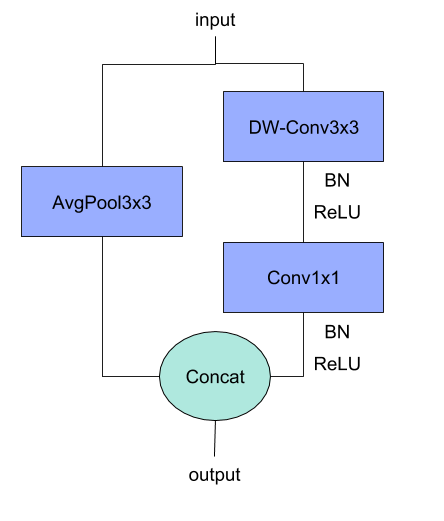
\includegraphics[width=.6\columnwidth]{figures/stride2.png}%
\caption{Schéma du module S2.}%
\label{fig:S2}%
\end{figure}


Le nombre de paramètres, observé dans la deuxième colonne du tableau~\ref{tab:blocS2}, ne change pas par rapport au bloc S1.
Nous pouvons le comparer au bloc Shuffle avec décalage de 2, qui utilise la concaténation aussi pour faire la fusion entre entrées et sorties.
Ce bloc à 848 paramètres, mais un temps d'exécution de 14.9ms, comparé à 13.2ms pour le bloc S2. 
Le bloc S2 est beaucoup plus rapide que le bloc S1, venant du fait qu'il applique deux fois moins les convolutions $3*3$, étant donné qu'il utilise un décalage de 1.

\begin{table}[h]
\centering
\begin{tabular}{|l|c|c|}
\hline
Bloc & \# paramètres & temps de calcul (ms) \\
\hline
\hline
Shuffle Bloc Stride 2 & 848 & 14.9 \\
\hline
Bloc S2 & \textbf{1504} & \textbf{13.2}\\
\hline
\end{tabular}
\caption{Tableau de comparaison des blocs ``Shuffle Stide 2'' et S2}
\label{tab:blocS2}
\end{table}



\subsection{Réseau de classification de gestes à base de S1 et S2}

Dans cette partie, nous construisons un réseau profond en utilisant les blocs S1 et S2.
Avec pour objectif d’obtenir un réseau avec un nombre de paramètres faible, et une vitesse d'exécution réduite par rapport aux réseau profonds de grandes taille, comme AlexNet ou ResNet, mais également plus petit que SqueezeNet ou ShuffleNet.
Inspiré par les micro-architectures récentes~\cite{howard2017mobilenets, zhang2017shufflenet,hu2017squeeze, iandola2016squeezenet} et également par VGG~\cite{simonyan2014very}, nous proposons de remplacer toutes les convolutions $3*3$ par des blocs S1, et toutes les convolution $3*3$ avec décalage de 2, qui font donc du sous échantillonnage, par le bloc S2. 

Comme montré sur la figure~\ref{fig:reseau1frame}, en partant d'une image $224*224*3$, on applique successivement les blocs S1 (sans réduire la taille) et S2 (en réduisant et en augmentant le nombre de canaux, jusqu'à obtenir une dimension suffisante pour la classification, ici $7*7*1024$.
Un \textit{Average-Pooling} de $7*7$ est alors appliqué, pour obtenir une matrice de $1*1*1024$.
Une couche entièrement connectée est alors utilisé pour réduire la dimension de 1024 à 6, notre nombre de gestes à reconnaître.

\begin{figure}
\centering
\includegraphics[width=\columnwidth]{figures/Reseau1frame.pdf}%
\caption{Schéma du réseau proposé pour la reconnaissance de geste, avec entre chaque connection la taille de la matrice de représentation des données.}%
\label{fig:reseau1frame}%
\end{figure}


Nous comparons notre réseau en terme de taille à des réseaux de petites tailles, tels que SqueezeNet, MobileNet et ShuffleNet, ainsi qu’à des réseaux comme AlexNet et ResNet pour donner une idée des ordres de grandeur.
Les résultats de cette comparaison sont présentés dans le tableau~\ref{tab:networkscomparison}.
Pour comparer ces réseaux entre eux, nous nous basons sur le même framework, c'est pourquoi les résultats peuvent différer de ceux présentés dans les publications originales respectives.
Les expérimentations sont réalisées avec des batch de 8 images de taille 224x224 à trois canaux.

Nous voyons que notre modèle est celui qui propose le moins de paramètres avec 772 millions de paramètres contre 922 millions, sans être pour autant le plus rapide 0.284 secondes contre 0.226 pour ShuffleNet.
Cela venant du fait que nous utilisons plus d'\textit{average-pooling} et de \textit{batch-normalisation} que les autres modèles.
L'objectif de notre réseau est de fournir une occupation mémoire la plus faible possible, pour pouvoir être utilisé sur mobile, à côté de notre réseau de reconnaissance d'instance (section~\ref{chap:regions}).
En terme de temps de calcul, il est de l'ordre de grandeur des réseau spécialisés pour les applications mobiles que sont MobileNet, SqueezeNet et ShuffleNet.

Nous n'avons donc pas de problème niveau temps d'exécution, et préférons optimiser l'utilisation de la mémoire, qui est dans notre cas plus problématique, dans le sens où elle doit être partagée avec le réseau de reconnaissance d'œuvres.

\begin{table}
\centering
\begin{tabular}{|l|c|c|}
\hline
\hline
Modèle & \# paramètres (en millions) & Temps de calcul (secondes) \\
\hline
SqueezeNet & 1.235 & 0.268 \\
\hline
MobileNet & 4.231 & 0.631~\footnote{Bien qu'ayant le nombre de paramètres et les mêmes couches que dans leur papier~\cite{howard2017mobilenets}, nous obtenons un réseau particulièrement lent, avec un réseau qui est normalement presque 40\% plus rapide que AlexNet. Nous mettons cela sur le compte de notre implémentation.} \\
\hline
ShuffleNet & 0.922 & \textbf{0.226} \\
\hline
Notre modèle & \textbf{0.772} & 0.284 \\
\hline
\hline
AlexNet & 61.100 & 0.380 \\
\hline
ResNet & 60.192 & 4.69 \\
\hline
\end{tabular}
\caption{Comparaison des réseaux de neurones, de petite et de grande taille.}
\label{tab:networkscomparison}
\end{table}

Notre réseau, qui nous nommons par la suite le modèle SimpleTrame, est un réseau de petite taille, adapté au processeur mobile, avec un temps d'exécution proche des micro-architecture de l'état de l'art.
Dans la partie suivante, nous nous intéressons aux performances de notre architecture dans la tâche de reconnaissance de geste dans les vidéos à la première personne.

\subsection{Evaluation}

Nous comparons notre réseau SimpleTrame avec les différentes réseaux de l'état de l'art présenté précédemment, sur la tâche de reconnaissance de geste.
Le corpus utilisé est présenté en annexe~\ref{sec:corpusGestes}. 
Il s'agit d'une collection de vidéo à la première personne, contenant les 6 gestes du projet GUIMUTEIC (5 geste + absence de geste).
Il est composé de 29 heures de vidéos, représentant 1669 séquences avec un geste et 1830 séquences sans gestes, ce qui fait un total de 120 000 images.
Ce corpus est séparé en trois groupes, 80\% de séquences d'entraînement, 10\% de séquence de validation et 10\% pour le test.
Les résultats rapportés dans le tableau~\ref{tab:singleframe} représentent la précision sur la partie test de cette collection.
Pour que la classification d'une séquence soit correcte, il faut que la majorité des images de la séquence soient classifiées correctement par le réseau.

\begin{table}
\centering
\begin{tabular}{|l|c|c|}
\hline
Modèle & \#paramètres (en million) & Précision (en pourcent) \\
\hline
\hline
SqueezeNet & 1.235 & 62.50  \\
\hline
MobileNet & 4.231 & 56.25  \\
\hline
ShuffleNet & 0.922 & 68.75  \\
\hline
SimpleTrame & \textbf{0.772} & 56.25  \\
\hline
AlexNet & 61.100 & 65.62 \\
\hline
ResNet & 60.192 & \textbf{71.87} \\
\hline
\end{tabular}
\caption{Comparaison de performance sur trame unique des différents réseaux.}
\label{tab:singleframe}
\end{table}

Notre réseau a une précision de 56.25\% sur le corpus geste GUIMUTEIC. 
Ce qui est similaire au résultats de MobileNet, avec moins de paramètres, 0.772 millions contre 4.231.
Les réseaux AlexNet, ShuffleNet et ResNet obtiennent de meilleurs résultats, avec un nombre de paramètres également supérieur.
Nos résultats sont ici inférieur à l'état de l'art, et ne permettent pas en l'état l'utilisation du réseau dans le cadre du projet GUIMUTEIC.
Cependant, ces résultats ne s'intéressent qu'à une seule trame de la vidéo pour la reconnaissance.
Dans la section suivante, nous proposons une version sur plusieurs trames de notre réseau, avec une fusion des informations venant de plusieurs instants de la video.



%%%%%%%%%%%%%%%%%%%%%%%%%%%%%%%%%%%%%%%%%%%%%%%%%%%%%%%%%%%%%%%%%%%%%%%%%%%%%%%%%%%%%%%%%%%%%%%%%%%%
%
%			Multi-Frame
%
%
%%%%%%%%%%%%%%%%%%%%%%%%%%%%%%%%%%%%%%%%%%%%%%%%%%%%%%%%%%%%%%%%%%%%%%%%%%%%%%%%%%%%%%%%%%%%%%%%%%%%
\section{Fusion d'information de plusieurs trames de la vidéo}
\label{sec:multiframe}

Les gestes à reconnaitre peuvent être dynamiques dans la vidéo, et pour identifier correctement la séquence, nous souhaitons tirer profit de l'information provenant de plusieurs trames de la vidéo.
Dans la section précédente, nous avons appliqué les réseaux de neurones sur chaque trame des vidéo, en classifiant chacune de ces images.
Il est cependant possible qu'un réseau considère plusieurs images.
Nous avons présenté dans la section~\ref{sec:stateVideo} les réseau récursifs.
Dans le cas des vidéos, les réseaux récursifs, utilisant les LSTM ou les GRU, sont utilisés sur la sortie d'un réseau convolutif pour réaliser une fusion des informations temporelle.
Ils ont l'avantage de ne pas avoir de limite sur le nombre d'images qu'ils peuvent regarder, mais ils ne sont pas adaptés à l'utilisation sur mobile, comme ils requièrent que chaque image soit passée au travers d'un CNN, ce qui peut être coûteux.
En utilisant une fenêtre d'observation fixe, il est possible de définir un réseau convolutifs qui s'intéresse à plusieurs images de la vidéo, en réalisant une fusion des informations~\cite{karpathy2014large}.
Dans cette section, nous nous intéressons à étendre notre réseau pour qu'il capte les informations de plusieurs trames, toujours en limitant le nombre de paramètres.

Nous proposons des nouveaux blocs qui respectent les informations venant de différentes trames (section~\ref{sec:FWconv}).
Pour réaliser la fusion des informations de plusieurs trames, nous utilisons à une convolution $1*1$, et nous évaluons l'impact de l'emplacement de cette fusion, au niveau performance, mais également au niveau du nombre de paramètres (section~\ref{sec:fusion}).

\subsection{FrameWise Convolution}
\label{sec:FWconv}

Dans les sections précédentes, nous nous sommes intéressé uniquement à une image, l'entrée d'un réseau était alors une matrice de taille $H*L*C$, où $H$ et $L$ ($224$ et $224$ dans nos expérimentation) sont la hauteur et la largeur des trames, $C$ le nombre de canaux (3 pour RGB).
Nous nous intéressons maintenant à un ensemble de trames, donc un certain nombre d'images à la suite les unes des autres.
Nous pouvons voir une suite d'image comme une matrice de dimension supérieure $H*L*C*T$, où $T$ est nombre de trame, que l'on peut aussi voir comme une matrice de dimension 3: $H*L*(C*T)$, en concaténant les canaux de chacune des images.

Nos blocs S1 et S2 présentés précédemment utilisent les convolutions DeepWise, où chaque canal de sortie n'est connecté qu'à un seul canal d'entrée.
Comme chaque convolution ne s'intéresse qu'à un seul canal, en augmentant le nombre de canaux d'entrée d'un facteur $T$ et le nombre de canaux de sortie du même facteur $T$, la convolution DeepWise est toujours applicable, sans mélanger l'information venant de plusieurs trames. 
En effet, les $C$ premiers canaux correspondent à l'image 1, les canaux $] C; 2*C ]$ contiennent les informations venant de la deuxième trames, et ainsi de suite.

La fusion des informations entre les canaux est faite dans les blocs S1 et S2 par la convolution $1*1$.
Pour que celle-ci ne mélange pas les informations venant de plusieurs trames, nous proposons de la remplacer par une convolution $1*1$ que nous nommons \textbf{FrameWise}.
Cette couche doit réaliser la fusion des informations des canaux pour trames, mais pas les informations venant de différentes trames.
Pour cela, nous appliquons la convolution par groupe, avec un nombre de groupe égal à $T$ le nombre de trames.

\begin{figure}%
\centering
\includegraphics[width=\columnwidth]{figures/framewise2.pdf}%
\caption{Bloc de convolution utilisant DeepWise Convolution et FrameWise Convolution.}%
\label{fig:framewiseconv}%
\end{figure}

La figure~\ref{fig:framewiseconv}, montre une version modifiée de la figure~\ref{fig:conv31}, où les informations venant de chaque trames sont séparées.
En entrée, nous avons trois trames, chacune composé de 5 canaux.
La convolution $3*3$ DeepWise opère canal par canal, et le convolution FrameWise $1*1$ réalise une fusion des informations au niveau de chaque trame.

Cela nous permet de définir les nouveaux blocs nommés S1-FrameWise et S2-FrameWise, illustrés par le schéma~\ref{fig:framewiseS1S2}, en remplaçant uniquement la convolution $1*1$ par une convolution FrameWise.
Comme on augmente le nombre de convolutions réalisée, le nombre de paramètres va être multiplié par le nombre trames utilisés $T$.

\begin{figure}[!htb]
\centering
\begin{subfigure}{0.48\textwidth}
\includegraphics[width=\textwidth]{figures/stride1-FW.png}%
\caption{Bloc S1-FrameWise proposé.}%
\label{fig:FWS1}%
\end{subfigure}
\hspace*{\fill}
\begin{subfigure}{0.48\textwidth}
\includegraphics[width=\textwidth]{figures/stride2-FW.png}%
\caption{Bloc S2-FrameWise proposé.}%
\label{fig:FWS2}%

\end{subfigure}

\caption{Bloc S1 et S2 FrameWise.}
\label{fig:framewiseS1S2}
\end{figure}



\subsection{Fusion d'information de plusieurs trames}
\label{sec:fusion}

Enfin, à un moment dans le réseau, il faut fusionner l'information venant de l'ensemble des trames.
Nous définissons donc une couche de fusion, qui sera réalisée par une convolution $1*1$, comme nous avons montré précédemment que ce type de convolution était particulièrement adapté pour fusionner l'information entre les canaux.
De plus, à travers plusieurs expérimentation, nous n'avons pas remarqué de différences de précision entre l'utilisation d'un convolution $1*1$ et d'une convolution $3*3$. 
Etant donné que la convolution $1*1$ utlise 9 fois moins de paramètres, elle est donc à privilégier.

Nous définissons notre réseau, MultiTrame, qui est très similaire au réseau SimpleTrame~\ref{fig:reseau1frame}, la seule différence étant l'utilisation de bloc FrameWise, et de la couche de fusion.
Sur la figure~\ref{fig:reseau1}, nous montrons une des représentations possible du réseau MultiTrame.
Dans cet exemple, la fusion est réalisée au milieu du réseau, couche nommé conv1x1. 
Avant la fusion, les blocs utilisés sont des blocs FrameWise, on remarque sur la droite du schéma que la taille des matrices est plus grande, avec l'ajout du facteur $T$, le nombre de trames utilisées.
Après la fusion, le réseau est similaire au réseau SimpleTrame, avec l'utilisation de bloc S1 et S2.

\begin{figure}%
\includegraphics[width=.9\textwidth]{figures/Reseau1.pdf}%
\caption{Réseau proposé pour la détection de geste. Les premières couches sont sensibles à la trame (FrameWise), jusqu'à la fusion des $N$ trames par une convolution $1*1$.}%
\label{fig:reseau1}%
\end{figure}

La fusion peut être réalisée à plusieurs positions dans le réseau.
Dans l'exemple sur la figure~\ref{fig:reseau1}, elle est faite après le troisième bloc S2-FrameWise.
Cependant, il est possible la modifier le réseau pour que celle-ci soit réalisée plus profondément ou non dans le réseau.

Pour déterminer la position idéale de la fusion, en terme de performance et de nombre de paramètres, nous proposons de faire varier son emplacement dans le réseaux.
La modification de cette position entraîne un changement du nombre bloc FrameWise utilisé, et donc du nombre de paramètres.
Plus la fusion est réalisé tôt, plus on perd rapidement l’information temporelle, et plus le nombre de paramètre sera réduit.
En annexe~\ref{sec:multiframeSchemas}, nous présentons toutes les variantes utilisé pour le test.

Sur la courbe~\ref{fig:FusionLayer}, nous montrons l'impact de l'emplacement de la fusion sur la précision et sur la taille du réseau.
Les numéro 1 à 5 représente l’emplacement de la fusion, avec en 1, la première couche et en 5 la dernière couche.
En trait plein, avec la légende à gauche, nous notons la précision de la prédiction du réseau.
En trait pointillé, avec la légende à droite, nous reportons le nombre de paramètres.

Lorsque la fusion est réalisé sur la première couche, on retrouve la même précision qu'avec le réseau SimpleTrame. 
Dans ce cas, le réseau est en fait très similaire au réseau SimpleTrame, avec une fusion des informations temporelles réalisée dès le départ, tout le reste du réseau reste inchangé.
On remarque un pic de précision lorsque la fusion est réalisée au milieu de réseau, exemple montré dans la figure~\ref{fig:reseau1}.
En réalisant les fusion plus tardivement, on remarque une baisse des performances.
Cela est dû à un manque de généralisation du réseau, qui est dans un cas de sur-apprentissage.
Ceci pourrait être réglé par l'ajout de plus de régularisation ou en modifiant les hyper-paramètres de l'apprentissage, mais on remarque sur la courbe en pointillée la grande augmentation du nombre de paramètres.
Nous n’investiguons donc pas ce problème, car nous obtenons une performance optimale avec la fusion au milieu de réseau, et le nombre de paramètres restant proche du réseau simple, cette solution semble optimale.


\begin{figure}
\centering
\includegraphics[width=\columnwidth]{figures/precisionFusion.pdf}
\caption{Courbe d'évaluation de la position de la fusion.}%
\label{fig:FusionLayer}%
\end{figure}

Dans le tableau~\ref{tab:fusion}, nous comparons notre réseau au réseau AlexNet et ShuffleNet, avec différentes méthodes de fusion.
La fusion 1 se réfère à la concaténation des canaux des différentes images sur la première couche du réseau, sans modifications du reste du réseau.
À l'exception d'une légère amélioration dans le cas d'AlexNet, ces résultats sont similaires à ceux obtenu sur trame unique.
La fusion EC, correspond à une fusion au niveau de la couche entièrement connectée du réseau, c'est-à-dire à la toute fin.
La réseau est dans ce cas plus grand, avec un nombre de paramètres multipliés par le nombre de trames, et n'obtient pas toujours les meilleurs résultats, notamment à cause de sur-apprentissage.
Pour AlexNet les résultats sont un peu différents, car c'est un réseau plus grand avec des hyper-paramètres bien connus pour éviter le sur-apprentissage. 
Nous le mettons ici dans le tableau pour montrer que les réseaux profonds classique obtiennent également 100\% de reconnaissance sur cette tâche.
La fusion au milieu du réseau comme présentée précédemment est la solution qui obtient les meilleurs résultats, avec un nombre de paramètres faible, ce qui correspond à notre objectif.
 

\begin{table}%
\centering
\begin{tabular}{|l|c|c|}

\hline
Modèle & Fusion & Score (en \%)\\
\hline
\hline
AlexNet & 1 & 68.75 \\
\hline
AlexNet & EC & 100.00\\
\hline
AlexNet & LSTM & 93.75\\
\hline
\hline
ShuffleNet & 1 & 68.75 \\
\hline
SqueezeNet & EC & 87.50 \\
\hline
\hline
Notre modèle & 1 & 56.25\\
\hline
Notre modèle & Milieu & 100.00\\
\hline
Notre modèle & EC & 75.00\\
\hline

\end{tabular}
\caption{Tableau de comparaison des différents modèles avec différentes fusion, plus ou moins hautes dans le réseau.}
\label{tab:fusion}
\end{table}


\section{Conclusion et limitations}

Nous avons présenté dans ce chapitre, un nouveau type de bloc pour la constructions de réseau de neurones profonds qui limitent grandement le nombre de paramètres, tout en permettant d'obtenir des résultats proches de ceux de l'état de l'art.
Les blocs S1 et S2 présentés utilise les convolution DeepWise, connus pour utiliser très peu de paramètres, et les \textit{skip-connection}, qui permettent une meilleur propagation du gradient, et un meilleur apprentissage.

Nous avons également proposé un nouveau type de blocs utilisant des convolutions FrameWise, qui respectent les informations venant de différentes trames de la vidéos.
Cela nous permet de définir un réseau qui réalise la fusion des informations des trames en son milieu, ce qui minimise l'augmentation du nombre de paramètres, en permettant d'obtenir les meilleurs résultats de reconnaissance de gestes.

Ces deux blocs, S1-FW et S2-FW, nous ont permis de définir un réseau de neurones utilisant très peu de paramètres, 20\% de moins que ShuffleNet.
Bien que n'obtenant pas d'aussi bon résultats que ce dernier, notre réseau à l'avantage d'être utilisable en mobilité plus facilement, grâce à une plus petite occupation mémoire.
Enfin, utilisé sur plusieurs trames, notre réseau obtient des performances à 100\% sur notre corpus de test, au même niveau que les réseaux des l'état de l'art, toujours avec un nombre de paramètres largement inférieur.
On en conclut que notre proposition permet bien d’être à l’état de l’art, tout en utilisant moins de paramètres, ce qui facilite son utilisation sur des outils mobiles.



\chapter{Conclusion}
\label{chap:conclusion}


Cette thèse s'est intéressée au problème de l'accès à l'information en mobilité, dans le cadre du projet GUIMUTEIC.
Ce projet vise à équiper les visiteurs de lieux touristiques avec un audio-guide, équipé d'une caméra pour l'aide à la visite.
Les problématiques soulevées par ce projet sont les suivantes : 

\begin{itemize}
	\item Donner accès à de l'information pertinente pendant la visite de manière automatique
	\item Identifier à quel moment l'utilisateur désire avoir accès à cette information
\end{itemize}

Des problématiques de déploiement du système viennent s'ajouter à celles-ci, comme le fait d'être sur un appareil mobile, sur lequel doivent fonctionner tous les outils développés dans cette thèse.
Il a fallu également déterminer quels sont les gestes utiles pour l'interaction.
Pour cela, des séances de conceptions participatives avec des utilisateurs ont été organisées.

Ce travail a donné lieu aux contributions suivantes.
Dans le chapitre~\ref{sec:similarite}, nous avons présenté une méthode pour la reconnaissance d'instances sur des corpus de petite taille.
Nous avons pour cela adapté à nos contraintes les systèmes de l'état de l'art utilisant des réseaux siamois à trois branches pour l'apprentissage de similarité entre les images.
Nous avons définie une nouvelle fonction objectif, utilisant le produit scalaire pour un calcul rapide de similarité entre les images.
Nous avons également proposé une nouvelle méthode de sélection de triplets pour l'apprentissage, permettant de résoudre le problème d'apprentissage sur des corpus de petite taille.
Ceci nous a permi d'obtenir les mêmes résultats que l'état de l'art sur notre corpus, avec une méthode plus simple, ne nécessitant pas l'annotation de régions annotées sur les images.

Dans le chapitre~\ref{chap:regions}, pour améliorer la représentation des images pour le calcul de similarité, nous avons proposé une méthode d'apprentissage des régions non supervisé.
Elle permet, en maximisant l'entropie croisée sur l'image à différentes échelles, et sur différentes régions, d'apprendre les régions les plus susceptibles de contenir un objet d'intérêt.
Ce qui nous a amené à développer une nouvelle fonction objectif, basé sur celle proposée précédemment, mais qui ajoute le classification de la région d'intérêt.
Ceci nous permet d'avoir de meilleurs résultats que les solutions de l'état de l'art sur nos corpus, en passant de 92.73\% à 94.55\% en précision à un (plus proche voisin) et de 65.49\% à 83.00\% pour la MAP (Mean Average Precision).

Cette thèse propose aussi une solution au problème de la détection de gestes en mobilité. Nous avons proposé deux nouveaux blocs de convolutions, S1-FW et S2-FW, que permettent de conserver les informations provenant de différentes trames de la vidéo.
Cela nous a permis de proposer une nouvelle micro-architecture de réseau profond qui réalise une fusion tardive des informations temporelles.
Nous avons étudié les effets de la position de la fusion des informations temporelles dans le réseau, et nous avons noté que la fusion tardive donne de meilleurs résultats.
Pour l'utilisation sur mobile, nous préconisons une fusion précoce pour limiter le nombre de paramètres, avec un gain d’environ 20\%.
La micro-architecture que nous avons proposée obtient des résultats similaires aux approches de l'état de l'art sur notre corpus de reconnaissance de geste, mais avec un nombre réduit de paramètres.

Cependant, l’utilisation  de micro-architecture pour la tâche de reconnaissance d’instances n’est pour le moment pas envisageable.
L’écart de performance entre des réseaux type AlexNet et ResNet sont important, et nous préconisons l’utilisation de réseau plus profonds pour une meilleure représentation des images.
Pour GUIMUTEIC, le choix le plus évident semble être de ne détecter les oeuvres que lorsque que l'utilisateur réalise un geste ou la réponse nécessite une information sur l'environnement du visiteur.

Un ensemble de collections d’images et de vidéos ont été créées pour évaluer toutes les propositions faites dans cette thèse.
Ces collections sont mises à disposition en accès libre à la communauté.

Les travaux présentés dans cette thèse peuvent donner lieu à de nombreux travaux futurs.
Dans un premier temps, la flexibilité de la méta-architecture proposée pour la recherche d’instances permet son utilisation avec différents modèles de réseaux de neurones. Des modèles plus récents comme Inception ou DenseNet pourraient améliorer les résultats.
Ceci permettrait par la suite de réfléchir à une diminution du nombre de paramètres et de complexité du réseau, pour faciliter l’utilisation mobile. 
Pour la reconnaissance de gestes, la micro-architecture proposée a tendance à sur-apprendre plus facilement que les modèles de l'état de l'art.
C’est un problème qu’il faut adresser pour envisager d’autres applications basées sur cette architecture.

Cette thèse soulève des problématiques à plus long terme pour l’aide à la visite de lieux touristiques. 
La fusion dans un seul réseau des deux problèmes que nous avons adressés, la recherche d’instances et la détection de gestes, est envisageable avec des approches d’apprentissage multi-tâches (multi-task learning).
Cela permettrait une économie de temps de calcul et de mémoire considérable pour l’utilisation mobile.
Le dispositif GUIMUTEIC est composé d’autres capteurs en plus de la caméra, avec par exemple des accéléromètres, un magnétomètre et un gyroscope. 
Des approches multi-modales pour l’apprentissage de l'environnement sont donc possibles. 
Pour aller plus loin, nous envisageons également l’apprentissage des parcours type dans le musée, pour une visite guidée basée sur les habitudes des visiteurs.
Ceci permettrait d’envisager GUIMUTEIC comme un vrai guide, et non plus comme un simple assistant de visite, comme il a été demandé dans les études participatives.
Nous espérons que la mise à dispositions des collections présentées dans cette thèse pourra aider pour l’étude de ces problématiques.




\singlespacing

\appendix
\chapter{Création d'un corpus pour la recherche d'image}
\label{chap:corpus}








\section{Création d'une collection de test}

Le premier corpus que nous avons construit se nomme "Clicide". Il est composé de photographies de peintures issues de l'exposition permanente du musée de Grenoble\footnote{http://www.museedegrenoble.fr/}. Ce musée propose au visiteur principalement des peintures occidentales entre le XIV$^{\text{\`e}me}$ et le XXI$^{\text{\`e}me}$ siècle. Il y a donc une grande variabilité de styles et d'époques (expressionnisme, impressionnisme, art sacré, pop art, ...). La figure~\ref{fig:exempleClicide} présente quelques images montrant la diversité des œuvres de cette collection.

\begin{figure}[htb]
   \begin{minipage}[c]{.3\linewidth}
      \includegraphics[width=\linewidth]{figures/15R-3.JPG}
   \end{minipage} \hfill
   \begin{minipage}[c]{.3\linewidth}
      \includegraphics[width=\linewidth]{figures/34C-7.JPG}
   \end{minipage} \hfill
   \begin{minipage}[c]{.3\linewidth}
      \includegraphics[width=\linewidth]{figures/35G-4.JPG}
   \end{minipage} \hfill
    \caption{Images tirées de la collection Clicide. de gauche à droite : ``Portrait de la mère du docteur Bordier'' de Hippolyte Flandrin, ``Les fruits'' de Séraphine de Senlis, ``O Combate'' de Vicente do Rego Monteiro. }
    \label{fig:exempleClicide}
\end{figure}

Le corpus Clicide est composé de 3425 photographies, qui représentent 473 œuvres du musée. Les œuvres ont été photographiées par 3 personnes, en utilisant un appareil reflex et des téléphones portables. Chaque œuvre est photographiée plusieurs fois (une image de l'œuvre complète, et des images correspondant à des parties de l'œuvre). Pour chaque œuvre considérée, une photographie du cartouche est également stockée. Chaque image d'œuvre est associée à un identifiant unique sous la forme suivante: $<$numéro de salle$>$$\_$$<$numéro de l'œuvre dans la salle$>$\_$<$numéro d'indice$>$. Ces images sont rognées manuellement afin de limiter la proportion d'arrière-plan.

De plus, 177 photographies, de 143 œuvres, tirées aléatoirement de la collection initiale, sont utilisées comme requêtes (et donc retirées du corpus). Ces images sont prises de différents points de vus et avec différentes proportions d'arrière-plan.
La figure~\ref{fig:exempleRequeteClicide} présente une image requête (à gauche) et une image du même objet tirée du corpus (à droite).

\begin{figure}[htb]
\centering
    \begin{minipage}[c]{0.3\linewidth}
      \includegraphics[height=0.95\linewidth,angle=-90]{figures/12G-0428.JPG}
   \end{minipage} 
   \begin{minipage}[c]{0.3\linewidth}
      \includegraphics[width=0.95\linewidth]{figures/12G-12.JPG}
   \end{minipage}
    \caption{Photographies d'``Animaux Fleurs et Fruits'' d'Alexandre-François Desportes tirée de Clicide. A gauche, une image requête, à droite une image du corpus.}
 \label{fig:exempleRequeteClicide}
\end{figure}

\subsection{Collection d'héritage culturel}
\label{subsec:corpus_heritage}

Nous avons construit le second corpus au musée Gallo-Romain de Fourvière\footnote{http://www.museegalloromain.grandlyon.com/} qui est un musée français, localisé à Lyon, portant sur la civilisation Gallo-Romaine. Situé près d'un théâtre romain sur la colline de Fourvière, ce musée présente dans sa collection permanente, des objets pré-romains, romains, celtes (inscriptions, statues, joaillerie, objets de la vie courante), comme le montre les exemples de la figure~\ref{fig:exempleFourviere}.

\begin{figure}[htb]
\centering
    \begin{minipage}[c]{.2\linewidth}
      \includegraphics[width=\linewidth]{figures/B-016-01.jpg}
   \end{minipage}
   \begin{minipage}[c]{.2\linewidth}
      \includegraphics[width=\linewidth]{figures/A_019_00.jpg}
   \end{minipage}
   \begin{minipage}[c]{.2\linewidth}
      \includegraphics[height=\linewidth,angle=-90]{figures/DSC_0174.JPG}
   \end{minipage}
    \caption{Photographies de la collection de Fourvière. De gauche à droite: une stèle, une statue et une poterie.}
  	\label{fig:exempleFourviere}
\end{figure}

La collection appelée {\bf GaRoFou}, pour musée {\bf Ga}llo {\bf Ro}main de {\bf Fou}rvière, est composée d'images fixes (GaRoFou\_I) et de vidéos (GaRoFou\_V).

\subsubsection{Garofou\_I}
\label{subsubsec:garoufoui}

GaRoFou\_I contient au total 1252 photographies, prises par des appareils reflex, de 311 œuvres. Parmi ces images, 1068 sont des images du corpus, et 184 des images requêtes sélectionnées aléatoirement. Sur les 311 œuvres, 166 sont représentées dans l'ensemble des requêtes. Les photographies requêtes ont différents points de vue, qui ne sont pas forcément présents dans le corpus. Chaque image du corpus est identifiée par l'œuvre qui y est visible, auquel est associé le {\it type} de l'œuvre parmi: stèle (roches gravées, colonnes, ...), statue (sculptures, reliefs, ...), poterie, et autres (pièces, joaillerie, ...). Les œuvres sont identifiées par un triplet numéro de niveau (de A à D), le numéro d'œuvre dans le niveau, et un numéro d'image de l'œuvre suivant le format suivant:$<$numéro de niveau$>$$\_$$<$numéro de l'œuvre$>$$\_$$<$numéro d'image de l'œuvre$>$. Les images d'une même œuvre sont donc identifiées spécifiquement. 

\subsubsection{Garofou\_V}
\label{subsubsec:garoufouv}

La partie vidéo de la collection Garofou est composée de 11 vidéos qui correspondent à des visites de différents étages du musée. Ces visites ont été effectuées par 5 personnes différentes, le même jour, avec une caméra fixée au dessus de la tête. Le détail sur ces vidéos est présenté dans le tableau~\ref{tab:video_garofou}. Dans ce tableau, nous détaillons en particulier les étages (notés de $A$ à $D$) du musée, la durée totale des vidéos brutes dans lesquelles les personnes ne sont pas forcément devant une œuvre, les durées durant lesquelles l'annotation manuelle a déterminé que des œuvres étaient le centre d'intérêt des visiteurs, le nombre d'œuvres correspondantes qui peut contenir des redondances car une personne peut se focaliser plusieurs fois sur une œuvre, ainsi que le nombre d'œuvres uniques vues.
Associé à chaque vidéo, les objets visibles qui ont attiré l'attention du visiteur sont indiqués par leur horodatage d'apparition et de disparition (en {hh:mm:ss} par rapport au début de vidéo). Pour générer ces annotations, nous avons développé une interface spécifique sur la base de la structure d'annotation du projet CAMOMILE~\cite{poignant2016lrec}, dont un exemple est présenté en figure~\ref{fig:annotation}.

\begin{table}[htb]
    \centering
    \begin{tabular}{| c | c | c | c | c | c |}
    \hline 
    étage & \# vidéos & durée  & durée avec & \# d'œuvres & \# œuvres  \\
      	  &           & totale & œuvre      & regardées   & uniques 	   \\
    \hline    
    \hline    
    A & 4 & 66'55''  & 38'35'' & 157 & 59\\
    B & 2 & 31'21''  & * 14'44'' & 77 & 56\\
    C & 3 & 30'51''  & * 17'35'' & 63 & 37\\
    D & 5 & 57'34''  & * 25'06'' & 115 & 63\\
    \hline    
    \hline    
  	total & 11 & 186'41'' & 96'00'' & 412 & 215 \\
    \hline
    \end{tabular}
    \caption{Vidéos de la collection GaRoFou\_V.}
    \label{tab:video_garofou}
\end{table}

\begin{figure}
\centering
    \includegraphics[width=0.9\linewidth]{figures/annotation.png}
    \caption{Interface d'annotation des vidéos. En haut: l'affichage de la vidéo, en bas chaque segment annoté de vidéo avec l'identifiant d'objet.}
   \label{fig:annotation}
\end{figure}

De la partie annotée de cette collection sont tirées des images fixes : chaque segment (suite d'images contiguës temporellement) annoté a été découpé en, au plus, 10 sous-segments de 1 seconde répartis régulièrement et sans chevauchement. De chaque sous-segment, l'image la plus nette est sélectionnée par recherche plus grande variance de couleurs après application d'un opérateur laplacien. Pour évaluer les systèmes, chacune de ces images extraites d'un visiteur est utilisée comme requête face aux images extraites issues des visites des autres visiteurs (validation croisée par visiteur). Nous conservons dans les requêtes uniquement les œuvres qui ont été vues par au moins deux visiteurs. 
Le tableau~\ref{tab:video_garofou_visiteur} récapitule les données quantitatives liées aux images extraites de GaRoFou\_V, par utilisateur : nous détaillons en particulier le nombre de segments utilisés pour extraire les images annotées qui servent à réaliser les évaluations.

\begin{table}[htb]
    \centering
    \begin{tabular}{| c | c | c | c | c | c | c | c | }
    \hline 
    visiteur & \# vidéos & durée   & durée avec &\# segments   & \# d'œuvres & \# Images & \# Images \\
      	     &           & totale  & œuvre      & annotés    & uniques     & total     & requêtes  \\
    \hline    
    \hline    
    u1       & 2         & 48'54'' & 22'22''    & 115        & 101        & 768       & 625       \\
    u2       & 1         & 24'25'' & 14'8''     & 62         & 51         & 493       & 444       \\ 
    u3       & 4         & 63'44'' & 24'36''    & 153        & 141        & 964       & 624       \\ 
    u4       & 1         & 10'50'' & 2'24''     & 13         & 11         & 101       & 101       \\ 
    u5       & 3         & 38'49'' & 16'1''     & 69         & 60         & 453       & 338       \\
    \hline
    total    & 11        & 186'41''& 79'30''    & 412'       & 215        & 2779      & 2132      \\
    \hline
    \end{tabular}
    \caption{Images requêtes issues des vidéos du corpus GaRoFou}
    \label{tab:video_garofou_visiteur}
\end{table}

\subsection{Récapitulatif}
\label{subsec:recap}

Nous remettons en perspective dans le tableau~\ref{tab:recap_corpus} les deux collections que nous avons construites, en fonction des critères définis en section~\ref{sec:desc_corpus}. 
Nous remarquons en particulier que nos collections sont intéressantes du point de vue de la quantité d'instances à retrouver, et aussi sur la variation des images de requêtes (images fixes ou vidéos).

\begin{table}[htb]
    \centering
    \begin{tabular}{| c || c | c | c |}
    \hline 
    & Clicide & \multicolumn{2}{|c|}{Garofou} \\
    \hline
    &  & Garofou\_I & GaRoFou\_V \\
    \hline 
    \hline
    objet & Peintures (2D) & 2D et 3D &  2D et 3D \\
    \hline    
    média & Images fixes & Images fixes  & vidéos \\
    \hline
    acquisition & contrôlée &  contrôlée  &  contrôlée \\
    \hline
    taille (C/Q) & 2500 / 512 & 1100 / 172 & 2779/2132 \\
    \hline
    \end{tabular}
    \caption{Caractéristiques des collections proposées}
    \label{tab:recap_corpus}
\end{table}

Afin d'estimer l'utilité de ces deux collections pour la communauté de recherche d'images et de vidéos, nous allons étudier en partie~\ref{sec:eval_reco} la qualité des résultats obtenus par des approches emblématiques de l'état de l'art.



\chapter{Corpus d'images et de vidéo pour la recherche d'instance}

\section{Création d'un corpus d'image pour la recherche d'instance}

\section{Création d'un corpus de vidéo pour la recherche d'instance}

\section{Annotation et Indexation}



% the back matter
\clearpage
\bibliography{references}
\addcontentsline{toc}{chapter}{Références}
\bibliographystyle{unsrt}
%\bibliographystyle{avrt}


%\chapter*{Colophon}

\begin{center}
\parbox{200pt}{\raggedright\lettrine[lines=3,slope=-2pt,nindent=-4pt]{\textcolor{Crimson}{T}}{his thesis was typeset} using \LaTeX, originally developed by Leslie Lamport and based on Donald Knuth's \TeX. The body text is set in 11 point Arno Pro, designed by Robert Slimbach in the style of book types from the Aldine Press in Venice, and issued by Adobe in 2007. A template, which can be used to format a PhD thesis with this look and feel, has been released under the permissive \textsc{mit} (\textsc{x}11) license, and can be found online at \href{https://github.com/suchow/}{github.com/suchow/} or from the author at \href{mailto:suchow@fas.harvard.edu}{suchow@post.harvard.edu}.
}
\end{center}

\end{document}
